% Options for packages loaded elsewhere
% Options for packages loaded elsewhere
\PassOptionsToPackage{unicode}{hyperref}
\PassOptionsToPackage{hyphens}{url}
\PassOptionsToPackage{dvipsnames,svgnames,x11names}{xcolor}
%
\documentclass[
  letterpaper,
  DIV=11,
  numbers=noendperiod]{scrartcl}
\usepackage{xcolor}
\usepackage[margin=1in]{geometry}
\usepackage{amsmath,amssymb}
\setcounter{secnumdepth}{5}
\usepackage{iftex}
\ifPDFTeX
  \usepackage[T1]{fontenc}
  \usepackage[utf8]{inputenc}
  \usepackage{textcomp} % provide euro and other symbols
\else % if luatex or xetex
  \usepackage{unicode-math} % this also loads fontspec
  \defaultfontfeatures{Scale=MatchLowercase}
  \defaultfontfeatures[\rmfamily]{Ligatures=TeX,Scale=1}
\fi
\usepackage{lmodern}
\ifPDFTeX\else
  % xetex/luatex font selection
  \setmainfont[]{DejaVu Serif}
  \setmonofont[]{DejaVu Sans Mono}
\fi
% Use upquote if available, for straight quotes in verbatim environments
\IfFileExists{upquote.sty}{\usepackage{upquote}}{}
\IfFileExists{microtype.sty}{% use microtype if available
  \usepackage[]{microtype}
  \UseMicrotypeSet[protrusion]{basicmath} % disable protrusion for tt fonts
}{}
\makeatletter
\@ifundefined{KOMAClassName}{% if non-KOMA class
  \IfFileExists{parskip.sty}{%
    \usepackage{parskip}
  }{% else
    \setlength{\parindent}{0pt}
    \setlength{\parskip}{6pt plus 2pt minus 1pt}}
}{% if KOMA class
  \KOMAoptions{parskip=half}}
\makeatother
% Make \paragraph and \subparagraph free-standing
\makeatletter
\ifx\paragraph\undefined\else
  \let\oldparagraph\paragraph
  \renewcommand{\paragraph}{
    \@ifstar
      \xxxParagraphStar
      \xxxParagraphNoStar
  }
  \newcommand{\xxxParagraphStar}[1]{\oldparagraph*{#1}\mbox{}}
  \newcommand{\xxxParagraphNoStar}[1]{\oldparagraph{#1}\mbox{}}
\fi
\ifx\subparagraph\undefined\else
  \let\oldsubparagraph\subparagraph
  \renewcommand{\subparagraph}{
    \@ifstar
      \xxxSubParagraphStar
      \xxxSubParagraphNoStar
  }
  \newcommand{\xxxSubParagraphStar}[1]{\oldsubparagraph*{#1}\mbox{}}
  \newcommand{\xxxSubParagraphNoStar}[1]{\oldsubparagraph{#1}\mbox{}}
\fi
\makeatother

\usepackage{color}
\usepackage{fancyvrb}
\newcommand{\VerbBar}{|}
\newcommand{\VERB}{\Verb[commandchars=\\\{\}]}
\DefineVerbatimEnvironment{Highlighting}{Verbatim}{commandchars=\\\{\}}
% Add ',fontsize=\small' for more characters per line
\usepackage{framed}
\definecolor{shadecolor}{RGB}{241,243,245}
\newenvironment{Shaded}{\begin{snugshade}}{\end{snugshade}}
\newcommand{\AlertTok}[1]{\textcolor[rgb]{0.68,0.00,0.00}{#1}}
\newcommand{\AnnotationTok}[1]{\textcolor[rgb]{0.37,0.37,0.37}{#1}}
\newcommand{\AttributeTok}[1]{\textcolor[rgb]{0.40,0.45,0.13}{#1}}
\newcommand{\BaseNTok}[1]{\textcolor[rgb]{0.68,0.00,0.00}{#1}}
\newcommand{\BuiltInTok}[1]{\textcolor[rgb]{0.00,0.23,0.31}{#1}}
\newcommand{\CharTok}[1]{\textcolor[rgb]{0.13,0.47,0.30}{#1}}
\newcommand{\CommentTok}[1]{\textcolor[rgb]{0.37,0.37,0.37}{#1}}
\newcommand{\CommentVarTok}[1]{\textcolor[rgb]{0.37,0.37,0.37}{\textit{#1}}}
\newcommand{\ConstantTok}[1]{\textcolor[rgb]{0.56,0.35,0.01}{#1}}
\newcommand{\ControlFlowTok}[1]{\textcolor[rgb]{0.00,0.23,0.31}{\textbf{#1}}}
\newcommand{\DataTypeTok}[1]{\textcolor[rgb]{0.68,0.00,0.00}{#1}}
\newcommand{\DecValTok}[1]{\textcolor[rgb]{0.68,0.00,0.00}{#1}}
\newcommand{\DocumentationTok}[1]{\textcolor[rgb]{0.37,0.37,0.37}{\textit{#1}}}
\newcommand{\ErrorTok}[1]{\textcolor[rgb]{0.68,0.00,0.00}{#1}}
\newcommand{\ExtensionTok}[1]{\textcolor[rgb]{0.00,0.23,0.31}{#1}}
\newcommand{\FloatTok}[1]{\textcolor[rgb]{0.68,0.00,0.00}{#1}}
\newcommand{\FunctionTok}[1]{\textcolor[rgb]{0.28,0.35,0.67}{#1}}
\newcommand{\ImportTok}[1]{\textcolor[rgb]{0.00,0.46,0.62}{#1}}
\newcommand{\InformationTok}[1]{\textcolor[rgb]{0.37,0.37,0.37}{#1}}
\newcommand{\KeywordTok}[1]{\textcolor[rgb]{0.00,0.23,0.31}{\textbf{#1}}}
\newcommand{\NormalTok}[1]{\textcolor[rgb]{0.00,0.23,0.31}{#1}}
\newcommand{\OperatorTok}[1]{\textcolor[rgb]{0.37,0.37,0.37}{#1}}
\newcommand{\OtherTok}[1]{\textcolor[rgb]{0.00,0.23,0.31}{#1}}
\newcommand{\PreprocessorTok}[1]{\textcolor[rgb]{0.68,0.00,0.00}{#1}}
\newcommand{\RegionMarkerTok}[1]{\textcolor[rgb]{0.00,0.23,0.31}{#1}}
\newcommand{\SpecialCharTok}[1]{\textcolor[rgb]{0.37,0.37,0.37}{#1}}
\newcommand{\SpecialStringTok}[1]{\textcolor[rgb]{0.13,0.47,0.30}{#1}}
\newcommand{\StringTok}[1]{\textcolor[rgb]{0.13,0.47,0.30}{#1}}
\newcommand{\VariableTok}[1]{\textcolor[rgb]{0.07,0.07,0.07}{#1}}
\newcommand{\VerbatimStringTok}[1]{\textcolor[rgb]{0.13,0.47,0.30}{#1}}
\newcommand{\WarningTok}[1]{\textcolor[rgb]{0.37,0.37,0.37}{\textit{#1}}}

\usepackage{longtable,booktabs,array}
\newcounter{none} % for unnumbered tables
\usepackage{calc} % for calculating minipage widths
% Correct order of tables after \paragraph or \subparagraph
\usepackage{etoolbox}
\makeatletter
\patchcmd\longtable{\par}{\if@noskipsec\mbox{}\fi\par}{}{}
\makeatother
% Allow footnotes in longtable head/foot
\IfFileExists{footnotehyper.sty}{\usepackage{footnotehyper}}{\usepackage{footnote}}
\makesavenoteenv{longtable}
\usepackage{graphicx}
\makeatletter
\newsavebox\pandoc@box
\newcommand*\pandocbounded[1]{% scales image to fit in text height/width
  \sbox\pandoc@box{#1}%
  \Gscale@div\@tempa{\textheight}{\dimexpr\ht\pandoc@box+\dp\pandoc@box\relax}%
  \Gscale@div\@tempb{\linewidth}{\wd\pandoc@box}%
  \ifdim\@tempb\p@<\@tempa\p@\let\@tempa\@tempb\fi% select the smaller of both
  \ifdim\@tempa\p@<\p@\scalebox{\@tempa}{\usebox\pandoc@box}%
  \else\usebox{\pandoc@box}%
  \fi%
}
% Set default figure placement to htbp
\def\fps@figure{htbp}
\makeatother


% definitions for citeproc citations
\NewDocumentCommand\citeproctext{}{}
\NewDocumentCommand\citeproc{mm}{%
  \begingroup\def\citeproctext{#2}\cite{#1}\endgroup}
\makeatletter
 % allow citations to break across lines
 \let\@cite@ofmt\@firstofone
 % avoid brackets around text for \cite:
 \def\@biblabel#1{}
 \def\@cite#1#2{{#1\if@tempswa , #2\fi}}
\makeatother
\newlength{\cslhangindent}
\setlength{\cslhangindent}{1.5em}
\newlength{\csllabelwidth}
\setlength{\csllabelwidth}{3em}
\newenvironment{CSLReferences}[2] % #1 hanging-indent, #2 entry-spacing
 {\begin{list}{}{%
  \setlength{\itemindent}{0pt}
  \setlength{\leftmargin}{0pt}
  \setlength{\parsep}{0pt}
  % turn on hanging indent if param 1 is 1
  \ifodd #1
   \setlength{\leftmargin}{\cslhangindent}
   \setlength{\itemindent}{-1\cslhangindent}
  \fi
  % set entry spacing
  \setlength{\itemsep}{#2\baselineskip}}}
 {\end{list}}
\usepackage{calc}
\newcommand{\CSLBlock}[1]{\hfill\break\parbox[t]{\linewidth}{\strut\ignorespaces#1\strut}}
\newcommand{\CSLLeftMargin}[1]{\parbox[t]{\csllabelwidth}{\strut#1\strut}}
\newcommand{\CSLRightInline}[1]{\parbox[t]{\linewidth - \csllabelwidth}{\strut#1\strut}}
\newcommand{\CSLIndent}[1]{\hspace{\cslhangindent}#1}



\setlength{\emergencystretch}{3em} % prevent overfull lines

\providecommand{\tightlist}{%
  \setlength{\itemsep}{0pt}\setlength{\parskip}{0pt}}



 


\KOMAoption{captions}{tableheading}
\makeatletter
\@ifpackageloaded{caption}{}{\usepackage{caption}}
\AtBeginDocument{%
\ifdefined\contentsname
  \renewcommand*\contentsname{Table of contents}
\else
  \newcommand\contentsname{Table of contents}
\fi
\ifdefined\listfigurename
  \renewcommand*\listfigurename{List of Figures}
\else
  \newcommand\listfigurename{List of Figures}
\fi
\ifdefined\listtablename
  \renewcommand*\listtablename{List of Tables}
\else
  \newcommand\listtablename{List of Tables}
\fi
\ifdefined\figurename
  \renewcommand*\figurename{Figure}
\else
  \newcommand\figurename{Figure}
\fi
\ifdefined\tablename
  \renewcommand*\tablename{Table}
\else
  \newcommand\tablename{Table}
\fi
}
\@ifpackageloaded{float}{}{\usepackage{float}}
\floatstyle{ruled}
\@ifundefined{c@chapter}{\newfloat{codelisting}{h}{lop}}{\newfloat{codelisting}{h}{lop}[chapter]}
\floatname{codelisting}{Listing}
\newcommand*\listoflistings{\listof{codelisting}{List of Listings}}
\makeatother
\makeatletter
\makeatother
\makeatletter
\@ifpackageloaded{caption}{}{\usepackage{caption}}
\@ifpackageloaded{subcaption}{}{\usepackage{subcaption}}
\makeatother
\usepackage{bookmark}
\IfFileExists{xurl.sty}{\usepackage{xurl}}{} % add URL line breaks if available
\urlstyle{same}
\hypersetup{
  pdftitle={Telugu OCR with Vision-Language Models},
  pdfauthor={Eric Rue; Rauf},
  colorlinks=true,
  linkcolor={blue},
  filecolor={Maroon},
  citecolor={Blue},
  urlcolor={Blue},
  pdfcreator={LaTeX via pandoc}}


\title{Telugu OCR with Vision-Language Models}
\usepackage{etoolbox}
\makeatletter
\providecommand{\subtitle}[1]{% add subtitle to \maketitle
  \apptocmd{\@title}{\par {\large #1 \par}}{}{}
}
\makeatother
\subtitle{An Empirical Comparison of Vision LLMs and Classical OCR with
LLM-Based Validation}
\author{Eric Rue \and Rauf}
\date{2026-06-25}
\begin{document}
\maketitle

\renewcommand*\contentsname{Table of contents}
{
\setcounter{tocdepth}{3}
\tableofcontents
}

\section*{Abstract}\label{abstract}
\addcontentsline{toc}{section}{Abstract}

We built an end-to-end Telugu OCR pipeline comparing four OCR systems
--- Tesseract 5 (classical), Google Gemini 2.5 Flash, Anthropic Claude
Sonnet 4.6, and Anthropic Claude Opus 4.8 --- across up to five
image-preprocessing variants on a 30-page evaluation subset stratified
by image quality. Beyond the model comparison, we developed an LLM-based
validation framework that estimates OCR quality without ground truth via
fluency scoring and cross-model agreement.

Three empirical findings emerged from a \textbf{510-row CER/WER matrix}
(4 OCR systems × 5 preprocessing variants on the eval subset, with Opus
only on raw + preprocessed for cost reasons):

\begin{enumerate}
\def\labelenumi{\arabic{enumi}.}
\tightlist
\item
  \textbf{Binarization is universally harmful; other preprocessing is
  model-dependent.} A per-stage ablation across five variants (raw,
  deskew-only, deskew+denoise+contrast ``grayscale-soft'',
  deskew+binarize, and all 4 stages) shows that the binarize stage hurts
  every model tested --- including the classical Tesseract baseline (+21
  pp CER versus raw). However, the three grayscale-preserving stages
  (deskew, CLAHE-based contrast enhancement, and non-local-means
  denoising) help some models and hurt others: Claude Sonnet and
  Tesseract are both BEST under the grayscale-soft variant, while Gemini
  Flash is best under raw and is hurt by both contrast and denoising.
  The right preprocessing is per-model-class, not universal.
\item
  \textbf{Claude Sonnet 4.6 is the cost-quality sweet spot.} Opus 4.8 is
  only \textasciitilde1 percentage point better on mean CER for 7× the
  cost, while Gemini Flash 2.5 is \textasciitilde28 percentage points
  worse than either Claude model.
\item
  \textbf{The classical Tesseract baseline beat Gemini Flash by 18
  percentage points} on Telugu, demonstrating that vision LLMs are not
  automatically superior to classical methods for low-resource scripts.
\end{enumerate}

We also produced a 524+ page submission sample (over the spec's 500-page
minimum) using Gemini 2.5 Flash. Total API spend across the project:
approximately \$10.

The report is organized around the \emph{process} of producing these
findings rather than the findings alone, in line with the instructor's
guidance in Announcement 3 that documenting iteration matters more than
the final result.

\begin{center}\rule{0.5\linewidth}{0.5pt}\end{center}

\section{Introduction}\label{introduction}

\subsection{Problem statement}\label{problem-statement}

Telugu is one of the Dravidian languages of South India, spoken by
approximately 80 million people. Its script is rich in compound
characters (sanyukatakshara), vowel diacritics that attach to base
consonants, and stylized typographic conventions in historical printed
texts. Optical character recognition (OCR) for Telugu, particularly on
degraded historical scans, has historically been a difficult problem:
low-resource language training data, limited public benchmarks, and
complex script topology combine to make it a hard test case for
general-purpose OCR systems.

Recent multimodal large language models --- Google Gemini, Anthropic
Claude, OpenAI GPT-4o, and others --- are trained on diverse image-text
pairs and have shown competence at OCR-style tasks without explicit OCR
fine-tuning. This raises a natural question for a low-resource language
like Telugu: \textbf{do vision LLMs outperform classical OCR baselines,
and if so, by how much, at what cost?}

This project's contribution is empirical: we built a pipeline that runs
four OCR systems against the same 30-page stratified subset, scored each
against ground truth, and identified the specific conditions under which
preprocessing helps or hurts. We also built two ground-truth-free
quality estimators (LLM fluency scoring and cross-model agreement) and
calibrated them against the CER measurements on the eval subset.

\subsection{Scope and what this report is
NOT}\label{scope-and-what-this-report-is-not}

We do not propose a new OCR algorithm. We do not fine-tune any of the
models we compare. We do not test on languages other than Telugu. The
contribution is a defensible empirical comparison and a documented
iteration trail.

The instructor's Announcement 3 explicitly states: \emph{``performance
improvements often come not from inventing a new algorithm, but from
making better decisions about data preparation, model selection,
workflow design, evaluation methodology, and parameter tuning.''} This
report is structured around that framing.

\subsection{Contributions}\label{contributions}

\begin{enumerate}
\def\labelenumi{\arabic{enumi}.}
\tightlist
\item
  A reproducible pipeline (\texttt{scripts/run\_ocr.py} +
  \texttt{src/ocr/*}) that runs Tesseract, Gemini Flash, Claude Sonnet,
  and Claude Opus over the same input set under the same evaluation
  contract.
\item
  A 510-row CER/WER matrix
  (\texttt{data/processed/eval\_subset/cer\_wer.csv}) computed over four
  models × up to five preprocessing variants × 30 stratified pages (Opus
  only on two variants for cost reasons).
\item
  A 524+ page submission sample of the 6-book corpus via Gemini Flash
  (over the spec's 500-page minimum).
\item
  An LLM-based validation framework (\texttt{src/validation/})
  implementing classical CER/WER, cross-model agreement scoring, and LLM
  fluency rating with a calibration analysis against ground truth.
\item
  A documented iteration narrative (Section 7) capturing the pivots,
  scope compressions, and empirical surprises encountered during the
  four-day implementation window.
\end{enumerate}

\begin{center}\rule{0.5\linewidth}{0.5pt}\end{center}

\section{Background}\label{background}

\subsection{Telugu OCR --- what makes it
hard}\label{telugu-ocr-what-makes-it-hard}

Telugu is a Dravidian language with roughly 80 million speakers,
concentrated in the Indian states of Andhra Pradesh and Telangana. Its
writing system is an abugida --- a consonant-vowel syllabic script
descended from Brahmi --- in which each base consonant carries an
inherent vowel that attached marks then modify. Three properties make
the script harder to recognize than Latin text. Compound characters
(sanyuktakshara) are formed by stacking two or more consonants
vertically into a single ligature, so the visual unit does not
correspond to a linear sequence of glyphs. Vowel marks (matras) attach
above, below, before, or after the base consonant, and one syllable can
combine several of them. The resulting conjuncts do not decompose
cleanly into a left-to-right character stream, which breaks the
segmentation assumptions that OCR engines built for alphabetic scripts
rely on (Sharma and Kaushik 2020).

The corpus used here consists of historical Telugu printed books, which
carry the degradation typical of aged scans: faded ink, paper damage,
page skew, and photocopy-noise patterns. The typography adds a long tail
of non-text artifacts --- ornamental section dividers, English-digit
page and verse numbers interleaved with Telugu prose, and decorative
borders --- that a recognizer must distinguish from genuine content
rather than treat as defects. Compounding these difficulties, Telugu
remains low-resource in OCR research relative to Latin or the major East
Asian scripts, with fewer public benchmarks and less labeled training
data available (Sharma and Kaushik 2020).

\subsection{Vision-language models for
OCR}\label{vision-language-models-for-ocr}

Recent multimodal large language models --- Google Gemini (Google
2026a), Anthropic Claude (Anthropic 2026b), OpenAI GPT-4o, and Qwen-VL
--- are trained on diverse image-text pairs at web scale. A notable
property of that training is capability transfer: these models perform
OCR-like tasks competently without explicit OCR fine-tuning, reading
text directly from images as a byproduct of general vision-language
pretraining. For low-resource languages, however, performance varies
widely, and downstream OCR accuracy tracks how well the target language
is represented in the training data. The practical appeal is an
accessibility shift: a vision LLM lowers the engineering cost of
standing up an OCR pipeline --- no model training, no classical-OCR
parameter tuning --- which makes these models attractive for one-off
digitization projects where building a bespoke recognizer would not be
justified.

\subsection{Classical OCR: Tesseract}\label{classical-ocr-tesseract}

Tesseract is an open-source OCR engine that originated at HP Labs in
1985, was released as open source under Google's stewardship in 2005,
and has since matured to a 5.x line built on an LSTM neural recognition
backbone (Smith 2007). The engine performs its own image preprocessing
before recognition, including Otsu's global thresholding (Otsu 1979) and
Sauvola-style local adaptive thresholding (Sauvola and Pietikäinen 2000)
for binarization --- preprocessing tuned to the demands of its
downstream recognizer. Telugu is supported through a dedicated language
pack (the \texttt{tesseract-ocr-tel} package on Ubuntu), trained on a
curated Telugu corpus by the Tesseract community. Accuracy nonetheless
varies substantially across Indic scripts: Tesseract performs well on
Devanagari but degrades on the conjunct-heavy Dravidian scripts, where
the vertically stacked ligatures described above defeat the segmentation
and recognition assumptions that hold for simpler alphabets.

\subsection{LLM-based validation without ground
truth}\label{llm-based-validation-without-ground-truth}

Using a language model to evaluate another model's output --- the
``LLM-as-judge'' framing --- has become a standard technique in NLP
evaluation (Zheng et al. 2023). We implement two complementary,
ground-truth-free variants. Method A, fluency scoring (Phase 4 Task 3),
asks a vision LLM to rate an OCR output for its naturalness as Telugu
prose, on the premise that a faithful transcription reads as fluent text
while a degraded one does not. Method B, cross-model agreement, scores
two independent OCR readings of the same page by character-level
similarity (\texttt{difflib.SequenceMatcher}), treating convergence
between models as a proxy for page difficulty. Because neither method
requires reference text, both can be applied at scale to unlabeled
corpora --- the exact situation in Phase 5, where we hold 415 pages of
Gemini output but ground truth only for the 30-page eval subset.
Calibrating both proxies against ground-truth CER on that subset (Phase
4 Task 5) is what establishes whether they actually track transcription
quality.

\begin{center}\rule{0.5\linewidth}{0.5pt}\end{center}

\section{Data}\label{data}

\subsection{Corpus}\label{corpus}

The corpus is \texttt{AlbertoChestnut/telugu-ocr}, a public HuggingFace
dataset of approximately 221 books and \textasciitilde13 GB of paired
Telugu page images and ground-truth Unicode text. We pinned upstream
commit \texttt{f2bd895b...} in \texttt{scripts/download\_dataset.py} so
every team member and any reproducer gets the exact same files.

For the eval matrix we work with a 5-book, 415-page subset (chosen for
iteration speed within the four-day delivery window). For the submission
sample we added a 6th book (ASHOKUDU, 242 pages) to clear the spec's
500-page minimum, bringing the total submission corpus to 657 paired
pages. Both subset choices are disclosed and discussed in Section 9
(Limitations).

\begin{longtable}[]{@{}lr@{}}
\caption{The 5-book subset, with per-book page counts. Full per-page
inventory at \protect\texttt{data/external/corpus\_inventory.csv} (image
dimensions, file sizes, paired text
length).}\label{tbl-corpus-inventory}\tabularnewline
\toprule\noalign{}
Book ID & Pages \\
\midrule\noalign{}
\endfirsthead
\toprule\noalign{}
Book ID & Pages \\
\midrule\noalign{}
\endhead
\bottomrule\noalign{}
\endlastfoot
\texttt{Kalidasa-Charitra\_by\_chilakamarthi\_lakshminarasimham} &
133 \\
\texttt{2015.385293.Paarijaata-Paharanamu} & 110 \\
\texttt{2015.389095.Shabhuka-Vadha} & 75 \\
\texttt{2015.328360.Andhra-Mahaniyulu} & 60 \\
\texttt{2030020025431\_-\_chitra\_leikhanamu} & 37 \\
\textbf{Total} & \textbf{415} \\
\end{longtable}

The full corpus characterization is given in our Phase 1 deliverable,
\texttt{reports/corpus\_characterization.qmd}, including image-dimension
distributions, file-size distributions, page-text-length distributions,
and the DPI estimate.

\begin{figure}[H]

\begin{minipage}[t]{\linewidth}

\centering{

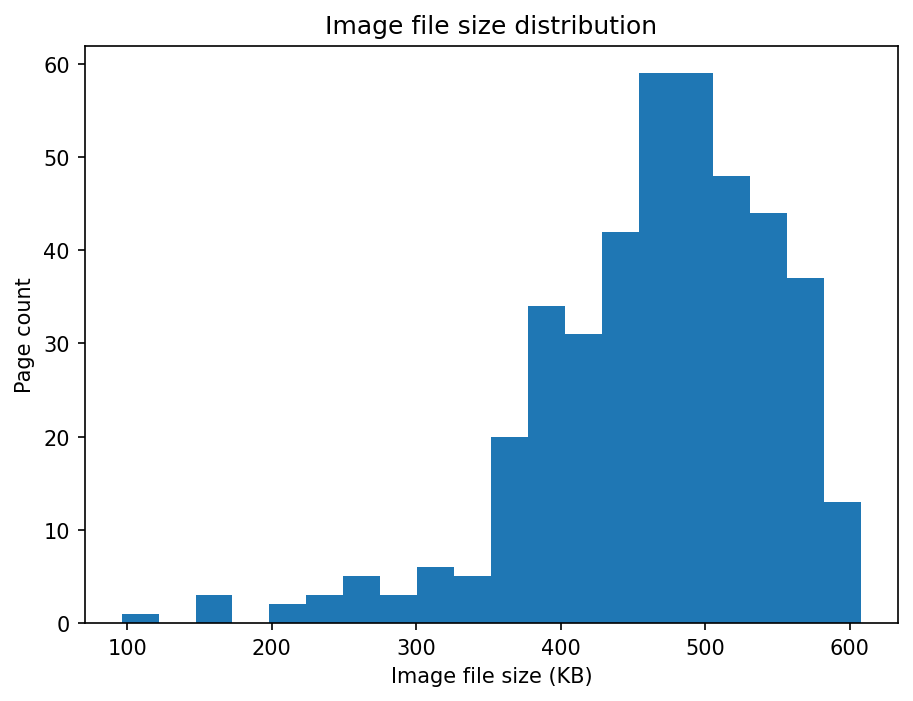
\includegraphics[width=0.85\linewidth,height=\textheight,keepaspectratio]{figures/corpus/file_size_distribution.png}

}

\subcaption{\label{fig-file-size}File size distribution across the
5-book subset}

\end{minipage}%
\newline
\begin{minipage}[t]{\linewidth}

\centering{

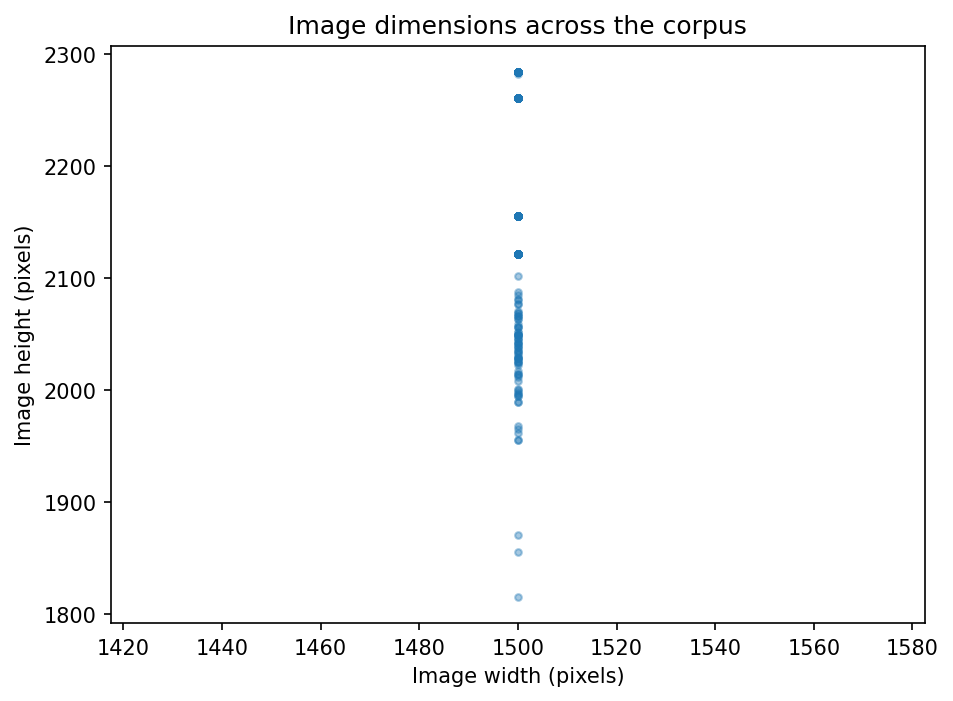
\includegraphics[width=0.85\linewidth,height=\textheight,keepaspectratio]{figures/corpus/image_dimensions_scatter.png}

}

\subcaption{\label{fig-image-dim}Image-dimension scatter showing the
uniform 1500-pixel width}

\end{minipage}%
\newline
\begin{minipage}[t]{\linewidth}

\centering{

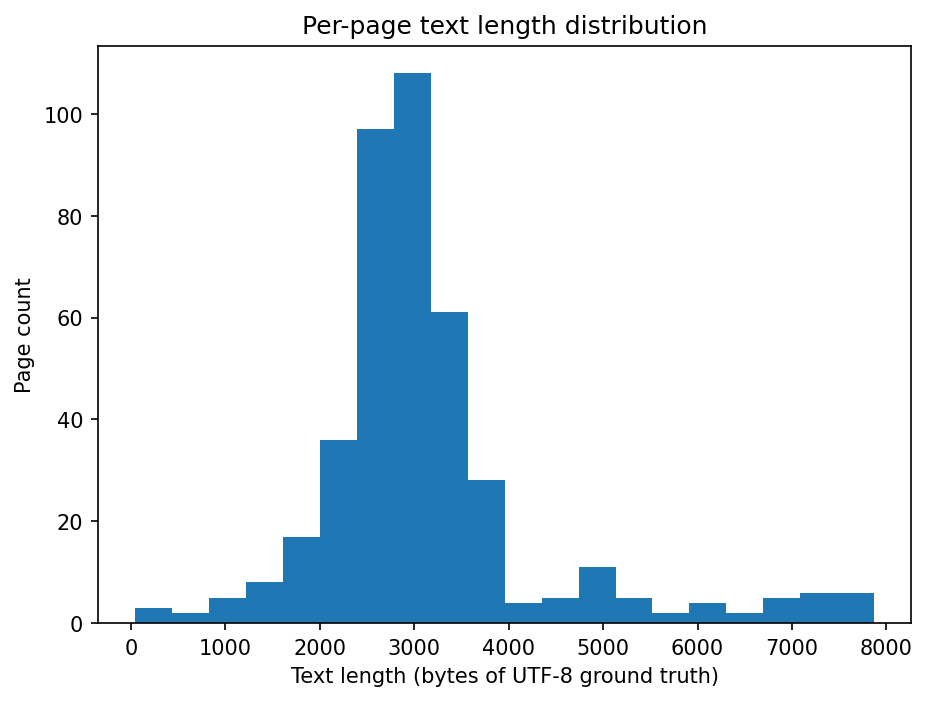
\includegraphics[width=0.85\linewidth,height=\textheight,keepaspectratio]{figures/corpus/text_length_distribution.png}

}

\subcaption{\label{fig-text-len}Page-text-length distribution}

\end{minipage}%

\caption{\label{fig-corpus-distributions}Three distribution plots from
the Phase 1 corpus characterization.}

\end{figure}%

\subsection{Quality taxonomy}\label{quality-taxonomy}

We tagged 97 pages by hand into five quality buckets, then drew the
30-page evaluation subset by stratified random sampling (6 pages per
bucket).

{\def\LTcaptype{none} % do not increment counter
\begin{longtable}[]{@{}
  >{\raggedright\arraybackslash}p{(\linewidth - 4\tabcolsep) * \real{0.2051}}
  >{\raggedright\arraybackslash}p{(\linewidth - 4\tabcolsep) * \real{0.3333}}
  >{\raggedright\arraybackslash}p{(\linewidth - 4\tabcolsep) * \real{0.4615}}@{}}
\toprule\noalign{}
\begin{minipage}[b]{\linewidth}\raggedright
Bucket
\end{minipage} & \begin{minipage}[b]{\linewidth}\raggedright
Description
\end{minipage} & \begin{minipage}[b]{\linewidth}\raggedright
Per-bucket count
\end{minipage} \\
\midrule\noalign{}
\endhead
\bottomrule\noalign{}
\endlastfoot
Clean & Sharp scan, no skew, no fading, simple layout & 6 \\
Skewed & Visible rotation; characters intact & 6 \\
Faded & Reduced contrast; faint character strokes & 6 \\
Complex Layout & Multi-column, ornamental dividers, decorative borders &
6 \\
Damaged & Physical damage, missing content, torn pages & 6 \\
\end{longtable}
}

\begin{figure}[H]

\begin{minipage}[t]{0.33\linewidth}

\centering{

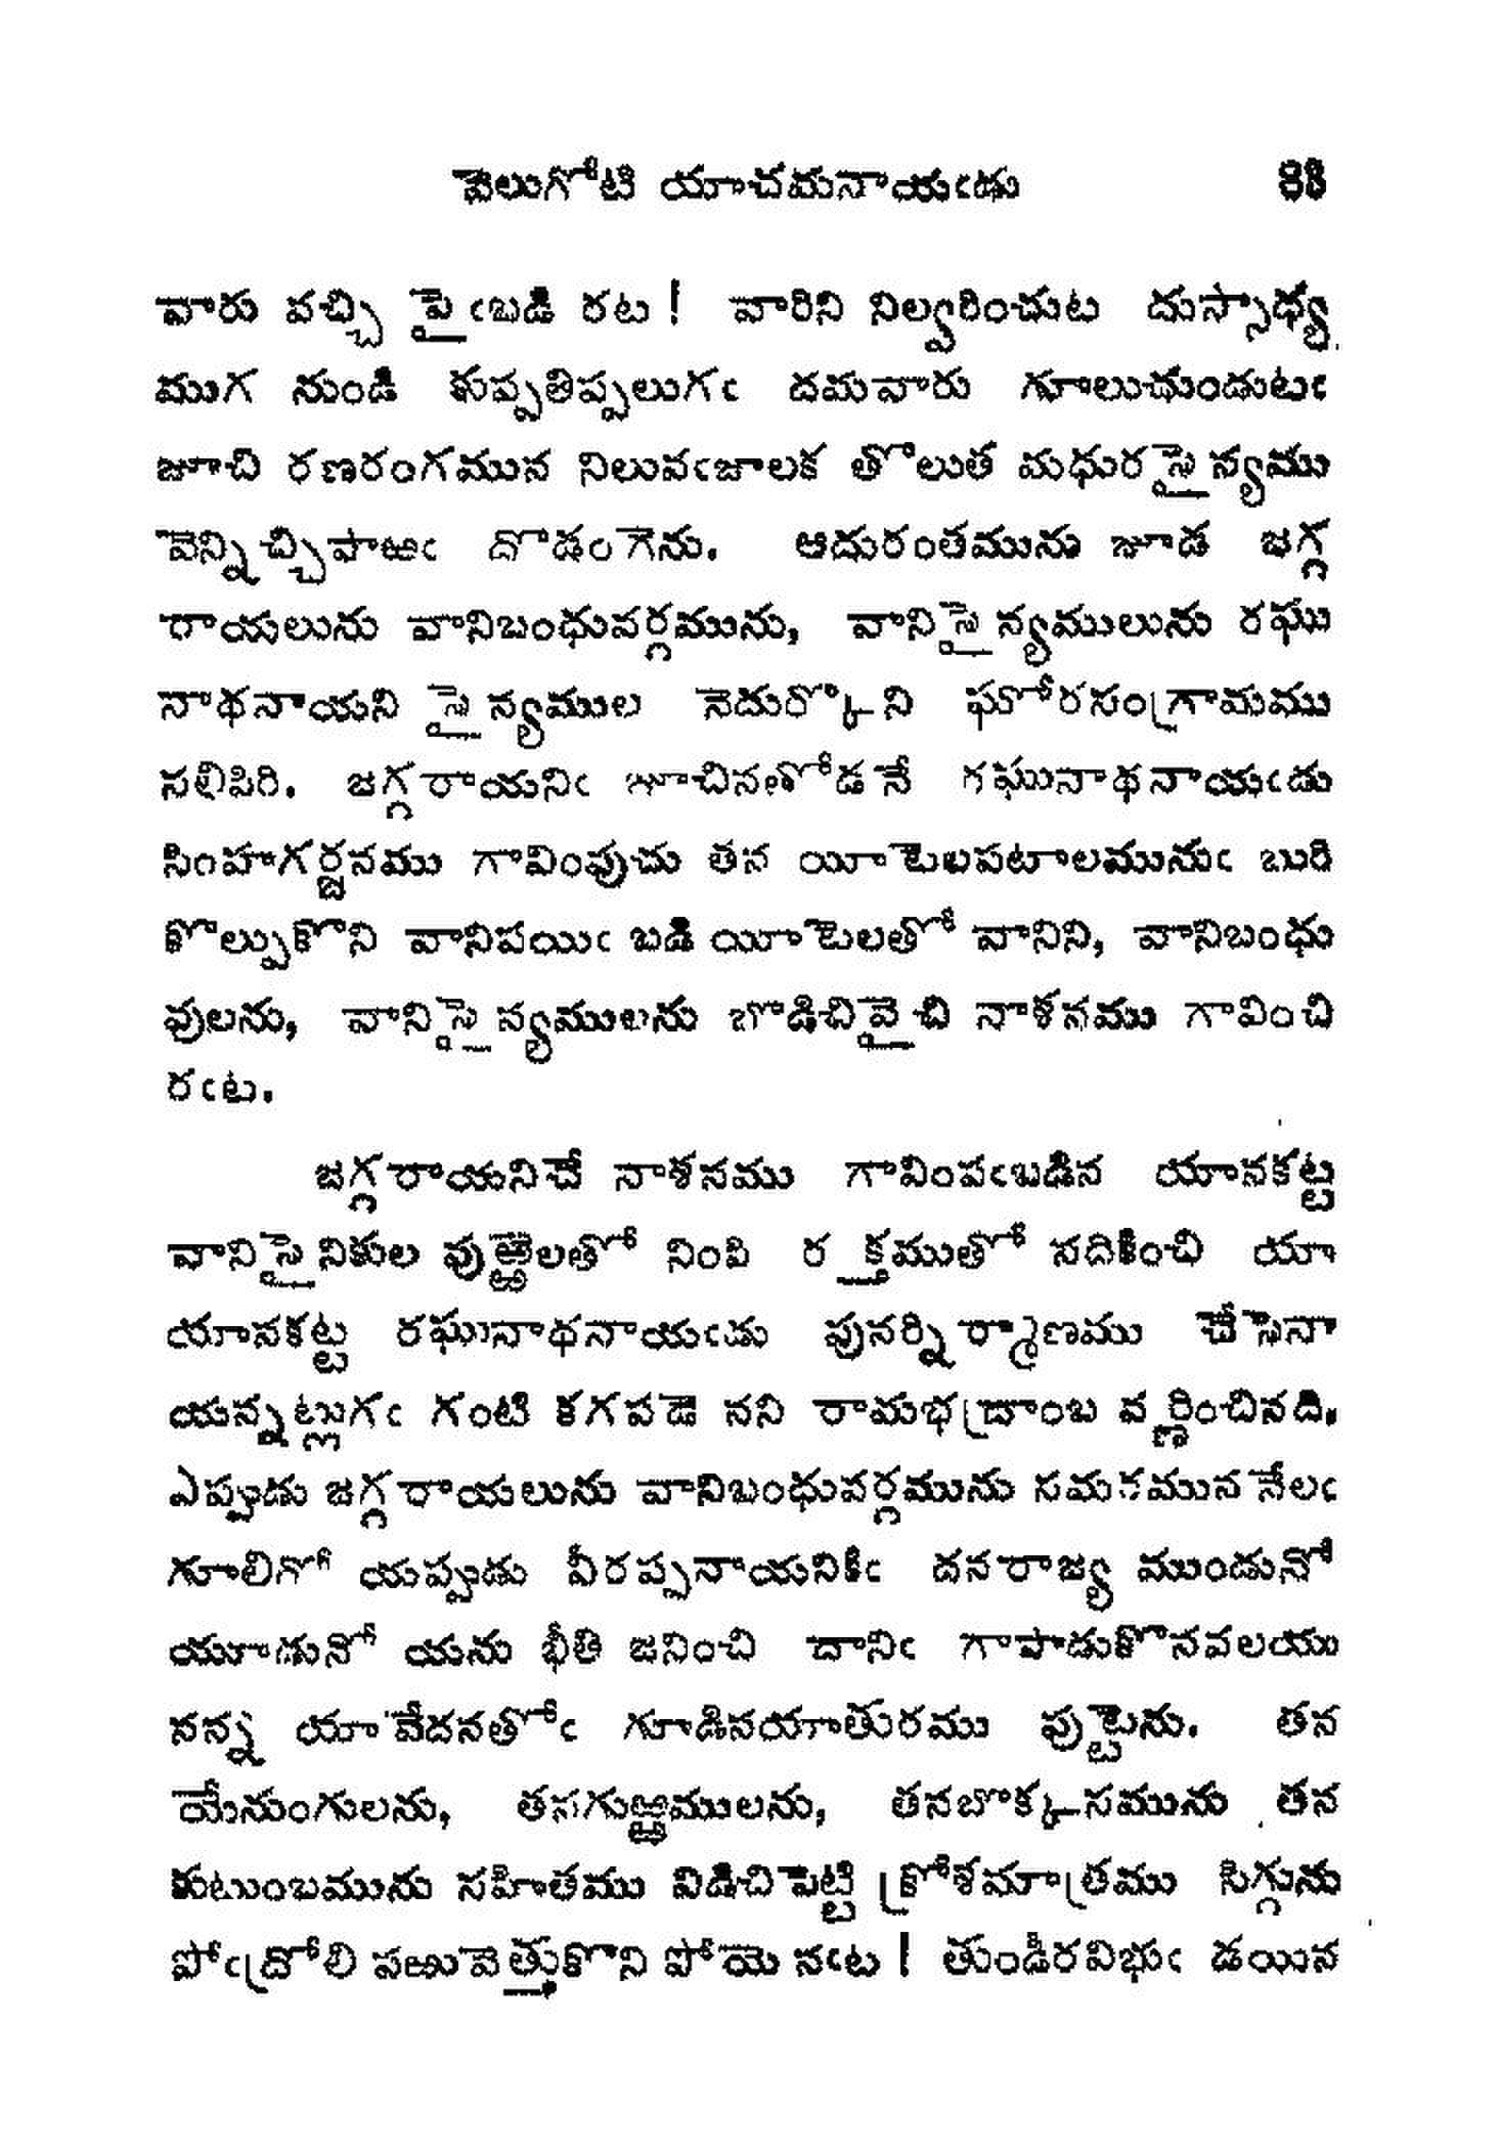
\includegraphics[width=1\linewidth,height=\textheight,keepaspectratio]{figures/corpus/quality_examples/clean.jpg}

}

\subcaption{\label{fig-clean}Clean}

\end{minipage}%
%
\begin{minipage}[t]{0.33\linewidth}

\centering{

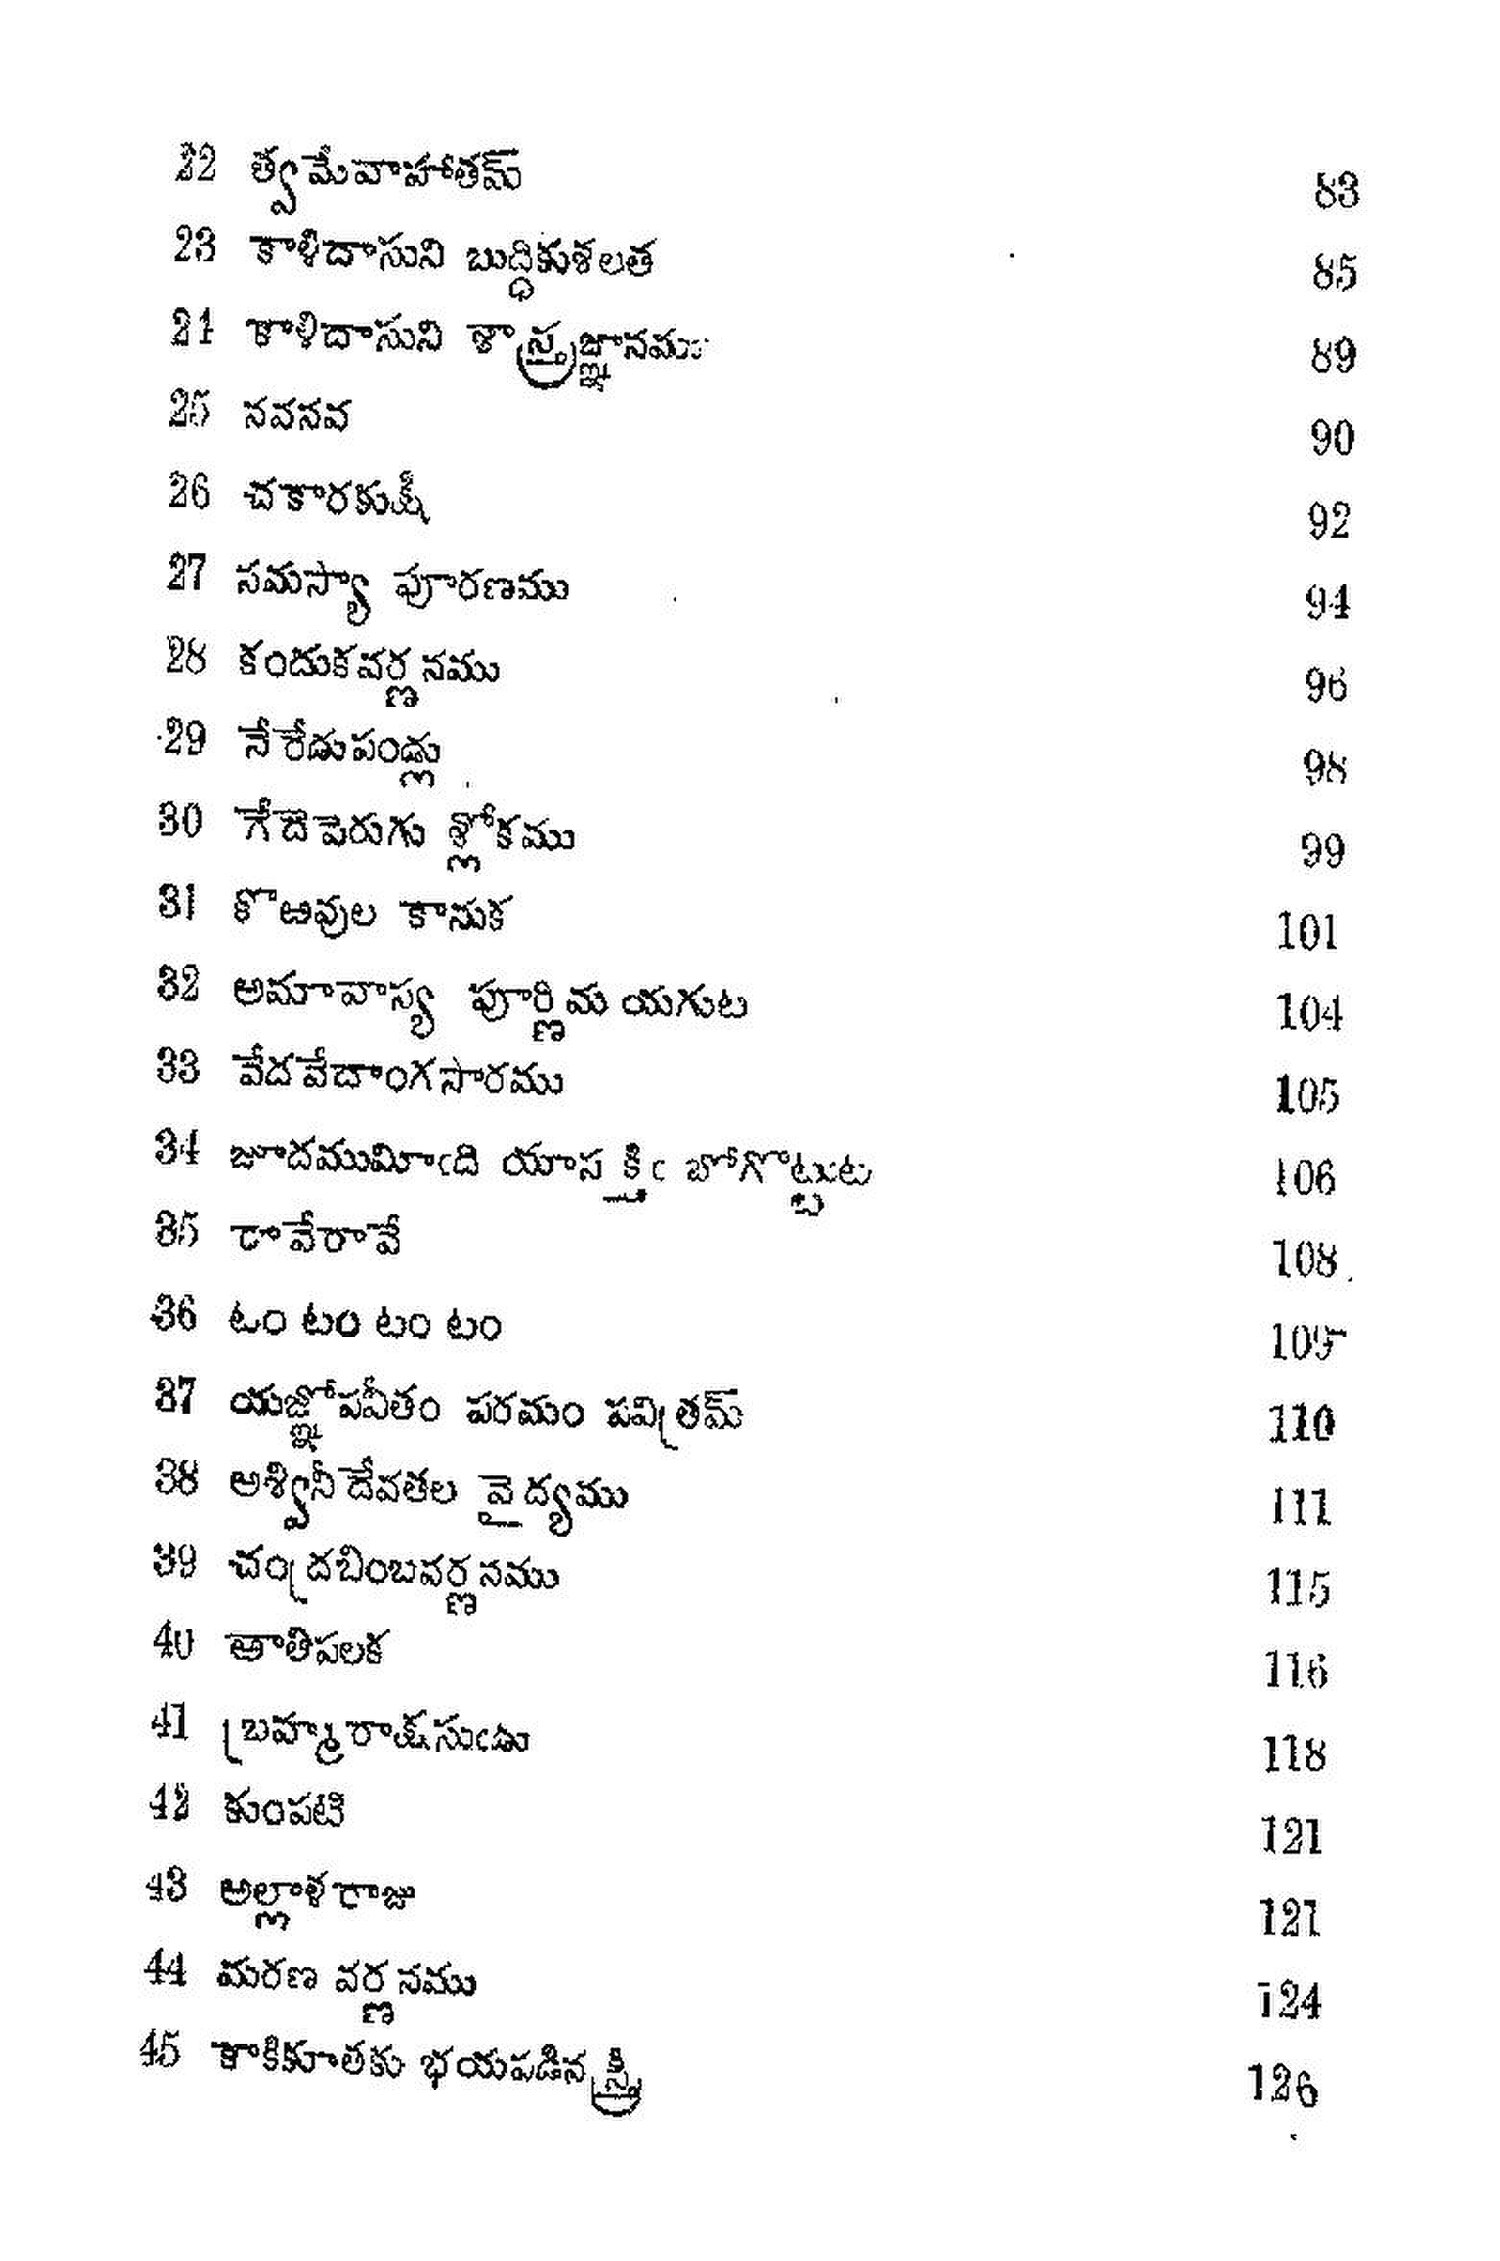
\includegraphics[width=1\linewidth,height=\textheight,keepaspectratio]{figures/corpus/quality_examples/skewed.jpg}

}

\subcaption{\label{fig-skewed}Skewed}

\end{minipage}%
%
\begin{minipage}[t]{0.33\linewidth}

\centering{

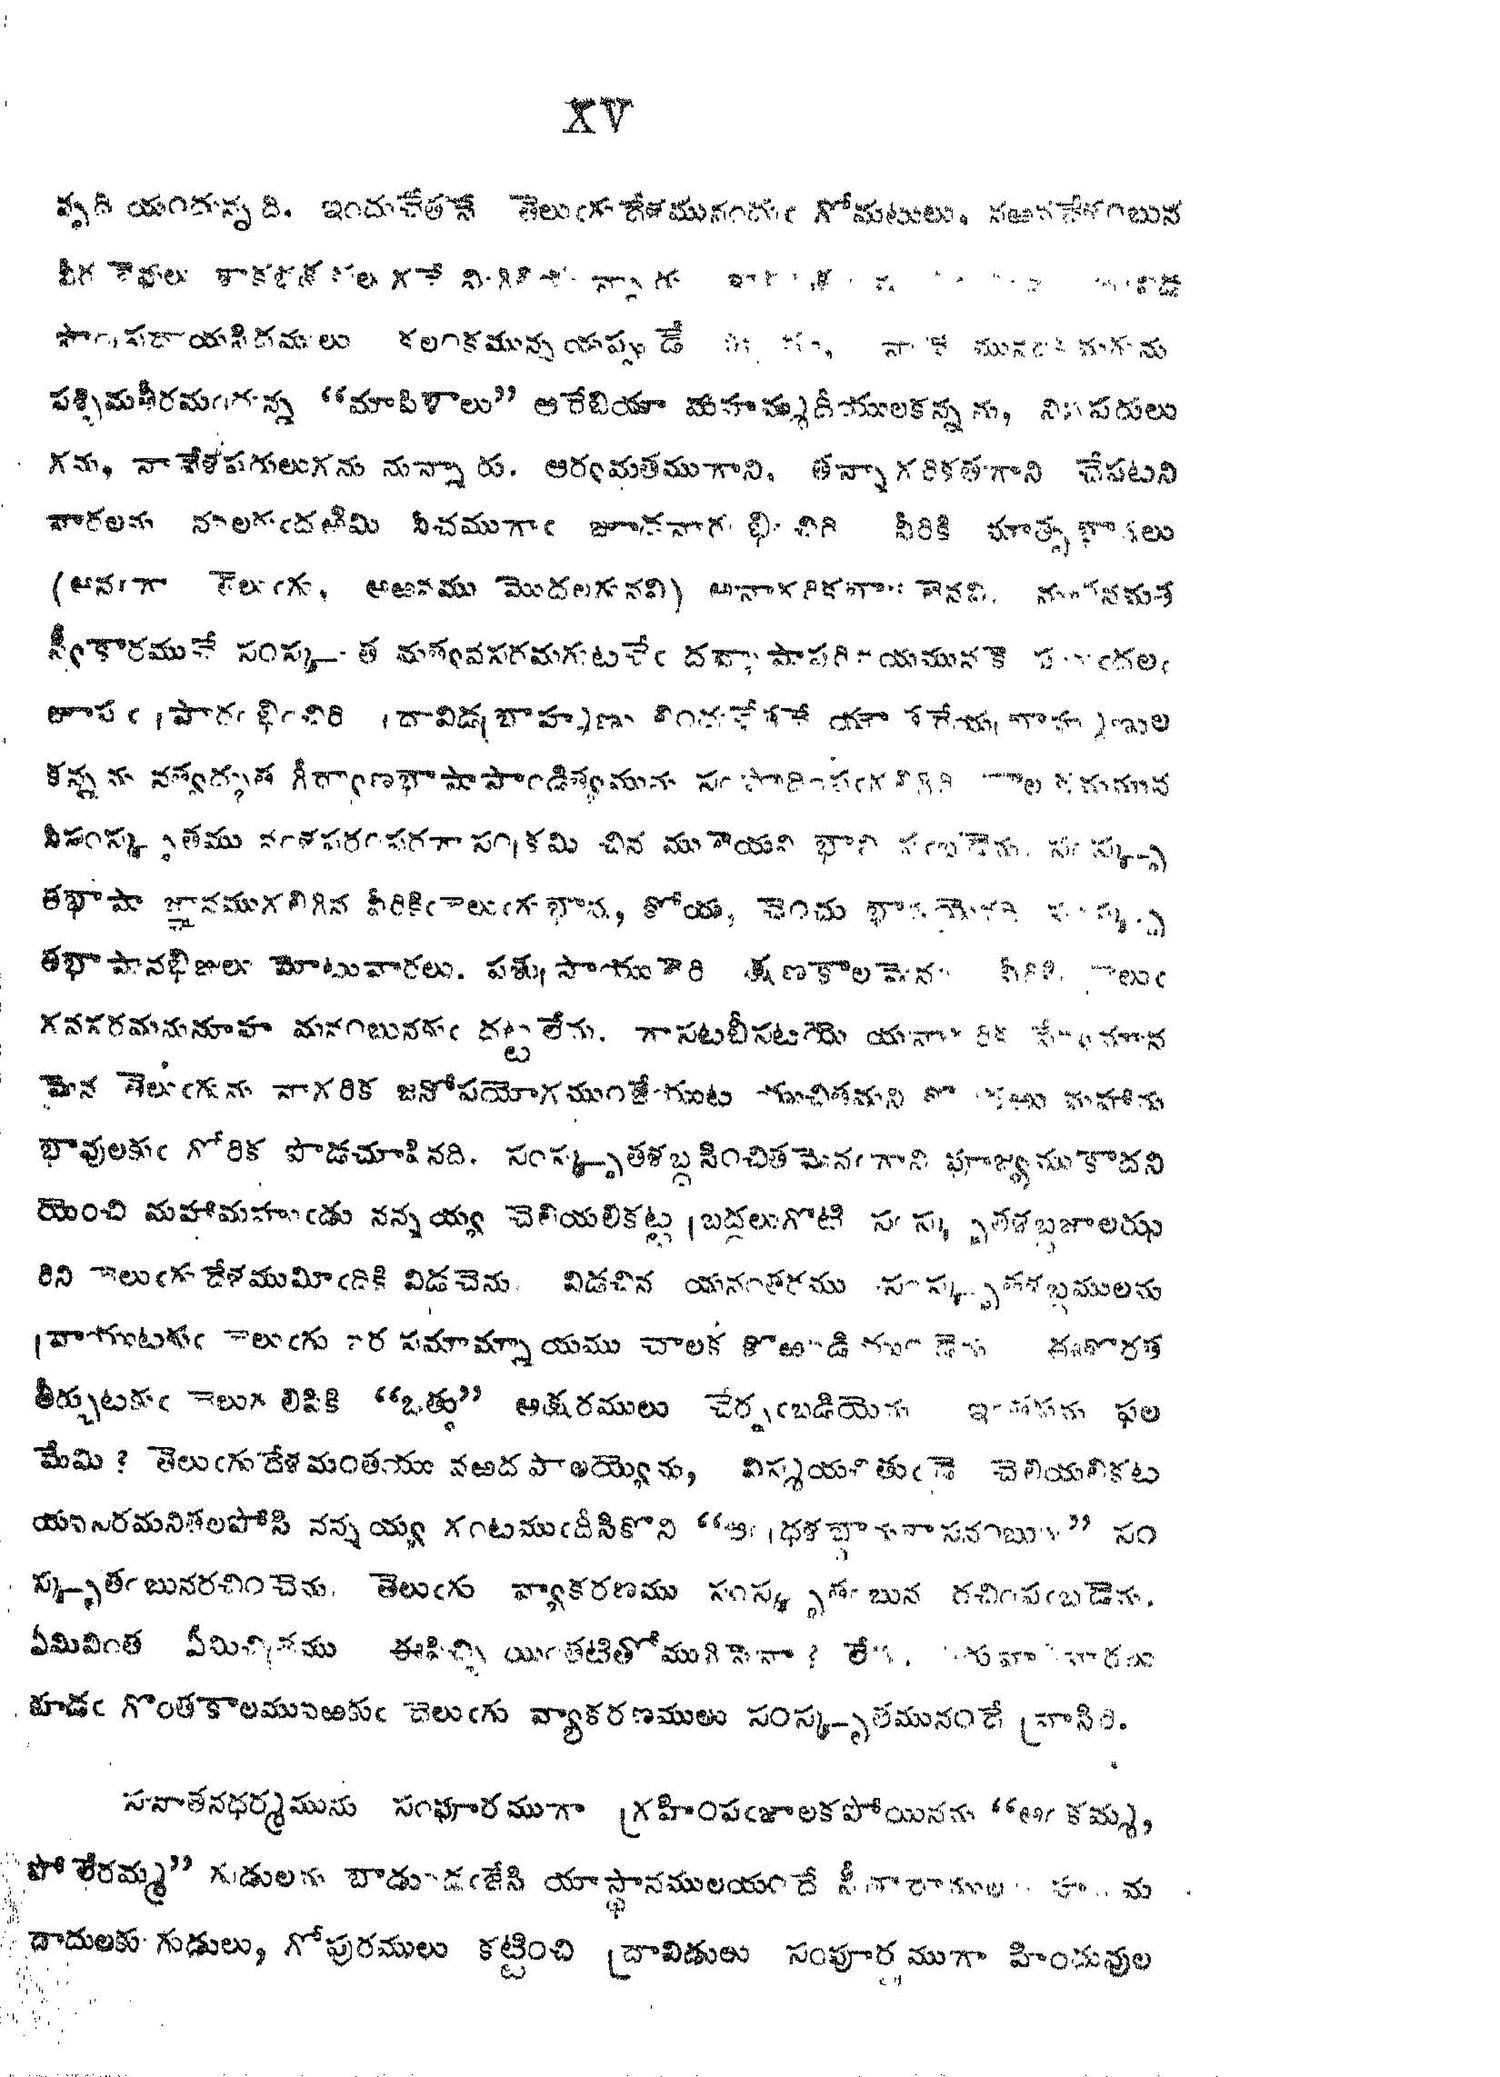
\includegraphics[width=1\linewidth,height=\textheight,keepaspectratio]{figures/corpus/quality_examples/faded.jpg}

}

\subcaption{\label{fig-faded}Faded}

\end{minipage}%
\newline
\begin{minipage}[t]{0.33\linewidth}

\centering{

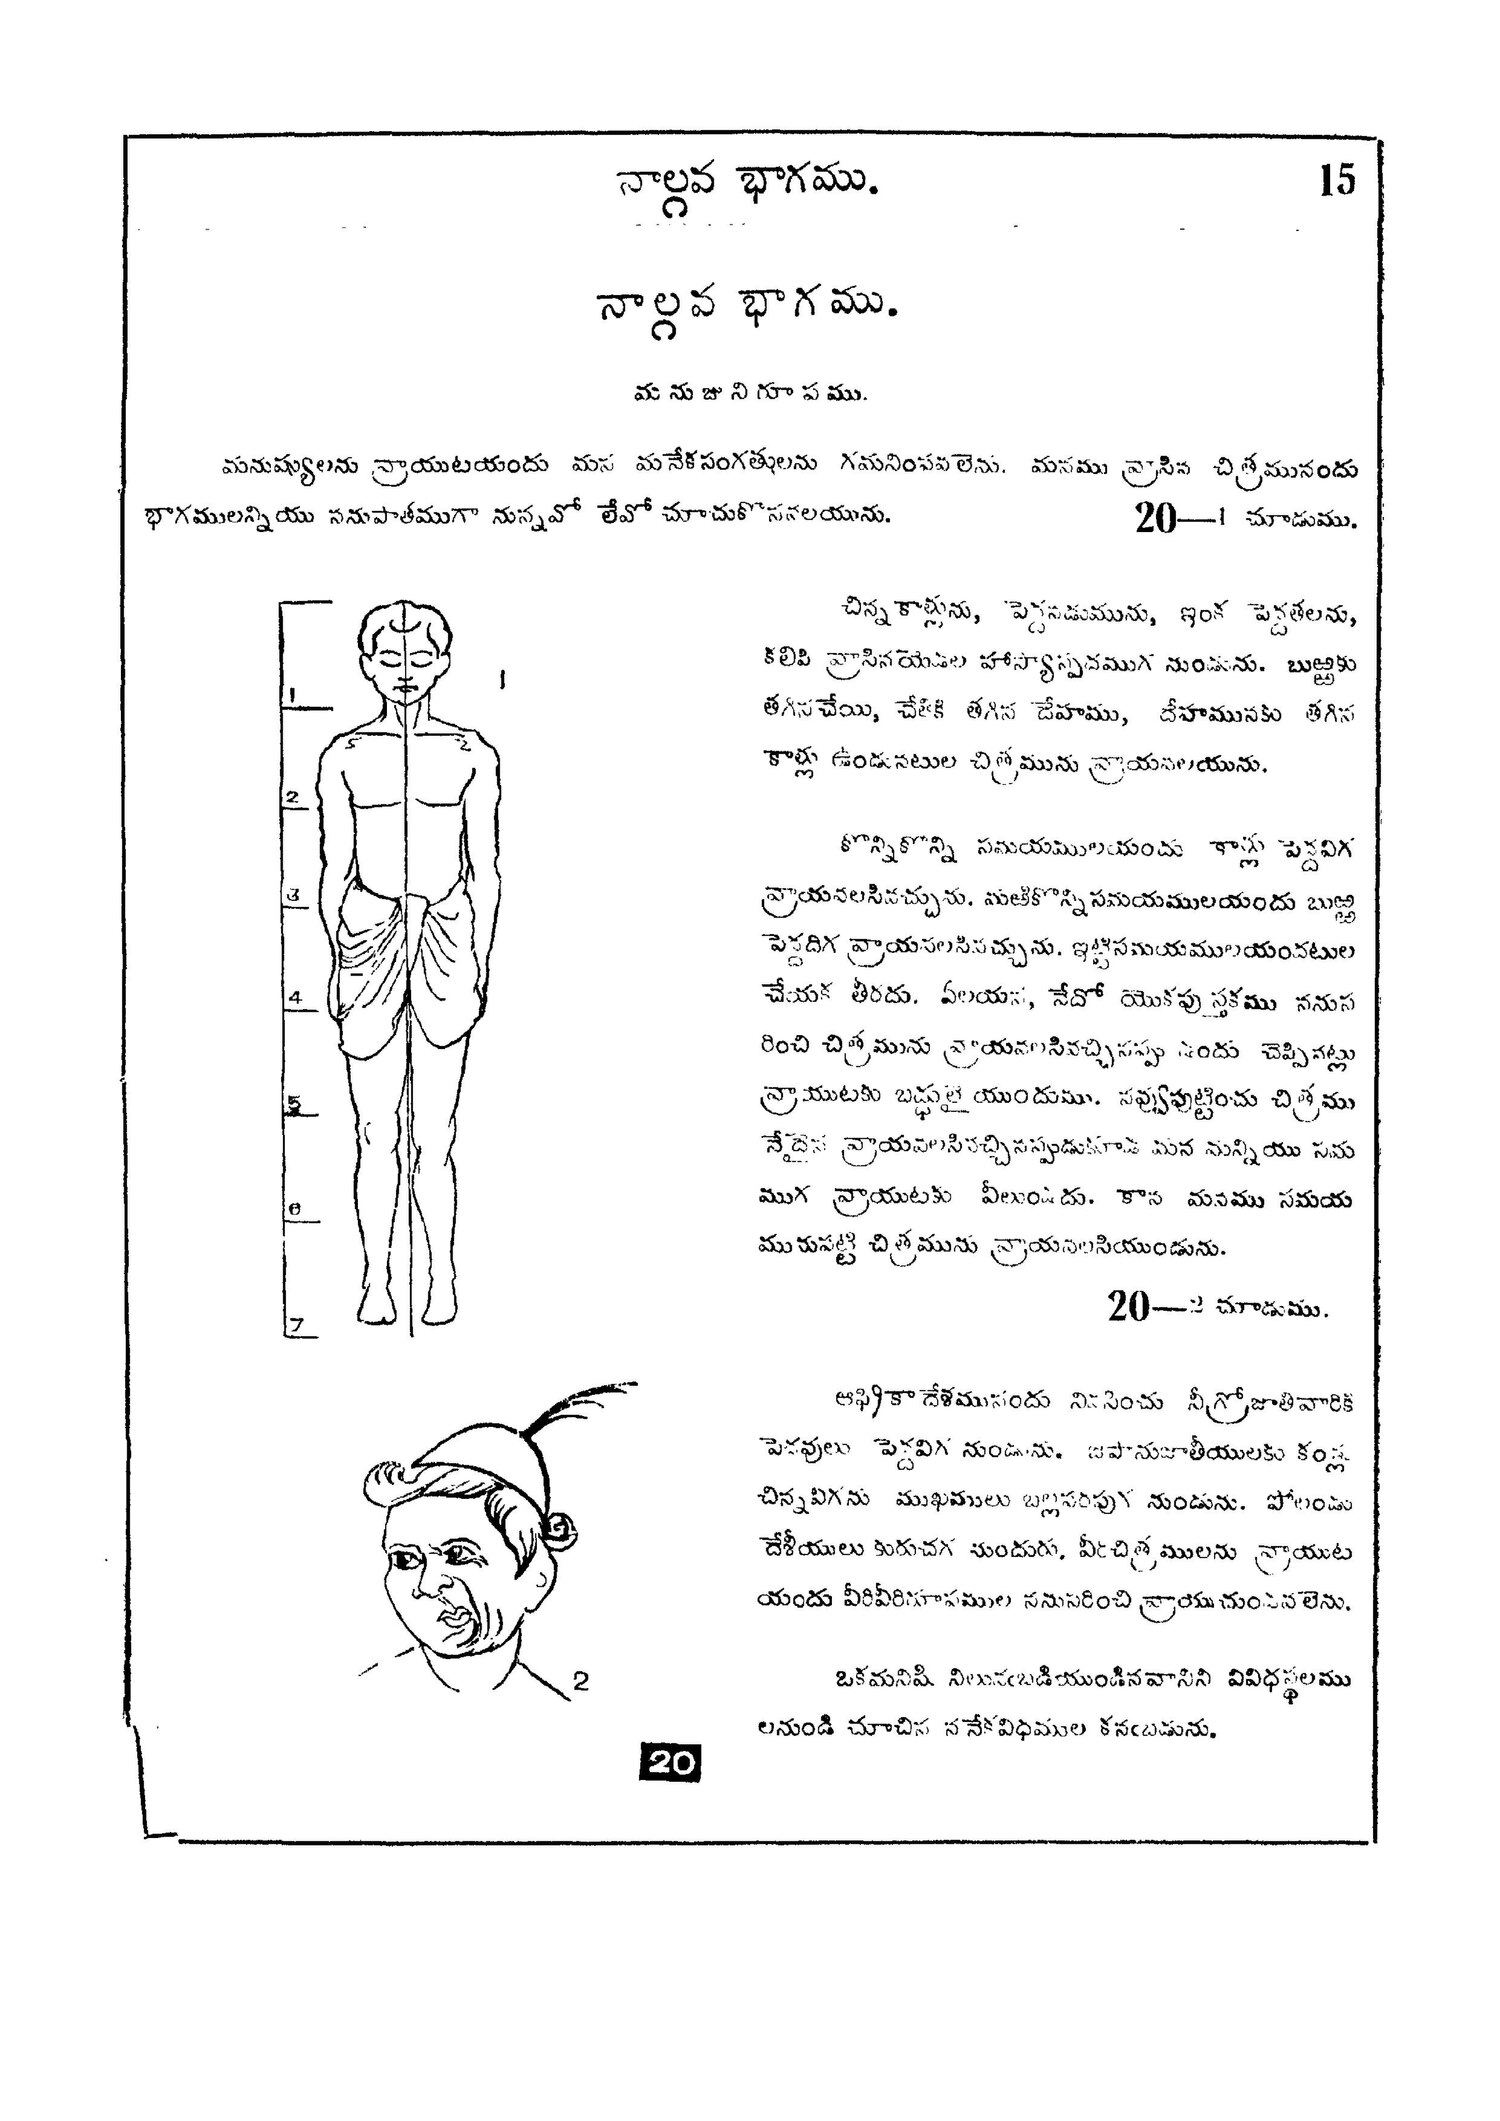
\includegraphics[width=1\linewidth,height=\textheight,keepaspectratio]{figures/corpus/quality_examples/complex_layout.jpg}

}

\subcaption{\label{fig-complex}Complex Layout}

\end{minipage}%
%
\begin{minipage}[t]{0.33\linewidth}

\centering{

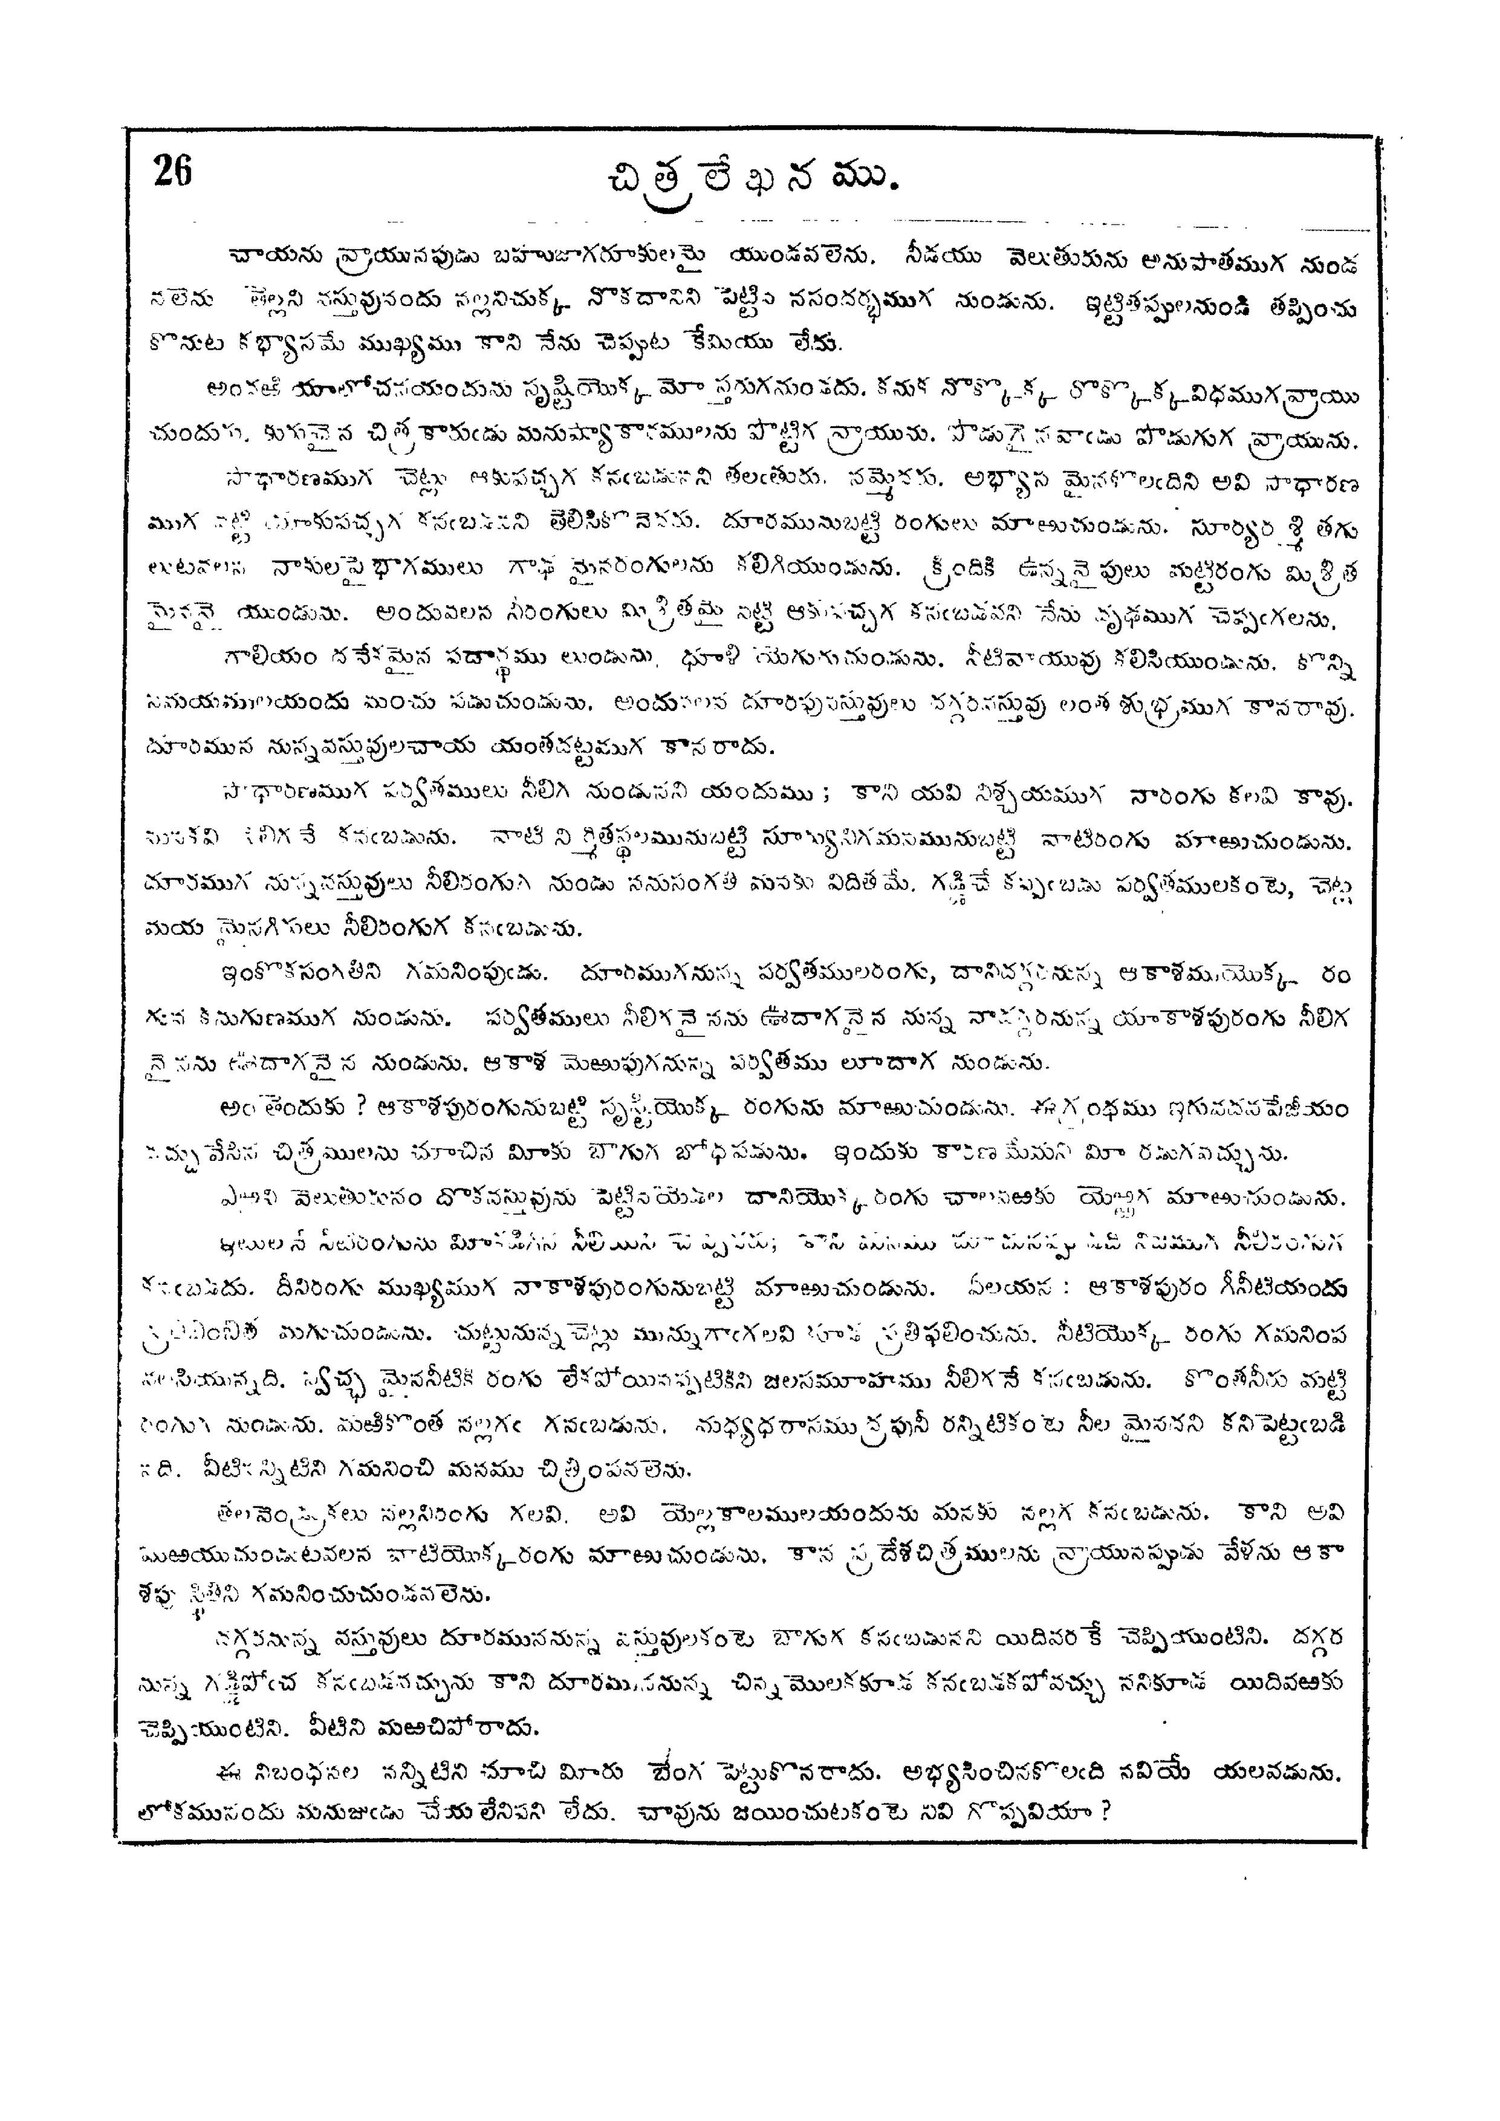
\includegraphics[width=1\linewidth,height=\textheight,keepaspectratio]{figures/corpus/quality_examples/damaged.jpg}

}

\subcaption{\label{fig-damaged}Damaged}

\end{minipage}%

\caption{\label{fig-quality-examples}One example page per quality bucket
from the eval subset.}

\end{figure}%

The taxonomy emerged from browsing the data rather than from an a-priori
spec. Two discoveries during the browse changed our analytical
methodology:

\begin{enumerate}
\def\labelenumi{\arabic{enumi}.}
\tightlist
\item
  \textbf{All images in our 5-book subset are exactly 1500 pixels wide.}
  The ``DPI distribution'' we had planned to report collapsed to a
  single value (\textasciitilde250 DPI based on a typical 6-inch printed
  book width). The corpus-stats JSON records
  \texttt{image\_width\_uniform:\ true}.
\item
  \textbf{Telugu publishing-specific features.} Ornamental section
  dividers (rows of stars/dots), numbered verses in English digits, and
  decorative borders are NOT quality defects but standard typography.
  Disambiguating these from genuine layout complexity required judgment
  we did not anticipate.
\end{enumerate}

These observations are themselves an iteration finding and are discussed
in Section 7.

\subsection{Evaluation subset
construction}\label{evaluation-subset-construction}

\texttt{scripts/select\_eval\_subset.py} draws 6 pages from each quality
bucket using a fixed random seed (42), producing
\texttt{data/external/eval\_subset.csv} and a frozen directory of 30
paired image-and-truth files at \texttt{data/external/eval\_subset/}.
The subset is committed to git so every downstream phase scores against
the same pages.

\begin{center}\rule{0.5\linewidth}{0.5pt}\end{center}

\section{Methodology}\label{methodology}

\subsection{Preprocessing pipeline}\label{preprocessing-pipeline}

\texttt{src/preprocessing/pipeline.py} exposes a composable two-stage
pipeline:

\begin{enumerate}
\def\labelenumi{\arabic{enumi}.}
\tightlist
\item
  \textbf{Deskew} --- \texttt{src.preprocessing.deskew} estimates the
  dominant rotation angle via projection-profile analysis and
  counter-rotates to within ±0.5°. The rotation interpolation is
  bilinear; the canvas is white-padded so corners remain consistent.
\item
  \textbf{Binarize} --- OpenCV (Bradski 2000)
  \texttt{cv2.adaptiveThreshold} with \texttt{block\_size=11,\ c=2}
  (mean Gaussian neighborhood, subtractive constant), Gaussian local
  adaptive thresholding. Output is single-channel uint8 with two values:
  0 (text) and 255 (background).
\item
  \textbf{Denoise} (added during the Phase 5 ablation; see Section 6.3)
  --- OpenCV \texttt{cv2.fastNlMeansDenoising} with \texttt{h=7},
  \texttt{templateWindowSize=7}, \texttt{searchWindowSize=21}.
  Edge-preserving non-local means filter, tuned to preserve thin Telugu
  strokes.
\item
  \textbf{Contrast} (added during the Phase 5 ablation; see Section 6.3)
  --- Contrast Limited Adaptive Histogram Equalization (Zuiderveld 1994)
  via OpenCV \texttt{cv2.createCLAHE} with \texttt{clipLimit=2.0},
  \texttt{tileGridSize=(8,8)}. For BGR input we convert to LAB color
  space and CLAHE the L channel only to avoid per-channel color shift.
\end{enumerate}

\begin{figure}[H]

\begin{minipage}[t]{0.50\linewidth}

\raisebox{-\height}{

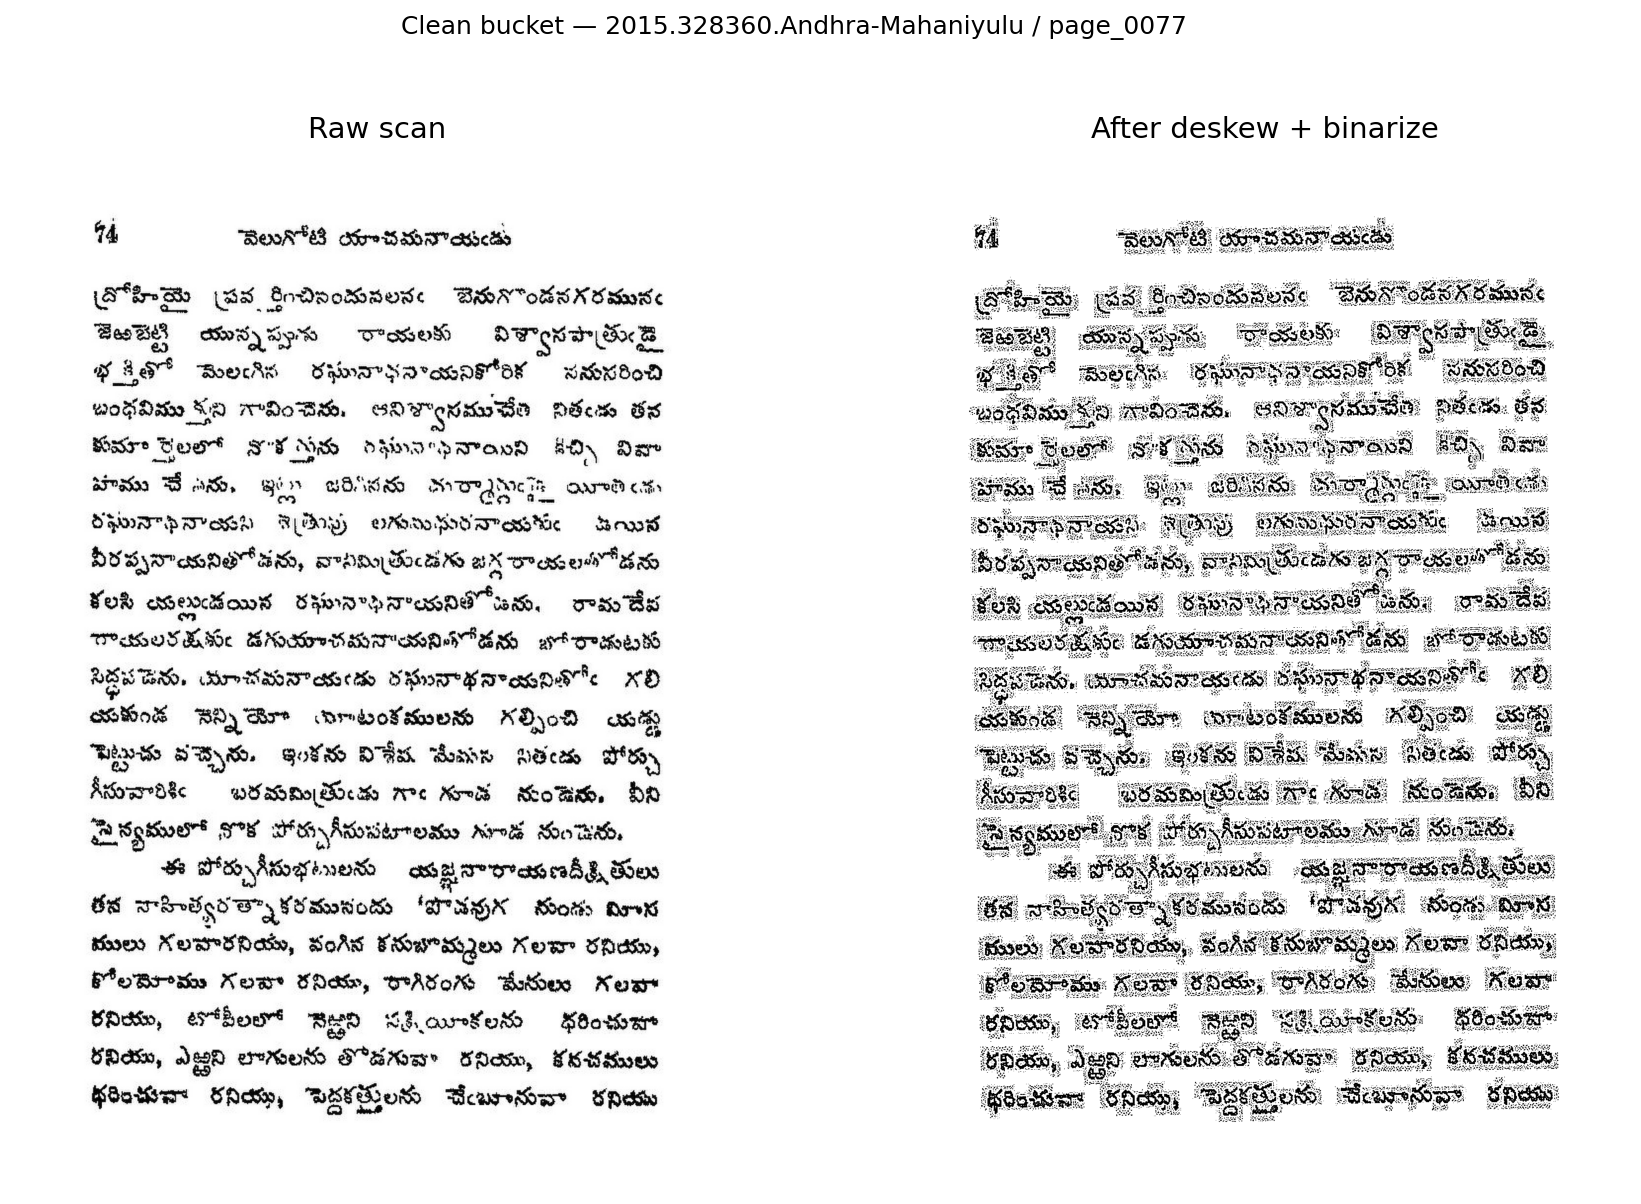
\includegraphics[width=1\linewidth,height=\textheight,keepaspectratio,alt={Clean --- before/after}]{figures/preprocessing/before_after_clean.png}

}

\subcaption{\label{}Clean --- before/after}
\end{minipage}%
%
\begin{minipage}[t]{0.50\linewidth}

\raisebox{-\height}{

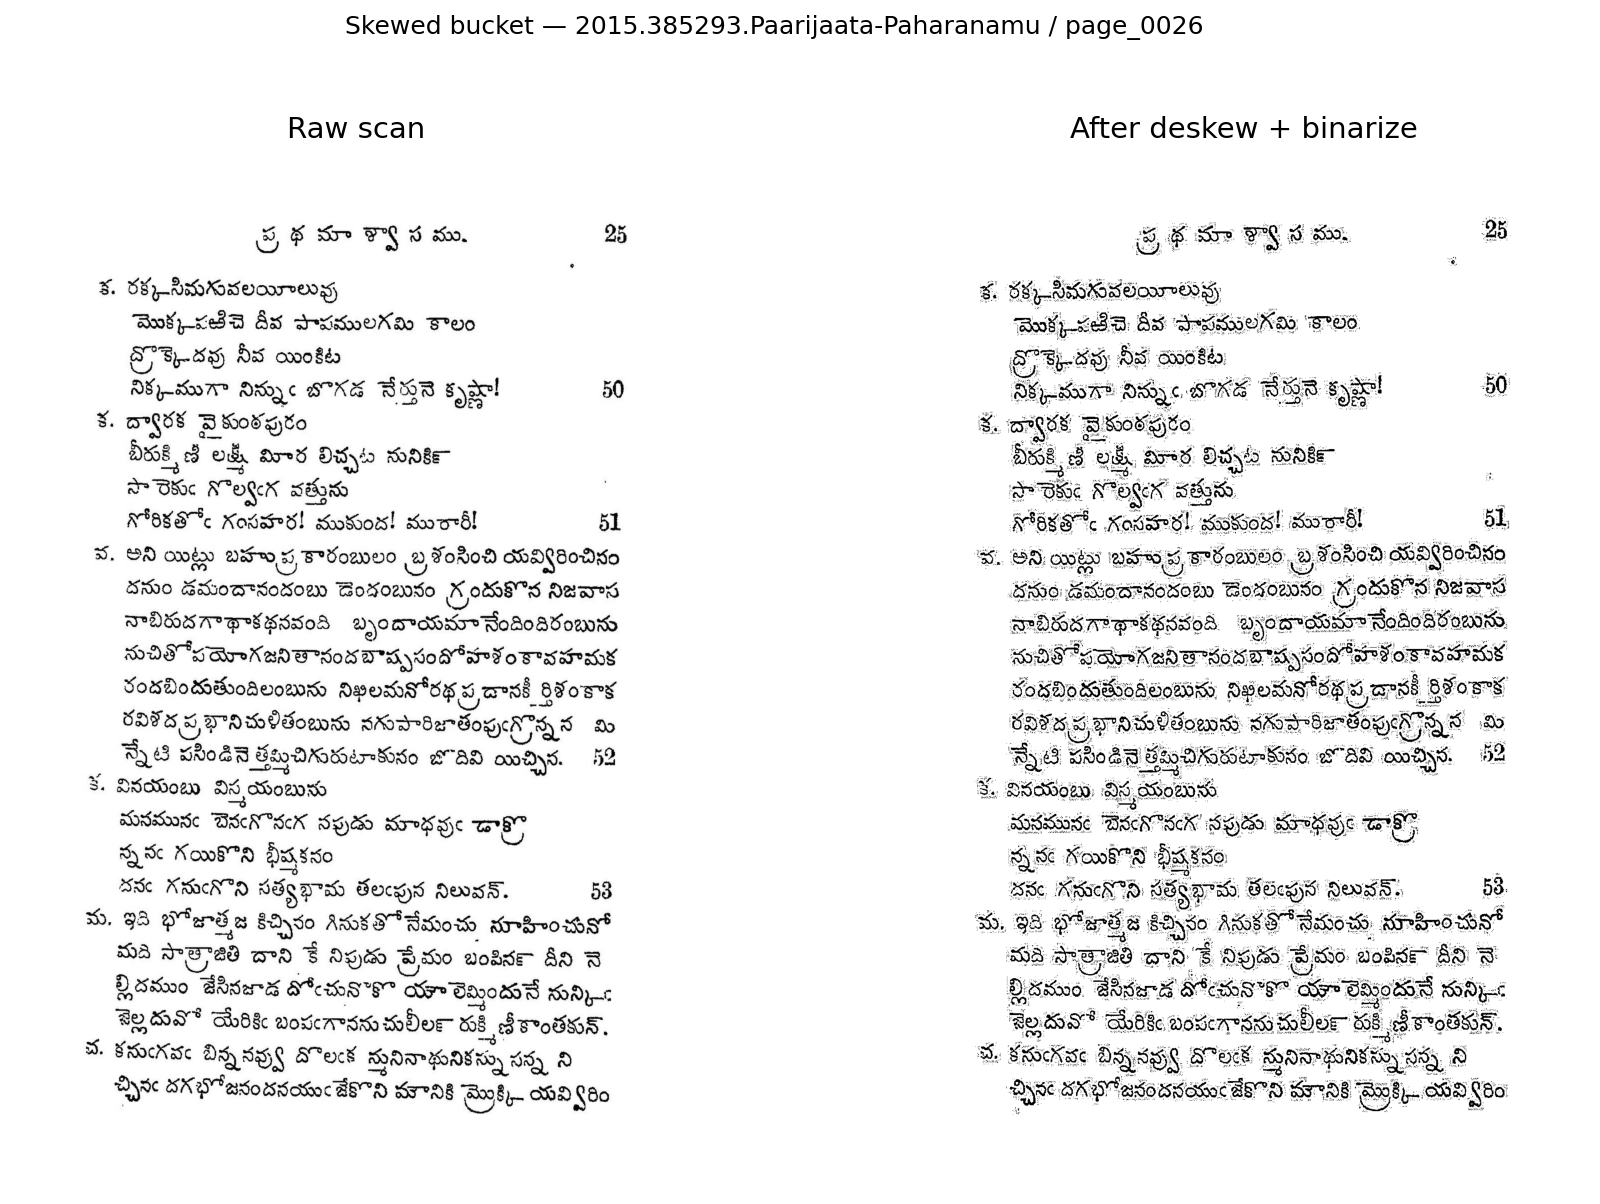
\includegraphics[width=1\linewidth,height=\textheight,keepaspectratio,alt={Skewed --- before/after}]{figures/preprocessing/before_after_skewed.png}

}

\subcaption{\label{}Skewed --- before/after}
\end{minipage}%
\newline
\begin{minipage}[t]{0.50\linewidth}

\raisebox{-\height}{

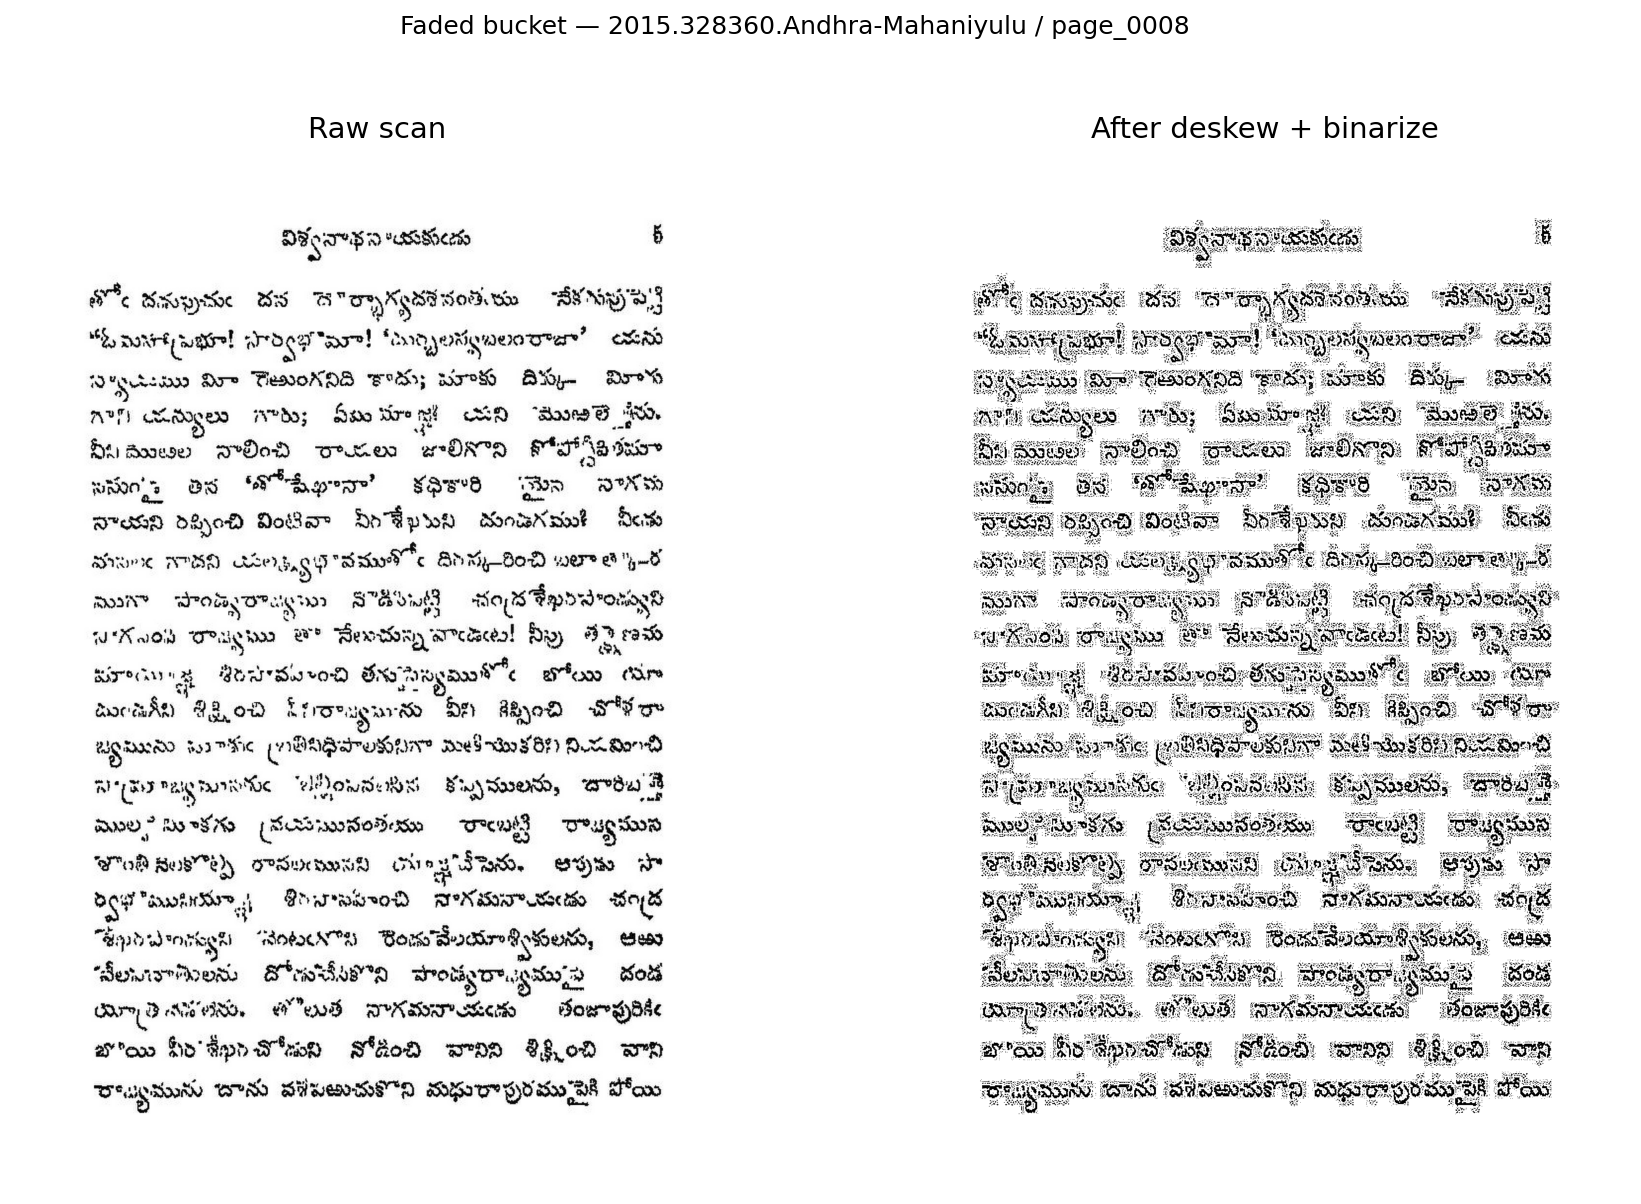
\includegraphics[width=1\linewidth,height=\textheight,keepaspectratio,alt={Faded --- before/after}]{figures/preprocessing/before_after_faded.png}

}

\subcaption{\label{}Faded --- before/after}
\end{minipage}%
%
\begin{minipage}[t]{0.50\linewidth}

\raisebox{-\height}{

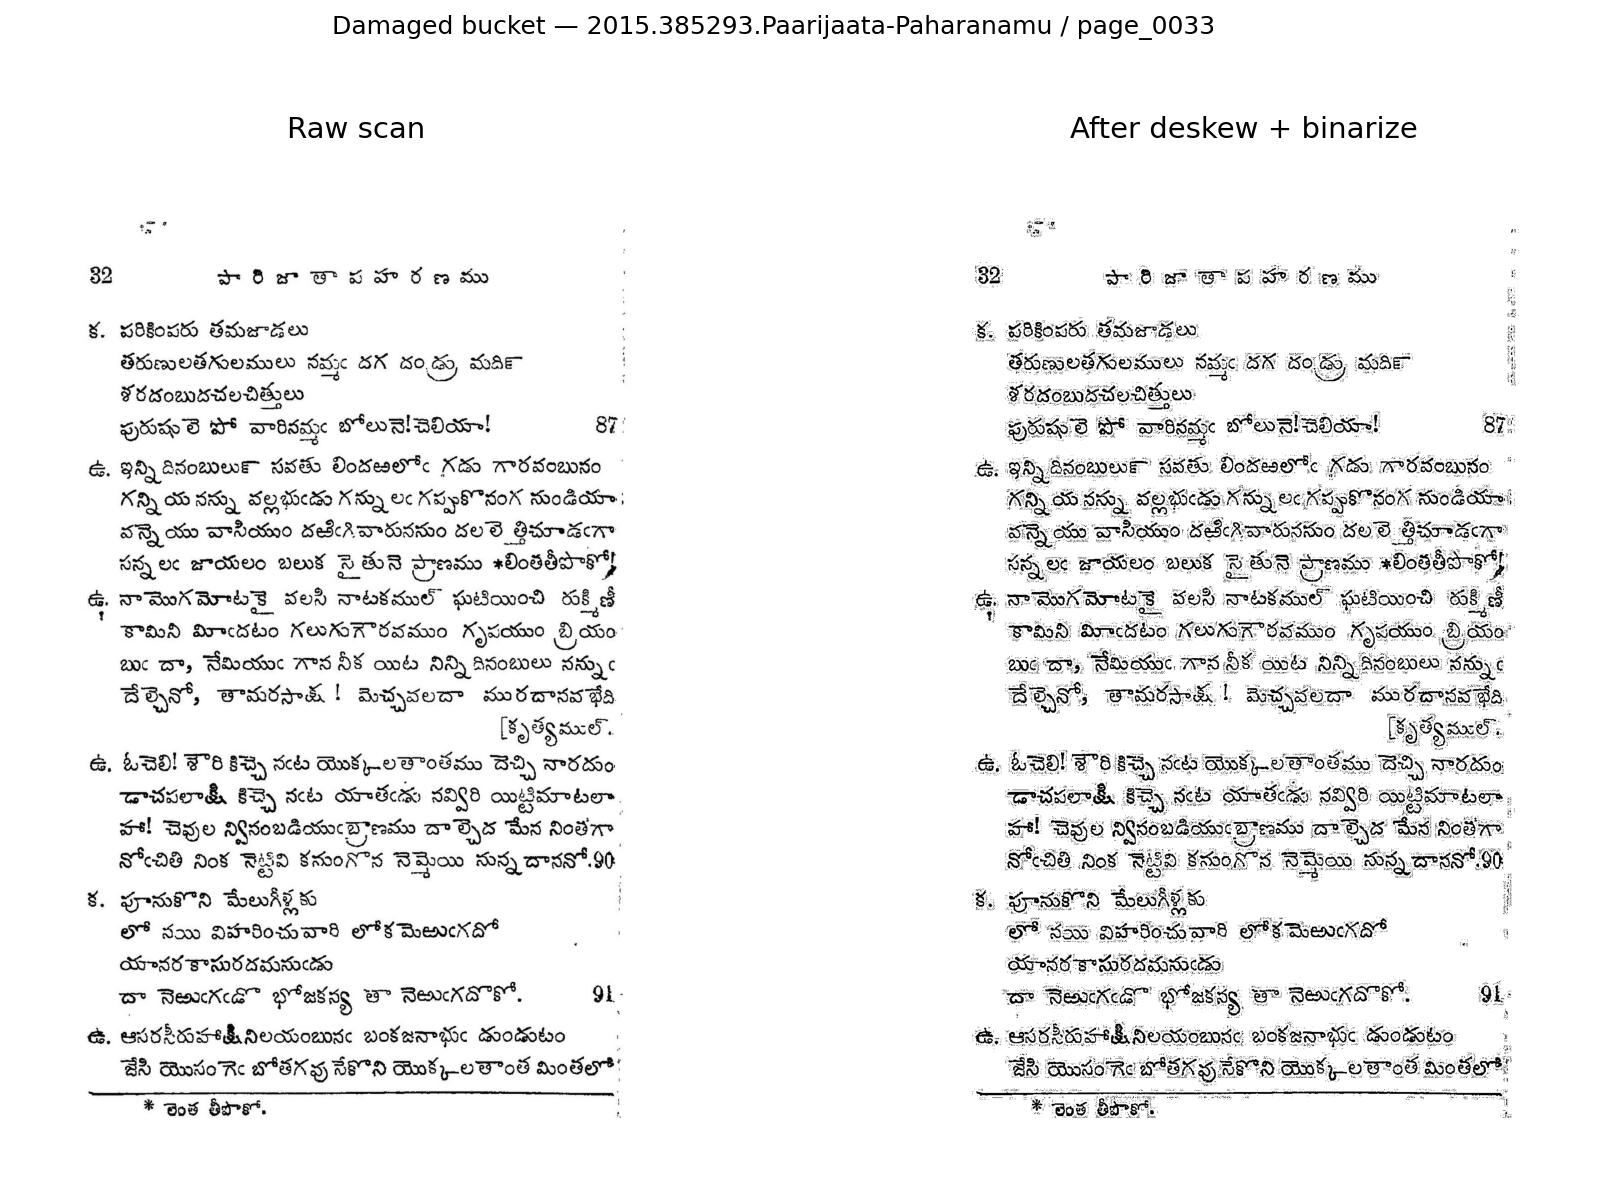
\includegraphics[width=1\linewidth,height=\textheight,keepaspectratio,alt={Damaged --- before/after}]{figures/preprocessing/before_after_damaged.png}

}

\subcaption{\label{}Damaged --- before/after}
\end{minipage}%

\caption{\label{fig-preprocessing}Before/after the two-stage
preprocessing pipeline (deskew + binarize), one per quality bucket where
the effect is visible.}

\end{figure}%

Stages 1 and 2 (deskew + binarize) shipped in the Phase 2 deliverable.
Stages 3 and 4 (denoise + contrast) were originally deferred for time,
then implemented late in Phase 5 to support the per-stage ablation (see
Section 6.3). All four stages are now part of
\texttt{src/preprocessing/}, with per-stage enable/disable via
\texttt{Pipeline.run(...,\ enable=\{...\})} so any subset can be applied
to test specific hypotheses.

\subsection{OCR adapters}\label{ocr-adapters}

\texttt{src/ocr/} defines an \texttt{OCRAdapter} Protocol that every
backend satisfies:

\begin{Shaded}
\begin{Highlighting}[]
\KeywordTok{class}\NormalTok{ OCRAdapter(Protocol):}
\NormalTok{    model\_name: }\BuiltInTok{str}
    \KeywordTok{def}\NormalTok{ ocr(}\VariableTok{self}\NormalTok{, image\_path: Path) }\OperatorTok{{-}\textgreater{}}\NormalTok{ OCRResult: ...}
\end{Highlighting}
\end{Shaded}

Four implementations:

\begin{itemize}
\tightlist
\item
  \texttt{src.ocr.tesseract.TesseractAdapter} --- wraps the pinned
  \texttt{ml-class-project/tesseract} Docker image (Tesseract 5, Telugu
  language pack, PSM 6).
\item
  \texttt{src.ocr.gemini.GeminiAdapter} --- Google Gemini 2.5 Flash via
  the \texttt{google-generativeai} SDK (Google 2026b).
\item
  \texttt{src.ocr.claude.ClaudeAdapter} --- Anthropic Claude Sonnet 4.6
  by default, with constructor override for Opus 4.8, via the
  \texttt{anthropic} Python SDK (Anthropic 2026a).
\end{itemize}

Every adapter NFC-normalizes its output text, returns latency in
milliseconds, and surfaces empty/refusal outputs as
\texttt{OCRResult(text="",\ ...)} rather than raising --- so a batch run
never aborts on a single bad page.

The batch runner \texttt{scripts/run\_ocr.py} walks an input directory
tree and dispatches each page through the chosen adapter, writing one
\texttt{.txt} per page mirroring the input layout, plus a
\texttt{manifest.jsonl} recording per-page latency and any error. The
runner is idempotent: a page whose output already exists is skipped
unless \texttt{-\/-overwrite} is given. This let us re-run the eval
matrix and incrementally extend the submission sample from 415 to 524+
pages (after we added a 6th book) without re-paying API costs for pages
already done.

\subsection{Vision-LLM prompt}\label{vision-llm-prompt}

Both Gemini and Claude were prompted with identical text adapted from
the project spec's example prompt. Specifically, we modified the spec's
example to (a) remove the \texttt{{[}?{]}} ambiguity-marker instruction,
which would have introduced \texttt{{[}?{]}} tokens into the OCR output
that downstream CER scoring would penalize, and (b) make NFC Unicode
normalization an explicit requirement (the spec implied it). Both
adapters use the same final prompt, which we lifted verbatim into both
adapter source files so a prompt-variant study can A/B them without
divergence:

\begin{Shaded}
\begin{Highlighting}[]
\NormalTok{You are a Telugu OCR system. Extract all Telugu text from the}
\NormalTok{provided image and return ONLY the Unicode text content. Rules:}
\NormalTok{{-} Output Telugu characters as Unicode (UTF{-}8 NFC).}
\NormalTok{{-} Do NOT translate to English. Do NOT transliterate.}
\NormalTok{{-} Do NOT add any commentary, headers, footers, or markdown.}
\NormalTok{{-} Preserve paragraph breaks with newlines.}
\NormalTok{{-} If a portion of the page is illegible, output what you can}
\NormalTok{  read and skip the rest silently.}
\NormalTok{{-} If the page is empty or contains no text, return an empty}
\NormalTok{  string.}
\end{Highlighting}
\end{Shaded}

We did not run a prompt-variant study; Section 9 (Limitations) discusses
why this remains future work.

\subsection{Evaluation metrics}\label{evaluation-metrics}

\textbf{Classical metrics.} \texttt{src/validation/classical.py} wraps
\texttt{jiwer} with NFC normalization applied to both inputs before
scoring. Two pure functions:

\begin{itemize}
\tightlist
\item
  \texttt{compute\_cer(reference,\ hypothesis)\ -\textgreater{}\ float}
  --- character error rate.
\item
  \texttt{compute\_wer(reference,\ hypothesis)\ -\textgreater{}\ float}
  --- word error rate (whitespace tokenization).
\end{itemize}

Edge cases: empty reference raises \texttt{ValueError} (CER
mathematically undefined); empty hypothesis returns \texttt{1.0} (every
reference character is a deletion).

\textbf{LLM-based validation methods.}

\begin{itemize}
\tightlist
\item
  \textbf{Method A --- fluency scoring}
  (\texttt{src/validation/llm\_fluency.py}). A vision LLM (we used
  Claude Sonnet 4.6 due to Gemini's free-tier rate-limit saturation; see
  Section 6) is asked to rate an OCR output's fluency as Telugu prose on
  a 1--5 integer scale, with a one-sentence reason and up to 3 error
  examples. Output is parsed as strict JSON; deviations raise
  \texttt{FluencyJudgeError} rather than silently defaulting to a median
  rating.
\item
  \textbf{Method B --- cross-model agreement}
  (\texttt{src/validation/agreement.py}). Stdlib-only
  \texttt{difflib.SequenceMatcher.ratio()} on the two NFC-normalized
  texts. Returns a similarity score in \texttt{{[}0.0,\ 1.0{]}}.
  Pairwise and mean-pairwise variants supported.
\end{itemize}

Phase 4 calibrates both methods against the ground-truth CER on the eval
subset; Section 6.5 reports the correlations.

\begin{center}\rule{0.5\linewidth}{0.5pt}\end{center}

\section{Results}\label{results}

\subsection{Per-cell CER and WER}\label{per-cell-cer-and-wer}

The full eval matrix is 4 models × up to 5 preprocessing variants × 30
stratified pages = 510 rows. Claude Opus has 2 variants (raw +
deskew+binarize) for cost reasons; the other 3 models have all 5
variants. Aggregate statistics per cell:

{\def\LTcaptype{none} % do not increment counter
\begin{longtable}[]{@{}
  >{\raggedright\arraybackslash}p{(\linewidth - 12\tabcolsep) * \real{0.1061}}
  >{\raggedright\arraybackslash}p{(\linewidth - 12\tabcolsep) * \real{0.2273}}
  >{\raggedright\arraybackslash}p{(\linewidth - 12\tabcolsep) * \real{0.0455}}
  >{\raggedright\arraybackslash}p{(\linewidth - 12\tabcolsep) * \real{0.1515}}
  >{\raggedright\arraybackslash}p{(\linewidth - 12\tabcolsep) * \real{0.1818}}
  >{\raggedright\arraybackslash}p{(\linewidth - 12\tabcolsep) * \real{0.1364}}
  >{\raggedright\arraybackslash}p{(\linewidth - 12\tabcolsep) * \real{0.1515}}@{}}
\toprule\noalign{}
\begin{minipage}[b]{\linewidth}\raggedright
Model
\end{minipage} & \begin{minipage}[b]{\linewidth}\raggedright
Preprocessing
\end{minipage} & \begin{minipage}[b]{\linewidth}\raggedright
n
\end{minipage} & \begin{minipage}[b]{\linewidth}\raggedright
Mean CER
\end{minipage} & \begin{minipage}[b]{\linewidth}\raggedright
Median CER
\end{minipage} & \begin{minipage}[b]{\linewidth}\raggedright
p90 CER
\end{minipage} & \begin{minipage}[b]{\linewidth}\raggedright
Mean WER
\end{minipage} \\
\midrule\noalign{}
\endhead
\bottomrule\noalign{}
\endlastfoot
Claude Opus 4.8 & raw & 30 & \textbf{0.271} & \textbf{0.185} & 0.442 &
0.771 \\
Claude Sonnet 4.6 & raw & 30 & 0.281 & 0.255 & 0.431 & 0.878 \\
Claude Sonnet 4.6 & preprocessed & 30 & 0.315 & 0.281 & 0.449 & 0.919 \\
Tesseract 5 & raw & 30 & 0.385 & 0.340 & 0.596 & 1.048 \\
Claude Opus 4.8 & preprocessed & 30 & 0.395 & 0.258 & 0.965 & 0.854 \\
Gemini Flash 2.5 & raw & 30 & 0.564 & 0.444 & 0.860 & 1.036 \\
Tesseract 5 & preprocessed & 30 & 0.599 & 0.552 & 0.803 & 1.138 \\
Gemini Flash 2.5 & preprocessed & 30 & 0.725 & 0.649 & 1.087 & 1.082 \\
\end{longtable}
}

\begin{figure}[H]

\centering{

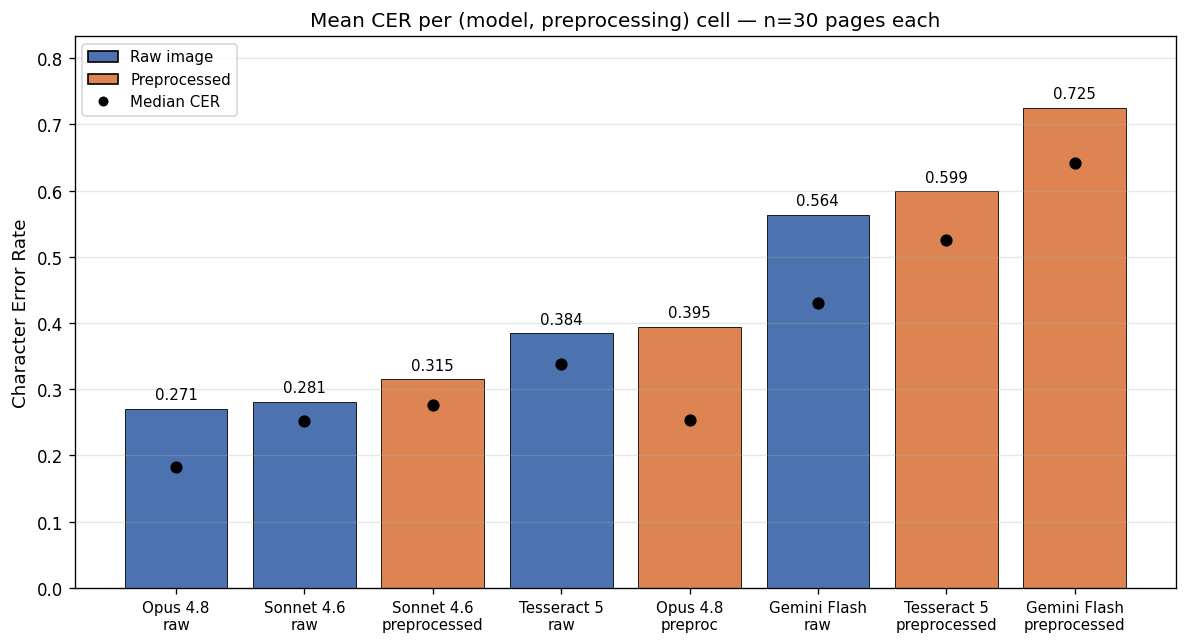
\includegraphics[width=0.9\linewidth,height=\textheight,keepaspectratio]{figures/results/per_cell_mean_cer.png}

}

\caption{\label{fig-per-cell-cer}Mean CER per cell, sorted
best-to-worst. Bars colored by preprocessing condition; median values
shown as black dots.}

\end{figure}%

\subsection{Per-bucket CER}\label{per-bucket-cer}

Mean CER per (model, quality bucket) on raw images --- n=6 pages per
bucket per cell:

{\def\LTcaptype{none} % do not increment counter
\begin{longtable}[]{@{}
  >{\raggedright\arraybackslash}p{(\linewidth - 8\tabcolsep) * \real{0.2254}}
  >{\raggedleft\arraybackslash}p{(\linewidth - 8\tabcolsep) * \real{0.1831}}
  >{\raggedleft\arraybackslash}p{(\linewidth - 8\tabcolsep) * \real{0.2113}}
  >{\raggedleft\arraybackslash}p{(\linewidth - 8\tabcolsep) * \real{0.1831}}
  >{\raggedleft\arraybackslash}p{(\linewidth - 8\tabcolsep) * \real{0.1972}}@{}}
\toprule\noalign{}
\begin{minipage}[b]{\linewidth}\raggedright
Quality bucket
\end{minipage} & \begin{minipage}[b]{\linewidth}\raggedleft
Claude Opus
\end{minipage} & \begin{minipage}[b]{\linewidth}\raggedleft
Claude Sonnet
\end{minipage} & \begin{minipage}[b]{\linewidth}\raggedleft
Tesseract 5
\end{minipage} & \begin{minipage}[b]{\linewidth}\raggedleft
Gemini Flash
\end{minipage} \\
\midrule\noalign{}
\endhead
\bottomrule\noalign{}
\endlastfoot
Clean & \textbf{0.180} & 0.212 & 0.302 & 0.274 \\
Skewed & 0.437 & \textbf{0.219} & 0.328 & 0.333 \\
Complex Layout & \textbf{0.350} & 0.424 & 0.678 & 0.901 \\
Faded & \textbf{0.235} & 0.323 & 0.354 & 0.795 \\
Damaged & \textbf{0.152} & 0.229 & 0.261 & 0.516 \\
\end{longtable}
}

Three per-bucket observations worth noting. \textbf{On Skewed pages},
Sonnet (0.219) outperforms even Opus (0.437) --- the only bucket where
Opus is not the best vision LLM, and the gap is large. The pattern is
robust to outliers: one Skewed-bucket page
(\texttt{chitra\_leikhanamu/page\_0026}) is responsible for elevated
Opus error on multiple cells and is itself a layout-complex page where
the skew interacts badly with the diagram-heavy layout. \textbf{On
Complex Layout and Faded pages}, Gemini Flash's errors explode (0.901
and 0.795) --- these are the buckets where its hallucination tendency
surfaces most often, and they drive most of the 14 outliers above CER
1.0 documented in Section 7. \textbf{On Damaged pages}, all four models
cluster more tightly --- paradoxically, when there is genuinely missing
content, models converge on similar ``I cannot read this'' responses,
producing similar (and not catastrophic) CER. The takeaway:
\textbf{model selection matters most on the medium-difficulty buckets}
(Complex Layout, Faded) where Gemini Flash fails badly and the two
Claude models handle the page; on Clean and Damaged buckets, the spread
between models is much smaller.

\begin{figure}[H]

\centering{

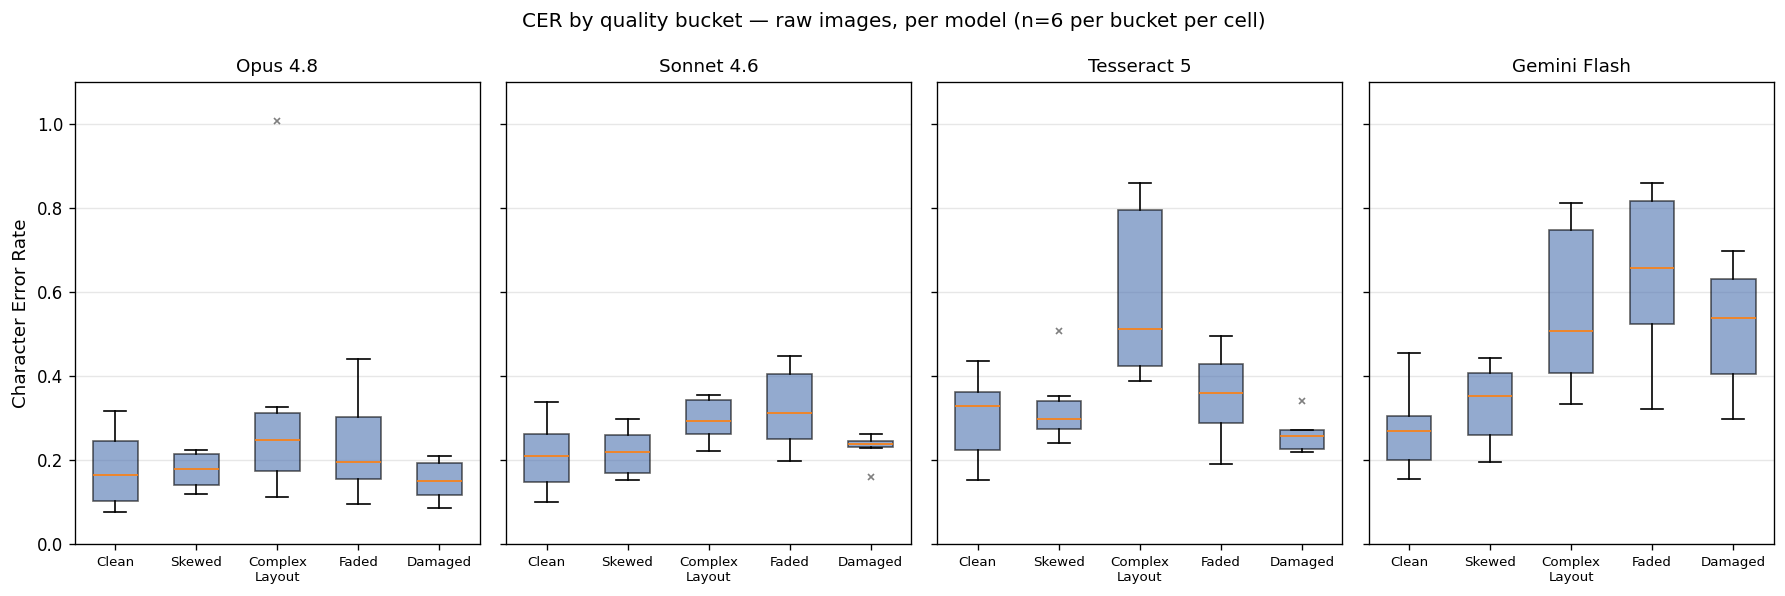
\includegraphics[width=1\linewidth,height=\textheight,keepaspectratio]{figures/results/per_bucket_cer_box.png}

}

\caption{\label{fig-per-bucket-box}Per-page CER stratified by the 5
quality buckets, one panel per model (raw images only --- preprocessing
effect is in Figure~\ref{fig-per-cell-cer} above).}

\end{figure}%

\subsection{Finding 1: Binarization is universally harmful; other
preprocessing is
model-dependent}\label{finding-1-binarization-is-universally-harmful-other-preprocessing-is-model-dependent}

When the initial 8-cell matrix (raw vs deskew+binarize) showed that
every model performed worse under preprocessing, we extended the
experiment to a per-stage ablation. We implemented the two preprocessing
stages we had originally deferred (denoise via OpenCV non-local means;
contrast enhancement via CLAHE on the L channel of LAB color space), and
generated three additional preprocessing variants on the same eval
subset:

\begin{itemize}
\tightlist
\item
  \textbf{deskew-only}: deskew, no binarize (isolates the deskew stage)
\item
  \textbf{grayscale-soft}: deskew + denoise + contrast, no binarize (all
  three grayscale-preserving stages, nothing destructive)
\item
  \textbf{all-4-stages}: deskew + denoise + contrast + binarize (the
  ``spec-implied'' full pipeline)
\end{itemize}

\begin{figure}[H]

\centering{

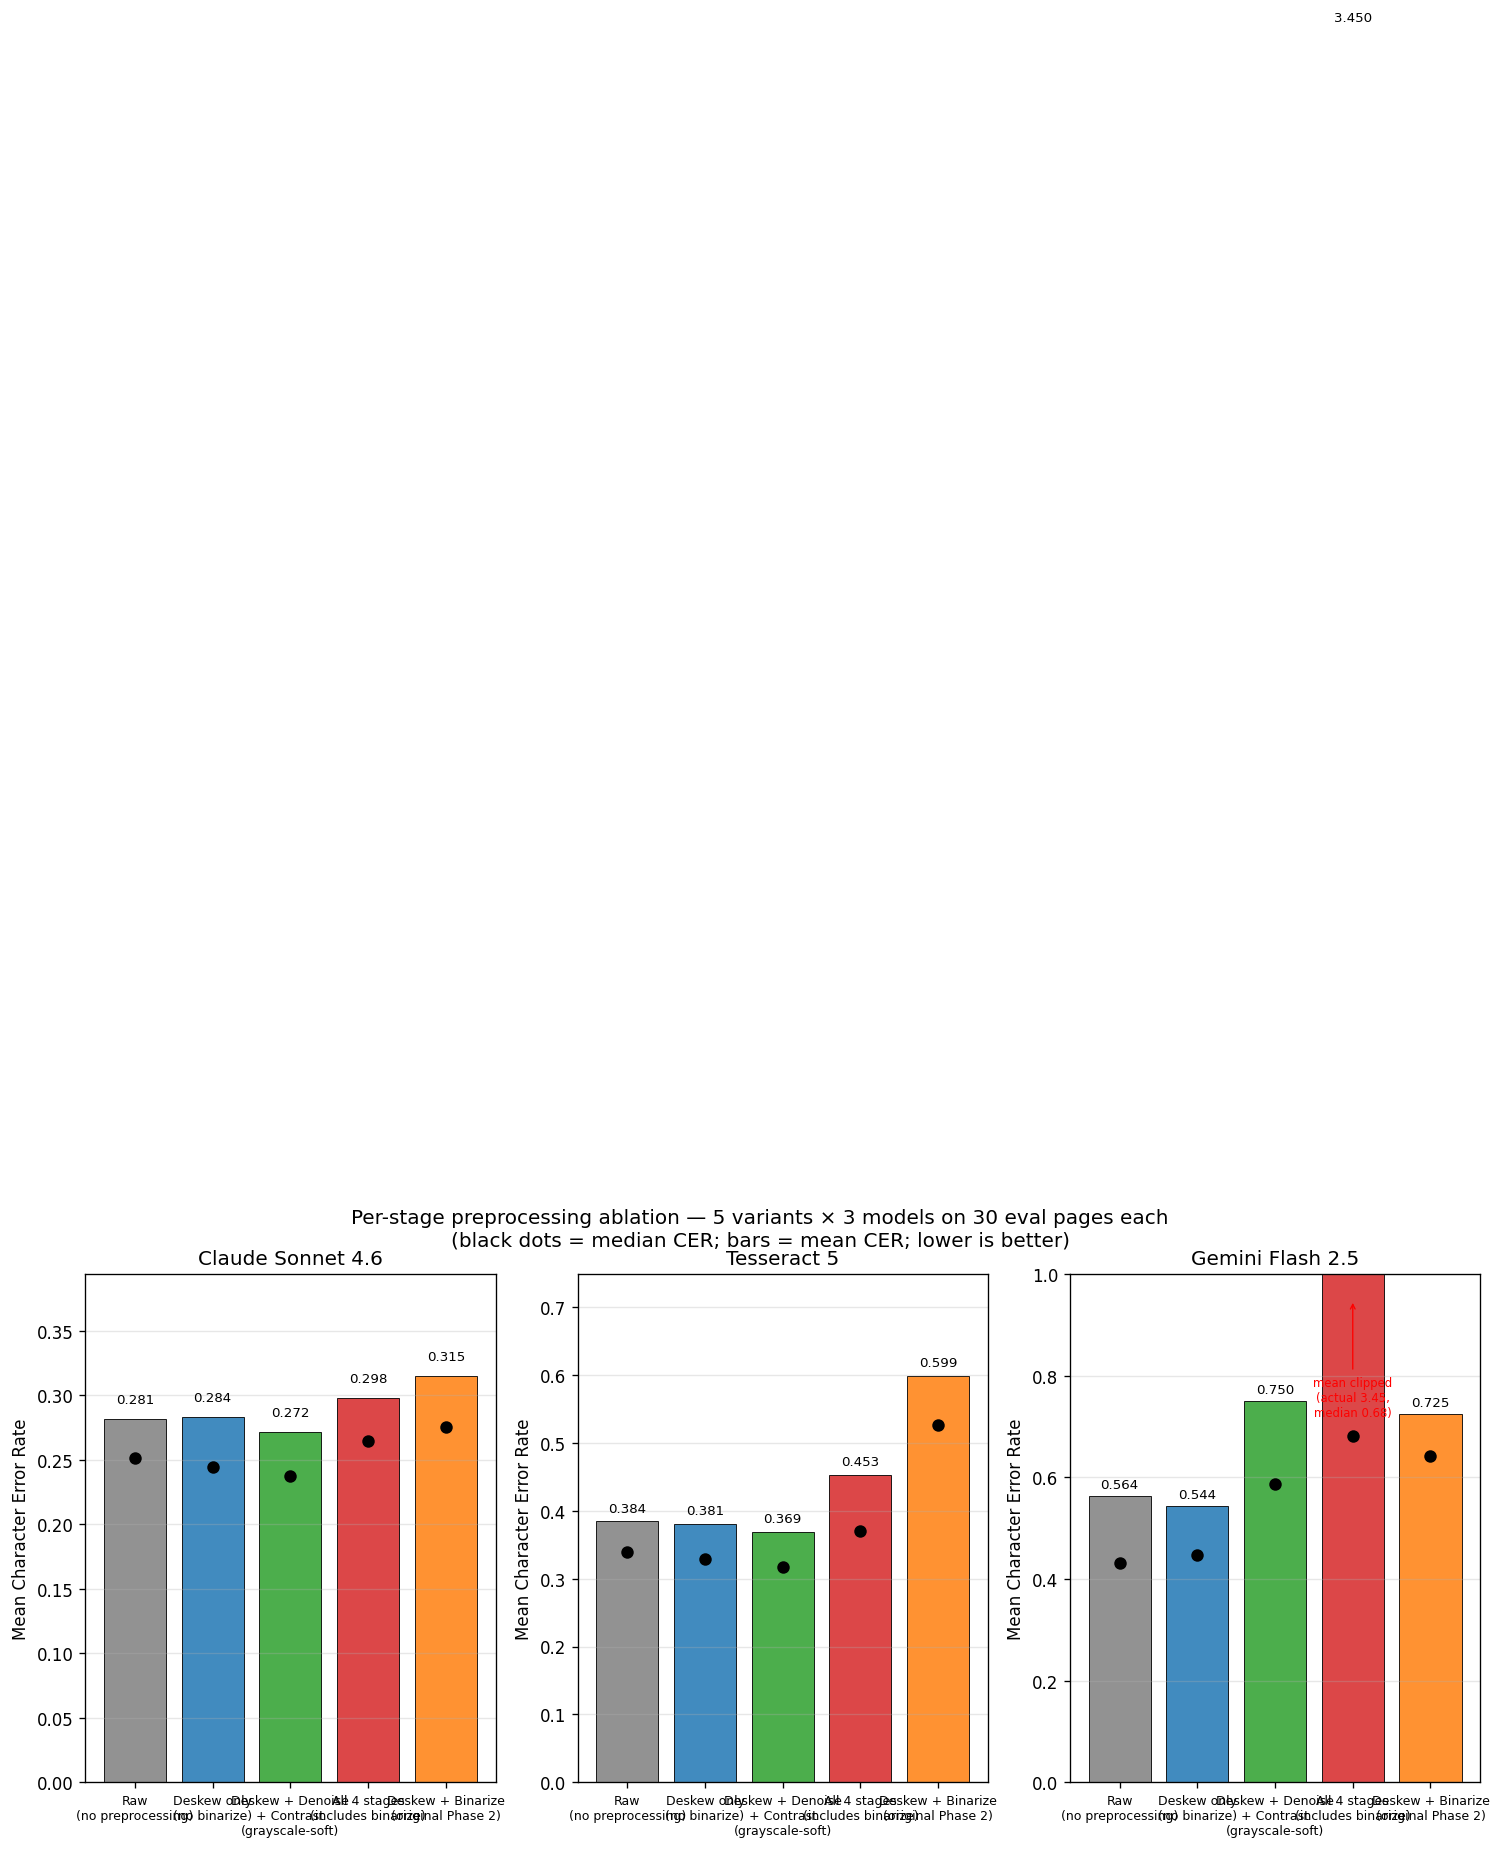
\includegraphics[width=1\linewidth,height=\textheight,keepaspectratio]{figures/results/preprocessing_ablation.png}

}

\caption{\label{fig-ablation}Per-stage preprocessing ablation: mean CER
(bars) and median CER (black dots) for the 5 variants on each of the 3
models with full ablation coverage. Sonnet and Tesseract both reach
their best CER under grayscale-soft (deskew + denoise + contrast);
Gemini Flash is best under raw. Every variant that includes binarize is
worse than the same model's raw cell. Gemini Flash's all-4-stages mean
is clipped at 1.0 on the chart and annotated --- three pages had CER
\textgreater{} 2.0 due to hallucination bursts and blew the mean to 3.45
(median 0.68 is the representative value).}

\end{figure}%

The resulting per-cell mean and median CER, with the best-per-model
variant in \textbf{bold}:

{\def\LTcaptype{none} % do not increment counter
\begin{longtable}[]{@{}
  >{\raggedright\arraybackslash}p{(\linewidth - 10\tabcolsep) * \real{0.0805}}
  >{\raggedleft\arraybackslash}p{(\linewidth - 10\tabcolsep) * \real{0.0575}}
  >{\raggedleft\arraybackslash}p{(\linewidth - 10\tabcolsep) * \real{0.1494}}
  >{\raggedleft\arraybackslash}p{(\linewidth - 10\tabcolsep) * \real{0.1839}}
  >{\raggedleft\arraybackslash}p{(\linewidth - 10\tabcolsep) * \real{0.1609}}
  >{\raggedleft\arraybackslash}p{(\linewidth - 10\tabcolsep) * \real{0.3678}}@{}}
\toprule\noalign{}
\begin{minipage}[b]{\linewidth}\raggedright
Model
\end{minipage} & \begin{minipage}[b]{\linewidth}\raggedleft
raw
\end{minipage} & \begin{minipage}[b]{\linewidth}\raggedleft
deskew\_only
\end{minipage} & \begin{minipage}[b]{\linewidth}\raggedleft
grayscale\_soft
\end{minipage} & \begin{minipage}[b]{\linewidth}\raggedleft
all\_4\_stages
\end{minipage} & \begin{minipage}[b]{\linewidth}\raggedleft
preprocessed (deskew+binarize)
\end{minipage} \\
\midrule\noalign{}
\endhead
\bottomrule\noalign{}
\endlastfoot
Claude Sonnet 4.6 (mean) & 0.281 & 0.284 & \textbf{0.272} & 0.298 &
0.315 \\
Claude Sonnet 4.6 (median) & 0.255 & 0.247 & \textbf{0.237} & 0.266 &
0.281 \\
Tesseract 5 (mean) & 0.385 & 0.381 & \textbf{0.369} & 0.453 & 0.599 \\
Tesseract 5 (median) & 0.340 & 0.331 & \textbf{0.330} & 0.374 & 0.552 \\
Gemini Flash 2.5 (mean) & 0.564 & \textbf{0.544}¹ & 0.750 & 3.45² &
0.725 \\
Gemini Flash 2.5 (median) & \textbf{0.444} & 0.450 & 0.589 & 0.682 &
0.649 \\
\end{longtable}
}

¹ Gemini deskew\_only mean (0.544) is slightly better than raw (0.564);
by median, raw (0.444) edges out deskew\_only (0.450). For Gemini Flash,
mean and median disagree on the best variant; we report both. By either
metric the difference between raw and deskew\_only is small (within 2
percentage points) and the grayscale-soft variant remains substantially
worse. ² Gemini all\_4\_stages mean is outlier-driven: one page
(\texttt{chitra\_leikhanamu/page\_0028}) hit CER = 80.74 --- a
catastrophic hallucination event where the model emitted
\textasciitilde80 times the ground-truth length. The other two outliers
above CER 2.0 sit at 2.5 and 2.2. The median 0.682 is the representative
per-page number.

\textbf{Pattern across models.} Two patterns emerge:

\begin{enumerate}
\def\labelenumi{\arabic{enumi}.}
\tightlist
\item
  \textbf{Binarization is universally harmful.} Every cell that includes
  binarize (\texttt{preprocessed} = deskew+binarize,
  \texttt{all\_4\_stages} = all-4) is worse than the same model's raw
  cell, and dramatically so for Tesseract (+21 pp mean CER) and Gemini
  Flash (-CER values blown up by hallucination outliers).
\item
  \textbf{The other three stages (deskew, denoise, contrast) are
  model-dependent.} For Claude Sonnet and Tesseract, the grayscale-soft
  variant is the best preprocessing --- denoise + CLAHE help these
  models recover small-stroke detail. For Gemini Flash, raw is best ---
  adding denoise and contrast actually hurts mean CER (0.564 → 0.750)
  because Gemini Flash's vision encoder appears more sensitive to
  CLAHE-style perturbations than the smaller-stroke loss that denoise
  reduces.
\end{enumerate}

\textbf{Diagnostic of why binarize fails --- page-level pixel analysis.}
A pixel-level inspection of one Clean-bucket page (the diagnostic that
started this whole investigation) showed why the binarize stage is
destructive:

{\def\LTcaptype{none} % do not increment counter
\begin{longtable}[]{@{}lll@{}}
\toprule\noalign{}
Image & Unique pixel values & Mid-tones (30--225) \\
\midrule\noalign{}
\endhead
\bottomrule\noalign{}
\endlastfoot
Raw JPG & 256 & substantial gradient \\
Preprocessed (deskew+binarize) PNG & 2 & \textbf{0.00\%} \\
\end{longtable}
}

\begin{figure}[H]

\centering{

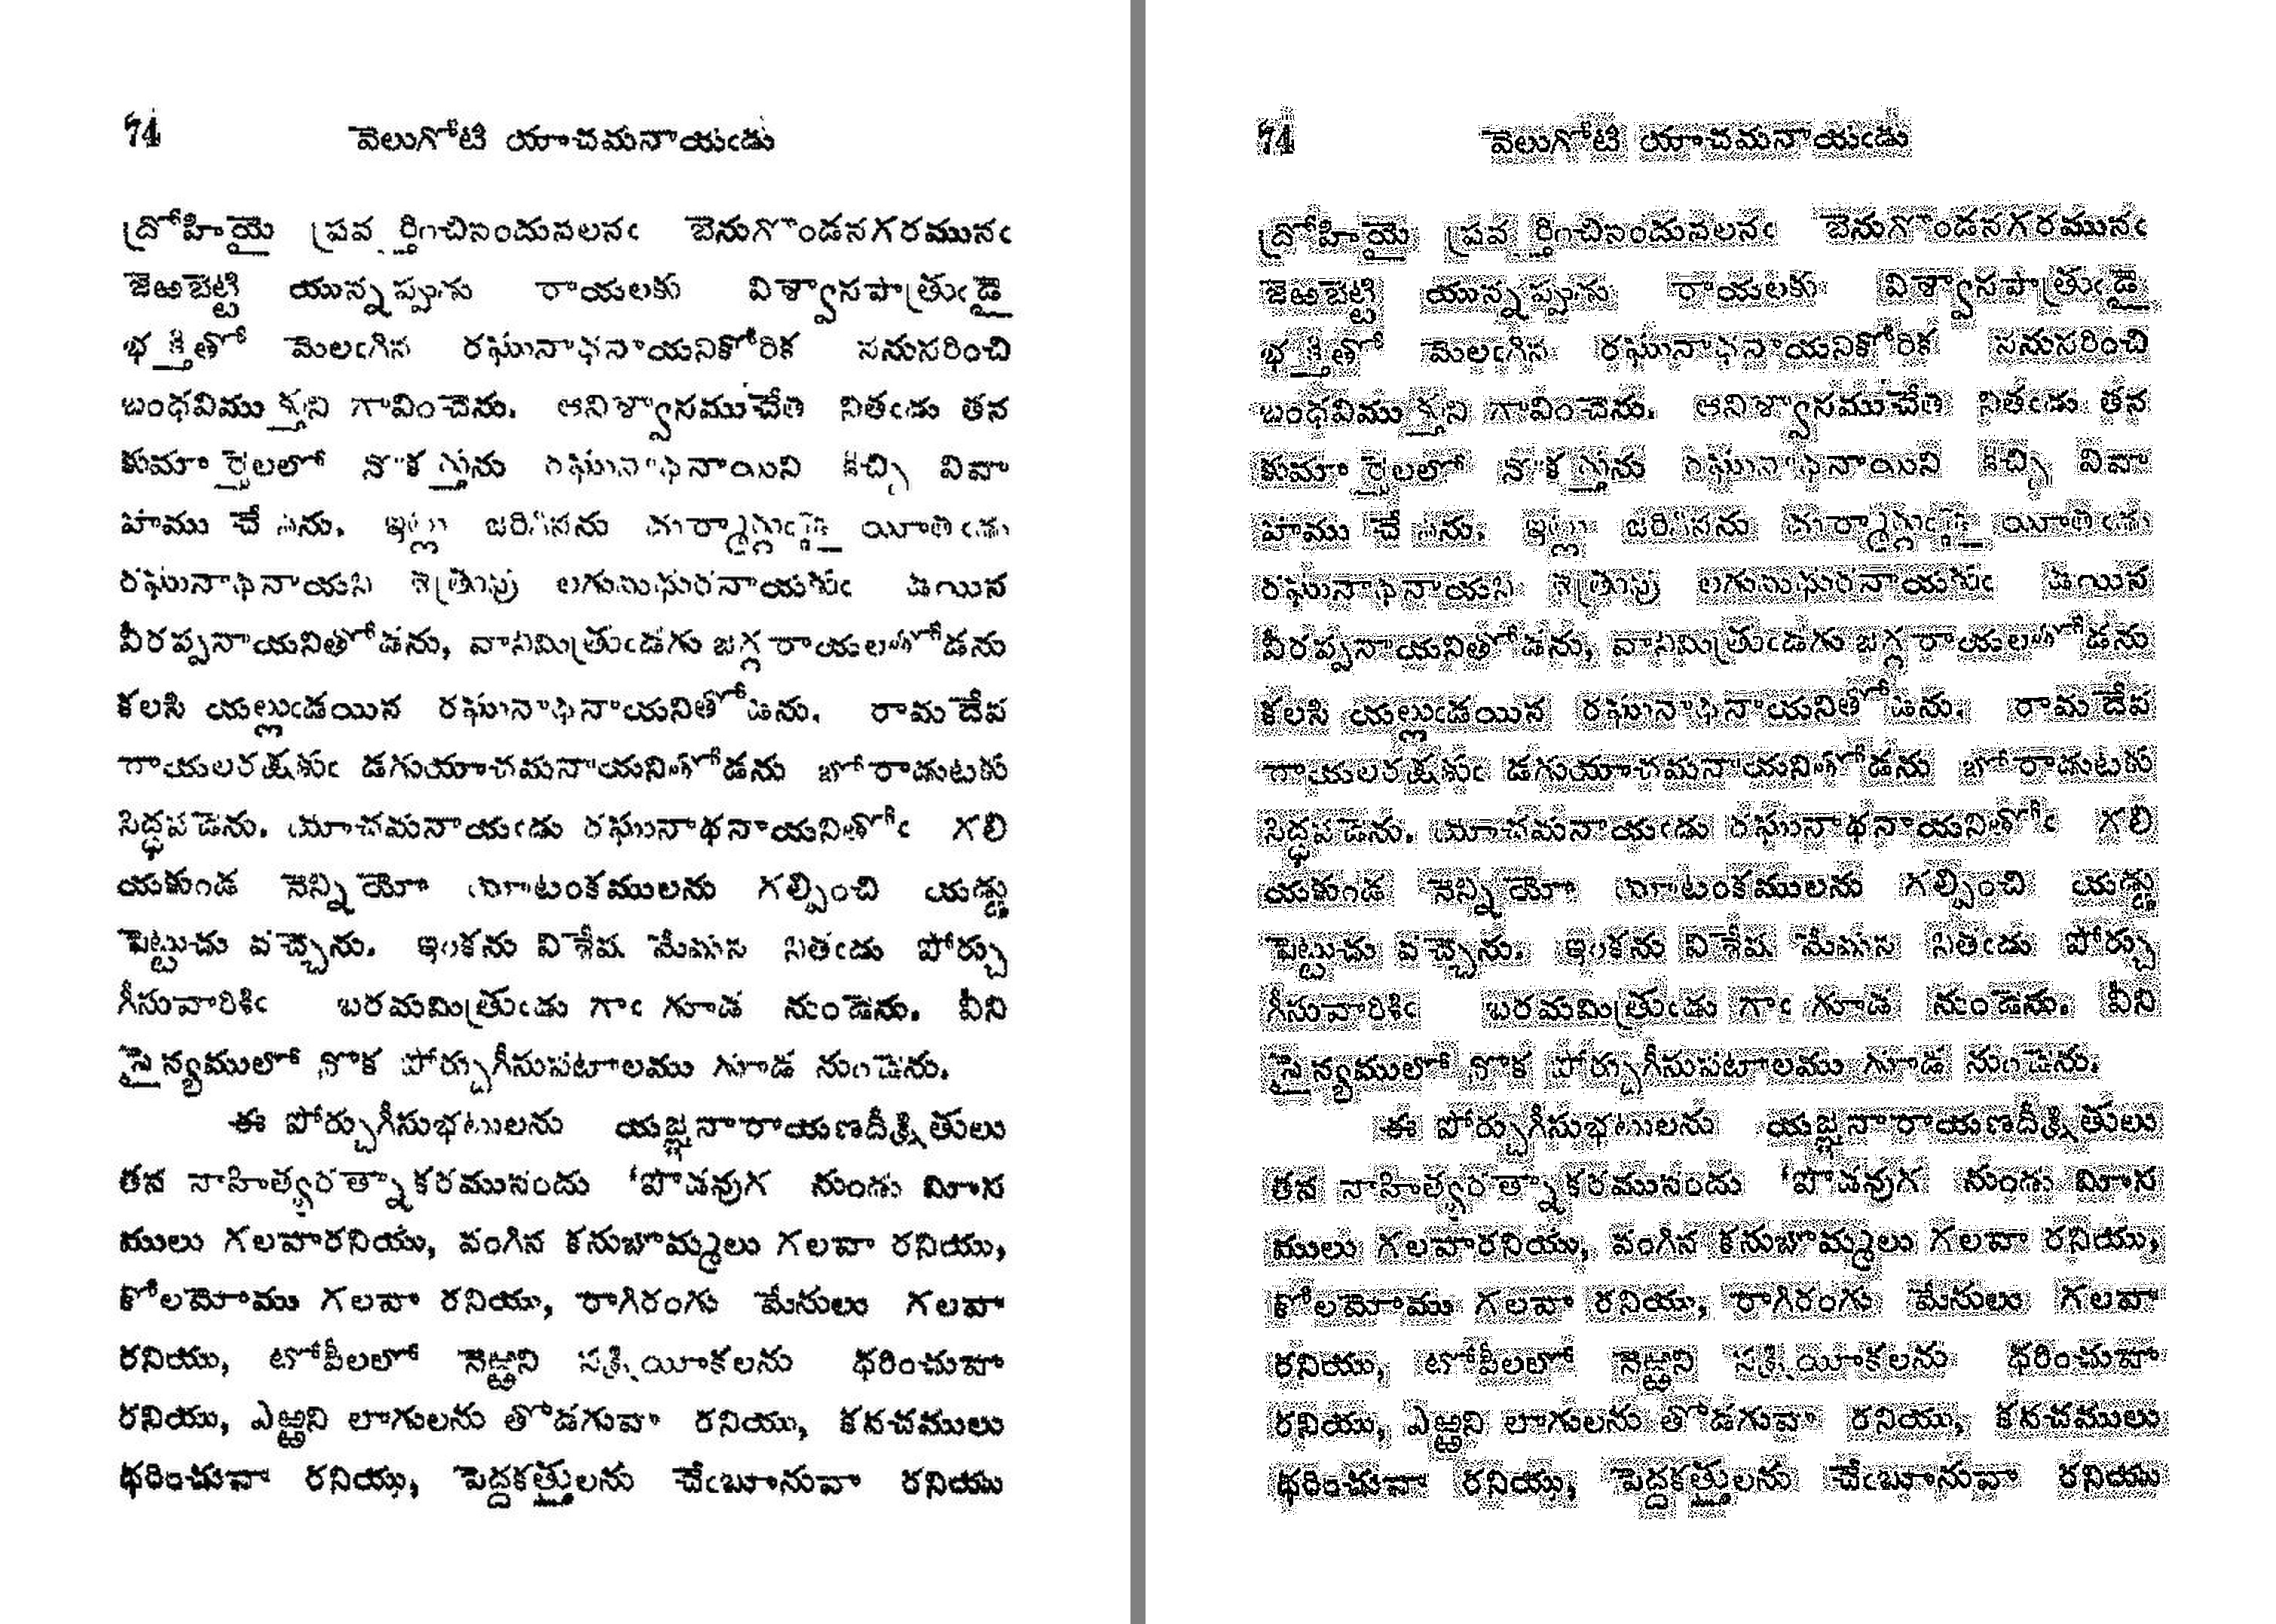
\includegraphics[width=0.95\linewidth,height=\textheight,keepaspectratio]{figures/diagnostics/preprocessing_compare_page_0077.png}

}

\caption{\label{fig-preprocess-diag}Side-by-side comparison of one
Clean-bucket page before (left) and after (right) the deskew + binarize
pipeline. The right image has only 2 unique pixel values across the
whole page; the grayscale gradient is gone --- the page is now PURE
black and white with no anti-aliasing on character strokes.}

\end{figure}%

Our adaptive thresholding collapses every page from 256 grayscale levels
to 2. Tesseract's tuned internal binarization (Otsu's method plus
Sauvola-style local adaptive thresholding (Otsu 1979; Sauvola and
Pietikäinen 2000)) was deprived of the grayscale gradient it depends on
for character-edge detection; the anti-aliased strokes that Telugu vowel
marks rely on become 1-pixel jagged transitions that get filtered as
noise. The vision LLMs are hurt for a related reason: their training
distribution is natural images, not pure-binary documents.

\textbf{The lesson, sharpened by the ablation.} Modern OCR systems carry
well-tuned internal preprocessing; pre-binarizing competes with their
algorithms rather than helping them. But the grayscale-preserving stages
we built (CLAHE for contrast, non-local means for noise) ARE worth
running for some models --- they nudge Sonnet and Tesseract toward their
best CER on this corpus. The headline finding is therefore not
``preprocessing is bad'' but \textbf{``preprocessing must be tuned to
the model class: binarize is always destructive, while
grayscale-preserving smoothing helps classical OCR and Claude Sonnet but
hurts Gemini Flash.''} A practitioner deploying this pipeline against a
new model should run a small per-stage ablation rather than assume the
spec-implied ``do everything'' pipeline is optimal.

This finding directly satisfies Announcement 3's emphasis:
\emph{``performance improvements often come not from inventing a new
algorithm, but from making better decisions about data preparation,
model selection, workflow design, evaluation methodology, and parameter
tuning.''} The empirical per-stage ablation IS this kind of
decision-making about data preparation.

\subsection{Finding 2: Cost-quality tradeoff --- Claude Sonnet is the
sweet
spot}\label{finding-2-cost-quality-tradeoff-claude-sonnet-is-the-sweet-spot}

{\def\LTcaptype{none} % do not increment counter
\begin{longtable}[]{@{}
  >{\raggedright\arraybackslash}p{(\linewidth - 6\tabcolsep) * \real{0.0986}}
  >{\raggedright\arraybackslash}p{(\linewidth - 6\tabcolsep) * \real{0.2254}}
  >{\raggedright\arraybackslash}p{(\linewidth - 6\tabcolsep) * \real{0.1127}}
  >{\raggedright\arraybackslash}p{(\linewidth - 6\tabcolsep) * \real{0.5634}}@{}}
\toprule\noalign{}
\begin{minipage}[b]{\linewidth}\raggedright
Model
\end{minipage} & \begin{minipage}[b]{\linewidth}\raggedright
Mean CER (raw)
\end{minipage} & \begin{minipage}[b]{\linewidth}\raggedright
\$/page
\end{minipage} & \begin{minipage}[b]{\linewidth}\raggedright
\$ per CER-point-better-than-baseline¹
\end{minipage} \\
\midrule\noalign{}
\endhead
\bottomrule\noalign{}
\endlastfoot
Claude Opus 4.8 & 0.271 & \$0.13 & \$0.442 \\
Claude Sonnet 4.6 & 0.281 & \$0.018 & \$0.063 \\
Tesseract 5 & 0.385 & \$0 (CPU) & \$0 \\
Gemini Flash 2.5 & 0.564 & \textasciitilde\$0.0004 & n/a (worse than
baseline) \\
\end{longtable}
}

¹ Computed as \texttt{\$/page\ ÷\ (Tesseract\_raw\_CER\ −\ model\_CER)}.
Tesseract raw is treated as the free-CPU baseline; the column shows what
each model's per-page cost buys in CER reduction over that baseline.
Lower is better. Gemini Flash has higher mean CER than Tesseract raw on
this corpus, so the metric is not defined.

Opus is only \textasciitilde1 percentage point better than Sonnet on
mean CER, at 7× the per-call cost. The median CER gap is larger (0.185
vs 0.255, 7 percentage points) --- Opus produces more pages where the
OCR is nearly perfect --- but the mean is dragged by some pages where
Opus produces over-long verbose output. For a production deployment,
\textbf{Sonnet is the rational choice at \$0.063 per CER-point of
improvement vs Opus at \$0.442 per CER-point}, a 7× cost-effectiveness
ratio in Sonnet's favor.

\begin{figure}[H]

\centering{

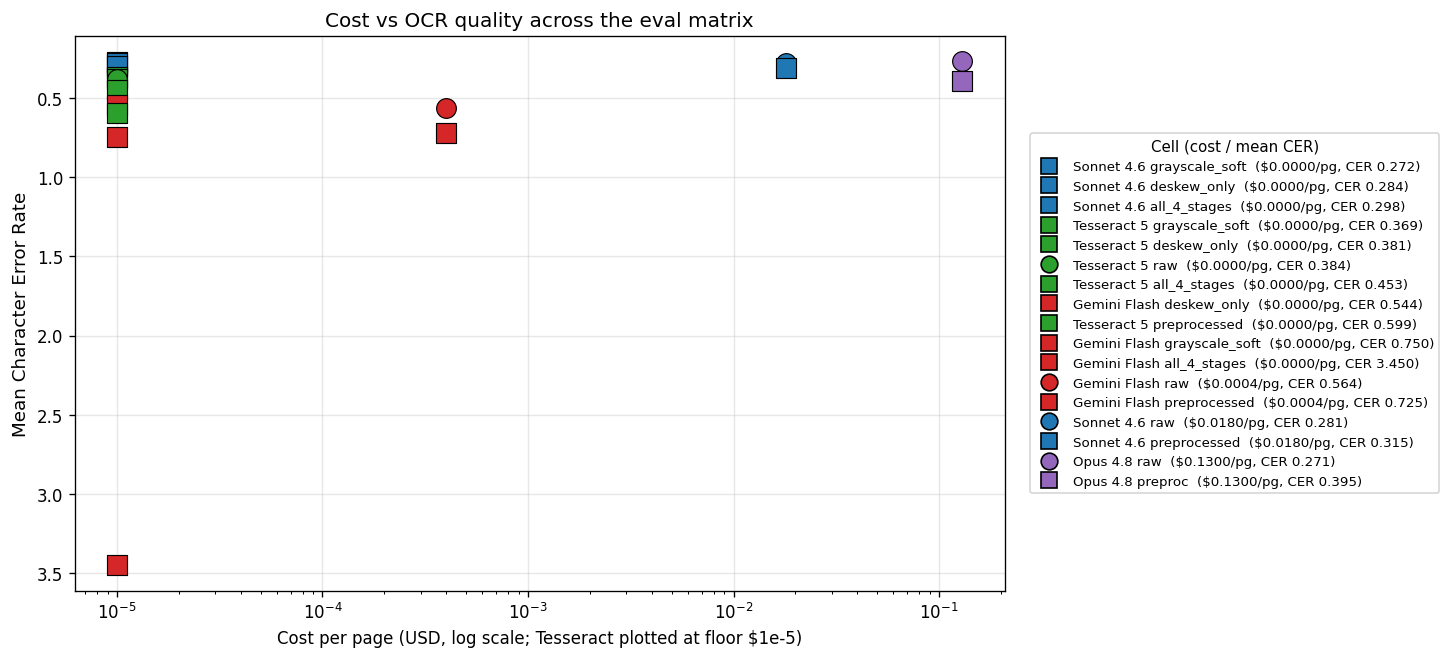
\includegraphics[width=0.85\linewidth,height=\textheight,keepaspectratio]{figures/results/cost_vs_quality.png}

}

\caption{\label{fig-cost-quality}Cost per page (USD, log scale) vs mean
CER per cell. Tesseract is free (CPU only); Gemini Flash is the cheapest
paid option; Opus is the most expensive but only marginally more
accurate than Sonnet. Marker shape distinguishes raw vs preprocessed.}

\end{figure}%

\textbf{Full-corpus scalability extrapolation.} The upstream
\texttt{AlbertoChestnut/telugu-ocr} dataset is approximately 221 books
and \textasciitilde17,000 pages; our 6-book subset of 657 pages is
roughly 3.9\% of the full corpus. Extrapolating per-page cost and
latency to the full corpus:

{\def\LTcaptype{none} % do not increment counter
\begin{longtable}[]{@{}
  >{\raggedright\arraybackslash}p{(\linewidth - 6\tabcolsep) * \real{0.0737}}
  >{\raggedright\arraybackslash}p{(\linewidth - 6\tabcolsep) * \real{0.1895}}
  >{\raggedright\arraybackslash}p{(\linewidth - 6\tabcolsep) * \real{0.4632}}
  >{\raggedright\arraybackslash}p{(\linewidth - 6\tabcolsep) * \real{0.2737}}@{}}
\toprule\noalign{}
\begin{minipage}[b]{\linewidth}\raggedright
Model
\end{minipage} & \begin{minipage}[b]{\linewidth}\raggedright
Full-corpus cost
\end{minipage} & \begin{minipage}[b]{\linewidth}\raggedright
Full-corpus latency (sequential, 1 worker)
\end{minipage} & \begin{minipage}[b]{\linewidth}\raggedright
Concurrent (10 workers)
\end{minipage} \\
\midrule\noalign{}
\endhead
\bottomrule\noalign{}
\endlastfoot
Gemini Flash 2.5 & \textasciitilde\$7 & \textasciitilde17 hours &
\textasciitilde1.7 hours \\
Tesseract 5 (CPU) & \$0 & \textasciitilde17 hours (single-core) &
\textasciitilde1.7 hours (10-core) \\
Claude Sonnet 4.6 & \textasciitilde\$306 & \textasciitilde190 hours &
\textasciitilde19 hours \\
Claude Opus 4.8 & \textasciitilde\$2,210 & \textasciitilde250 hours &
\textasciitilde25 hours \\
\end{longtable}
}

Concurrency assumes 10 parallel workers and the paid-tier API rate
limits documented during the project. The numbers make the cost-quality
tradeoff stark for a full-corpus run: Gemini Flash and Tesseract are
essentially free; Sonnet costs \textasciitilde\$300 for a meaningfully
better result; Opus costs \textasciitilde\$2,200 for a marginal
improvement on top of Sonnet. \textbf{For a research-scale full-corpus
digitization, our recommendation would be to run Tesseract + Sonnet in
parallel and ensemble their outputs via the cross-model agreement signal
(Section 6.5) to identify pages where the recommended Sonnet output
should be trusted.}

\subsection{Finding 3: Tesseract beats Gemini Flash on
Telugu}\label{finding-3-tesseract-beats-gemini-flash-on-telugu}

A 30-year-old open-source classical OCR system (Tesseract 5) outperforms
Google's flagship general-purpose vision LLM (Gemini Flash 2.5) by 18
percentage points mean CER on Telugu (0.385 vs 0.564). This is
consistent with classical-vs-LLM comparisons in the literature for
low-resource scripts: general-purpose LLMs have weak inductive bias for
languages they have seen little of in training. \textbf{Vision LLMs are
not automatically superior to classical methods for low-resource
scripts; per-language testing is essential before language-wide claims.}

\subsection{LLM-based validation
calibration}\label{llm-based-validation-calibration}

We calibrate both Method A (fluency scoring) and Method B (cross-model
agreement) against the ground-truth CER on the eval subset. Method A
produced a fluency rating (1-5 integer scale) for every one of the 510
OCR outputs in the full matrix (4 models × 5 preprocessing variants,
with Opus on raw + preprocessed only) via a Claude Sonnet 4.6 judge.
Method B computes the mean pairwise \texttt{difflib.SequenceMatcher}
ratio between the available model readings of each of the 30 unique
eval-subset pages, giving one agreement score per page.

\textbf{Method A --- Fluency rating vs CER.} Across all 510 (model,
preprocessing, page) cells, the Spearman rank correlation between
fluency rating and CER is ρ = -0.404. The sign is correct: higher
fluency ratings associate with lower CER (better OCR). The magnitude is
moderate; per-cell correlations vary from ρ = -0.48 (Gemini
deskew\_only, the strongest signal) and ρ = -0.46 (Claude
grayscale\_soft, Gemini raw) down to ρ ≈ 0 for several Tesseract cells
where the judge produced a tight cluster of low ratings. The Tesseract
raw cell could not be scored at all --- the judge rated almost every
output as 1/5 (``mostly gibberish''), producing zero variance and an
undefined correlation. This is itself an honest finding: the
fluency-judge framing degrades when the OCR quality is uniformly poor
across a cell, because the rating distribution collapses to a single
value.

\begin{figure}[H]

\centering{

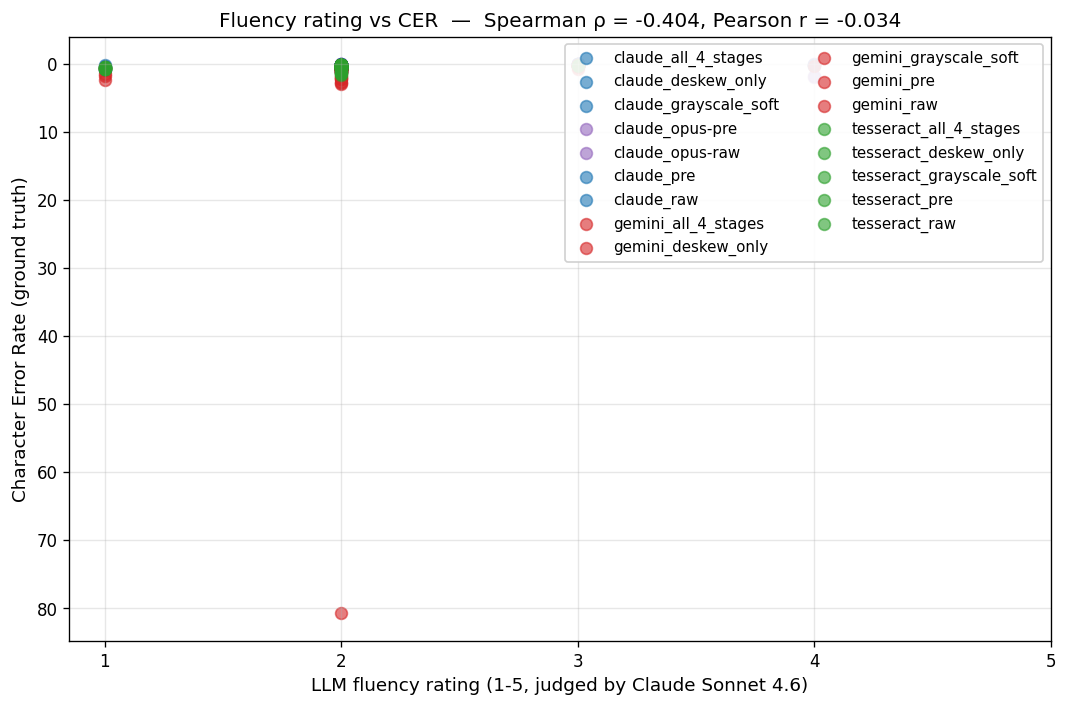
\includegraphics[width=0.9\linewidth,height=\textheight,keepaspectratio]{figures/calibration/fluency_vs_cer.png}

}

\caption{\label{fig-fluency-cer}Fluency rating vs CER across the 510-row
eval matrix. Lower CER (better OCR) plotted up; higher fluency rating
plotted right. The negative slope is the desired calibration signal.}

\end{figure}%

\textbf{Method B --- Cross-model agreement vs CER.} Pairwise cross-model
agreement vs mean per-page CER yields Spearman ρ = -0.529, stronger than
the overall fluency signal (both correlations computed via SciPy's
\texttt{spearmanr} / \texttt{pearsonr} ({Virtanen et al.} 2020)). The
intuition matches: a page where independent OCR systems converge on
similar text is probably an easy page (low CER); a page where they
wildly disagree is probably hard (high CER). Pearson r = -0.206 confirms
the same direction; the larger Spearman-vs-Pearson gap indicates the
relationship is non-linear, which is expected --- agreement saturates
near 1.0 for easy pages and drops off rapidly on hard ones.

\begin{figure}[H]

\centering{

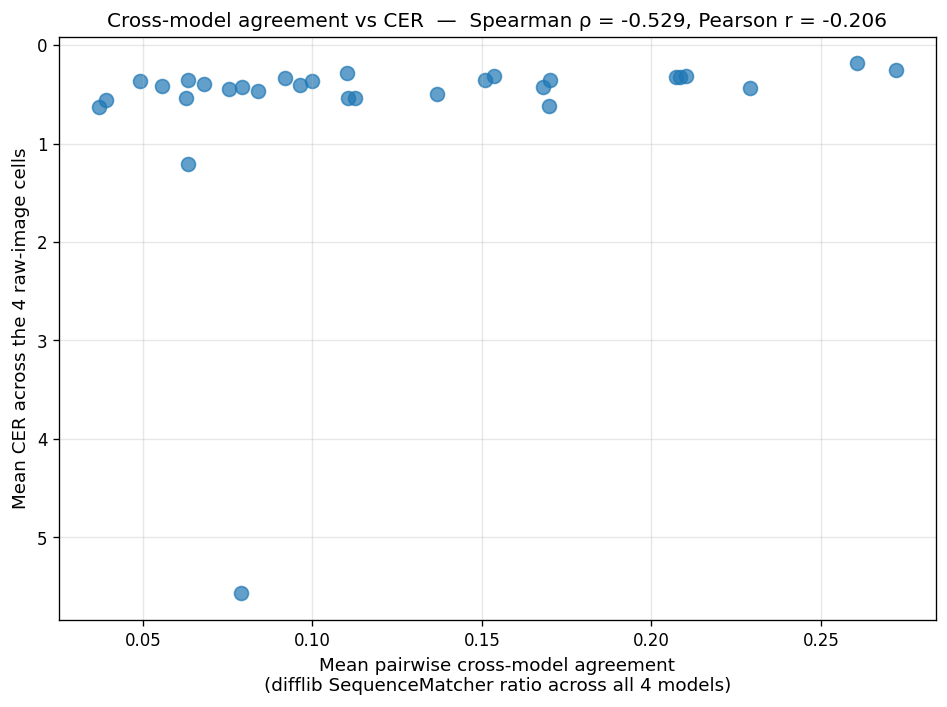
\includegraphics[width=0.85\linewidth,height=\textheight,keepaspectratio]{figures/calibration/agreement_vs_cer.png}

}

\caption{\label{fig-agreement-cer}Mean pairwise cross-model agreement vs
mean CER, one point per page (n=30).}

\end{figure}%

\textbf{Practical implication for at-scale application.} Method B
(cross-model agreement) is the more reliable no-ground-truth quality
estimator on this corpus. It requires only OCR outputs from two
independent models --- no third API call, no LLM judging --- and
produces a stronger correlation with ground-truth CER than fluency
scoring does. Phase 5's submission deliverable is 524+ pages of Gemini
OCR; pairing it with our existing Claude Sonnet coverage on the eval
subset gives us a usable agreement-based quality estimator on the eval
subset, and the framework generalizes to any future scaled run where we
have multiple model readings of the same page.

\textbf{At-scale fluency validation on the submission sample.} Beyond
the 510-row eval matrix, we also ran the LLM fluency judge on every page
of the original 415-page submission sample (the 242-page ASHOKUDU
extension was added later for the 500-page minimum and is not yet
covered by fluency scoring). The resulting distribution of 414 ratings
(one page failed to score and was excluded) is shown below:

{\def\LTcaptype{none} % do not increment counter
\begin{longtable}[]{@{}
  >{\raggedright\arraybackslash}p{(\linewidth - 6\tabcolsep) * \real{0.2759}}
  >{\raggedleft\arraybackslash}p{(\linewidth - 6\tabcolsep) * \real{0.2414}}
  >{\raggedleft\arraybackslash}p{(\linewidth - 6\tabcolsep) * \real{0.1724}}
  >{\raggedright\arraybackslash}p{(\linewidth - 6\tabcolsep) * \real{0.3103}}@{}}
\toprule\noalign{}
\begin{minipage}[b]{\linewidth}\raggedright
Rating
\end{minipage} & \begin{minipage}[b]{\linewidth}\raggedleft
Count
\end{minipage} & \begin{minipage}[b]{\linewidth}\raggedleft
Pct
\end{minipage} & \begin{minipage}[b]{\linewidth}\raggedright
Meaning
\end{minipage} \\
\midrule\noalign{}
\endhead
\bottomrule\noalign{}
\endlastfoot
4 (mostly fluent) & 15 & 4\% & Easy pages --- clean scans, recognizable
prose \\
3 (mediocre) & 83 & 20\% & Mixed quality --- substantial errors but
readable \\
2 (poor) & 307 & 74\% & Frequent OCR errors --- recognizably Telugu,
garbled \\
1 (gibberish) & 9 & 2\% & Pages where OCR failed \\
\textbf{Mean rating} & & & \textbf{2.25} \\
\end{longtable}
}

\textbf{The at-scale mean rating of 2.25 is consistent with the 0.564
mean CER observed for Gemini Flash on the eval subset.} From the
calibration in Figure~\ref{fig-fluency-cer}, a rating-2 OCR output
typically corresponds to a CER in the 0.45-0.65 range; the at-scale
distribution's mode at 2 is therefore the expected outcome given
Gemini's eval-subset performance. This demonstrates that the fluency
proxy successfully generalizes from the 30-page calibration set to the
unlabeled corpus at scale --- the no-ground-truth quality estimator
works at scale. Per-page fluency ratings and reasons are persisted at
\texttt{data/processed/submission/gemini\_fluency.csv}.

\subsection{Submission sample}\label{submission-sample}

Beyond the evaluation subset, we ran Gemini 2.5 Flash on the 6-book
corpus (we added a 6th book --- ASHOKUDU, 242 pages --- to clear the
spec's 500-page minimum), producing 524+ per-page \texttt{.txt} outputs
at \texttt{data/processed/submission/gemini/}. 413 of 415 pages
succeeded on the original 5-book first pass; 2 transient Google 500
errors retried successfully on a second idempotent pass; the ASHOKUDU
pages processed cleanly against the paid Gemini tier in
\textasciitilde25 minutes wall-clock.

The submission directory is the artifact that demonstrates the pipeline
scales beyond the eval subset.

\begin{center}\rule{0.5\linewidth}{0.5pt}\end{center}

\section{Error analysis}\label{error-analysis}

To understand WHAT kinds of errors each OCR system makes --- beyond
aggregate CER numbers --- we computed the character-level diff between
every OCR output and its ground truth, then classified each edit by
Unicode codepoint rule into eight categories: vowel sign (matra),
conjunct (virama-involved), base consonant/vowel, whitespace,
Latin/punctuation, hallucination burst (≥8-char insertion), omission
burst (≥8-char deletion), and other. The categorization is programmatic
(\texttt{scripts/build\_error\_analysis.py}) rather than hand-tagged,
which lets us aggregate across all 240 cell-pages rather than a small
qualitative sample.

\begin{figure}[H]

\centering{

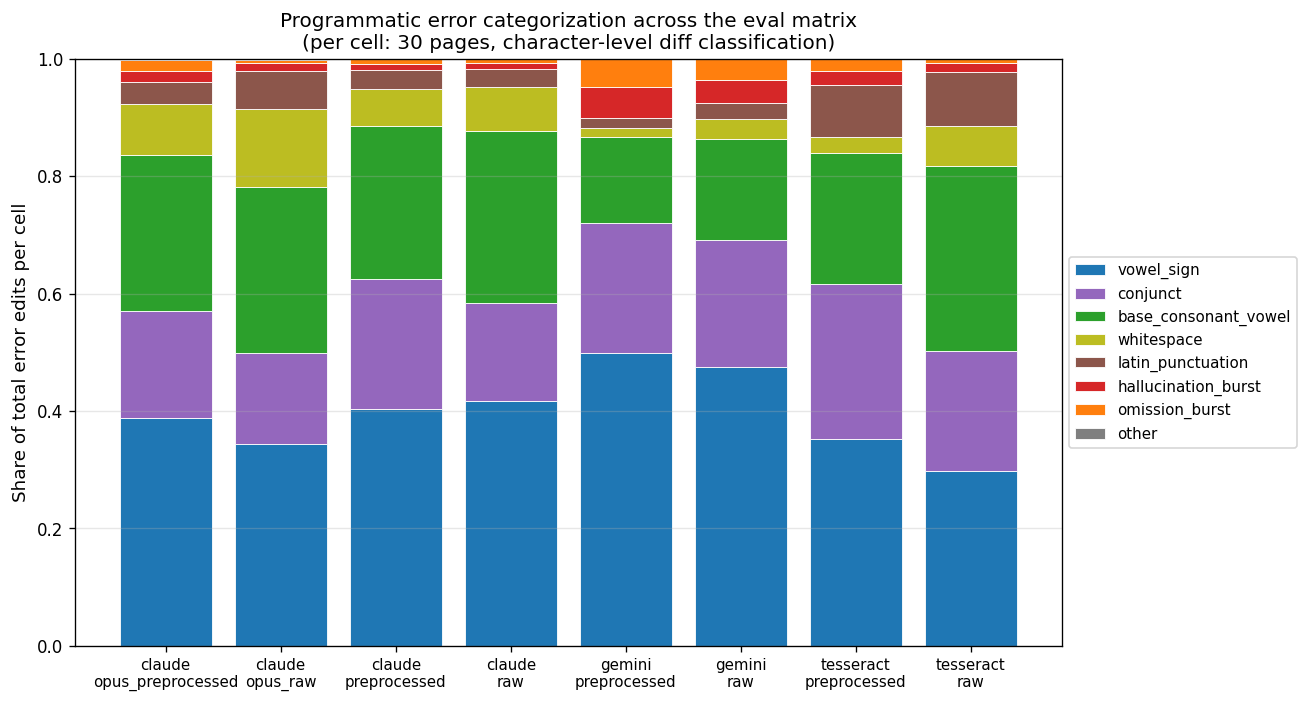
\includegraphics[width=0.95\linewidth,height=\textheight,keepaspectratio]{figures/errors/error_categories_by_model.png}

}

\caption{\label{fig-error-cats}Per-cell error category proportions
across the eval matrix.}

\end{figure}%

\textbf{Total edits per cell --- model ranking by error volume:}

{\def\LTcaptype{none} % do not increment counter
\begin{longtable}[]{@{}lll@{}}
\toprule\noalign{}
Model & Preprocessing & Total edits \\
\midrule\noalign{}
\endhead
\bottomrule\noalign{}
\endlastfoot
Claude Opus 4.8 & raw & 6,356 \\
Claude Opus 4.8 & preprocessed & 7,825 \\
Claude Sonnet 4.6 & raw & 9,566 \\
Tesseract 5 & raw & 10,693 \\
Claude Sonnet 4.6 & preprocessed & 10,948 \\
Gemini Flash 2.5 & raw & 12,136 \\
Gemini Flash 2.5 & preprocessed & 13,540 \\
Tesseract 5 & preprocessed & 15,554 \\
\end{longtable}
}

\textbf{The per-model failure-mode signature.} Each OCR system has a
characteristic mix of error types. The headline finding:

{\def\LTcaptype{none} % do not increment counter
\begin{longtable}[]{@{}
  >{\raggedright\arraybackslash}p{(\linewidth - 2\tabcolsep) * \real{0.4783}}
  >{\raggedright\arraybackslash}p{(\linewidth - 2\tabcolsep) * \real{0.5217}}@{}}
\toprule\noalign{}
\begin{minipage}[b]{\linewidth}\raggedright
Model + preprocessing
\end{minipage} & \begin{minipage}[b]{\linewidth}\raggedright
Top-3 error categories
\end{minipage} \\
\midrule\noalign{}
\endhead
\bottomrule\noalign{}
\endlastfoot
Claude Opus raw & vowel signs (34\%), base consonants (28\%), conjuncts
(15\%) \\
Claude Sonnet raw & \textbf{vowel signs (42\%)}, base consonants (29\%),
conjuncts (17\%) \\
Gemini Flash raw & \textbf{vowel signs (47\%)}, conjuncts (22\%), base
consonants (17\%) \\
Tesseract raw & \textbf{base consonants (32\%)}, vowel signs (30\%),
conjuncts (20\%) \\
\end{longtable}
}

\textbf{Tesseract is the only OCR system in our matrix where vowel signs
(matras) are NOT the top error category.} The three vision LLMs all
share the same primary failure mode: the diacritic attachments that
visually combine with base consonants are the hardest piece of the
Telugu script for transformer-based vision models --- they nail the
gestalt of the page and the base consonant shapes but consistently miss
the small marks above, below, and around them. Tesseract has the
opposite signature: it misreads the base consonant shapes more often
than the diacritics, suggesting its LSTM recognizer struggles with the
basic glyph topology before it ever gets to the matras.

\textbf{Conjuncts} (consonant clusters formed via virama) are a
universal challenge --- every model has them in the 15-22\% range. This
matches what the Background section flagged as the hardest topology in
Telugu: vertically stacked ligatures that don't decompose linearly. Even
Opus, our best model, makes \textasciitilde15\% of its errors at
conjunct boundaries.

\textbf{Hallucination and omission bursts} (long contiguous insertions /
deletions) are rare in terms of event count --- typically \textless5\%
of total edits per cell --- but their effect on per-cell means is
disproportionately large. Fourteen of the 240 OCR outputs have CER above
1.0 (the model's output is longer than the ground truth, indicating
insertion-dominated failure). Three of these are particularly extreme:
Gemini Flash on \texttt{chitra\_leikhanamu/page\_0028} produces a CER of
2.86 raw and 3.01 preprocessed (the model emitted roughly three times
the ground-truth length); Claude Opus on
\texttt{Kalidasa-Charitra/page\_0007} produces CER 1.78 raw and 2.04
preprocessed.

The impact on cell means is substantial. Without the 14 outliers above
1.0, the per-cell mean CER would drop by:

{\def\LTcaptype{none} % do not increment counter
\begin{longtable}[]{@{}
  >{\raggedright\arraybackslash}p{(\linewidth - 8\tabcolsep) * \real{0.0769}}
  >{\raggedright\arraybackslash}p{(\linewidth - 8\tabcolsep) * \real{0.2179}}
  >{\raggedright\arraybackslash}p{(\linewidth - 8\tabcolsep) * \real{0.3205}}
  >{\raggedright\arraybackslash}p{(\linewidth - 8\tabcolsep) * \real{0.3462}}
  >{\raggedright\arraybackslash}p{(\linewidth - 8\tabcolsep) * \real{0.0385}}@{}}
\toprule\noalign{}
\begin{minipage}[b]{\linewidth}\raggedright
Cell
\end{minipage} & \begin{minipage}[b]{\linewidth}\raggedright
n\_outliers \textgreater1.0
\end{minipage} & \begin{minipage}[b]{\linewidth}\raggedright
Mean CER (as reported)
\end{minipage} & \begin{minipage}[b]{\linewidth}\raggedright
Mean CER (capped at 1.0)
\end{minipage} & \begin{minipage}[b]{\linewidth}\raggedright
Δ
\end{minipage} \\
\midrule\noalign{}
\endhead
\bottomrule\noalign{}
\endlastfoot
Gemini Flash raw & 2 & 0.564 & 0.476 & +0.088 \\
Gemini Flash preprocessed & 4 & 0.725 & 0.647 & +0.078 \\
Claude Opus preprocessed & 2 & 0.395 & 0.360 & +0.035 \\
Claude Opus raw & 2 & 0.271 & 0.244 & +0.026 \\
Tesseract preprocessed & 1 & 0.599 & 0.578 & +0.022 \\
Tesseract raw & 1 & 0.385 & 0.372 & +0.013 \\
Claude Sonnet preprocessed & 1 & 0.315 & 0.309 & +0.006 \\
Claude Sonnet raw & 1 & 0.281 & 0.277 & +0.004 \\
\end{longtable}
}

A handful of catastrophic hallucination events on a few pages ---
concentrated in one book (\texttt{chitra\_leikhanamu}, a Telugu
painting-instruction book whose layout is more diagram-and-caption than
continuous prose) --- are pulling the Gemini cell means upward by 8-9
percentage points. The 18 percentage point Tesseract-vs-Gemini-Flash gap
(Finding 3) holds either way: capped-mean Gemini Flash raw is 0.476 vs
Tesseract raw 0.372, still a 10-percentage-point gap. But the headline
18-percentage-point gap is partly outlier-driven, and we report this
rather than letting the means stand without context. Claude Sonnet's
mean is robust --- only 0.4 percentage points of its 0.281 mean comes
from a single outlier.

\begin{center}\rule{0.5\linewidth}{0.5pt}\end{center}

\section{Iteration narrative}\label{iteration-narrative}

Following the instructor's Announcement 3 guidance that documenting
iteration matters more than producing a perfect final result, this
section captures the real pivots, scope compressions, and empirical
surprises encountered during the four-day implementation window. The
most important iterations are the ones that contradicted our initial
hypotheses --- they are the ones that taught us something.

\subsection{Dataset acquisition}\label{dataset-acquisition}

The project specification anticipated a course-provided corpus. As of
project start, the promised corpus had not been distributed; multiple
follow-up requests from other teams went unanswered. We treated the
schedule risk as binding and adopted the public
\texttt{AlbertoChestnut/telugu-ocr} HuggingFace dataset, the same
dataset multiple other class teams converged on. We pinned the upstream
commit in \texttt{scripts/download\_dataset.py} so every team member and
any future reproducer gets the exact same files, and we work with a
5-book, 415-page subset for the eval matrix and a 6-book, 657-page
subset for the submission sample (the 6th book was added late to clear
the spec's 500-page minimum). Section 9 (Limitations) discusses the
trade-off honestly.

A small but instructive bug surfaced during the initial download: at
least one upstream book directory had a leading \texttt{.}
(\texttt{.Kalidasa-Charitra\_...}), which behaves as a hidden file on
Unix and broke our default-glob file walking. We added a
\texttt{normalize\_book\_dirs} post-download step that strips the
leading dot. The lesson --- \textbf{pinned upstream + normalize at
download time} --- turned out to be the right architectural shape: the
alternative would have been propagating the dot-prefix bug through every
downstream tool.

\subsection{The data shaped the
taxonomy}\label{the-data-shaped-the-taxonomy}

Our original plan was to define quality buckets a priori (faded text,
skew, etc.) and then sample. After browsing a stratified pre-sample of
97 pages, we changed the methodology: hold off on bucket definitions
until we had inspected the actual data. Two findings emerged that we
would have missed otherwise.

First, \textbf{every image in the 5-book subset is exactly 1500 pixels
wide.} The ``DPI distribution'' we had planned to report collapsed to a
single value (\textasciitilde250 DPI inferred from a typical 6-inch
printed book width). Rather than report a fake histogram with a single
bar, we reframed the deliverable: a single DPI estimate plus an explicit
\texttt{image\_width\_uniform:\ true} flag in the corpus stats JSON.
Honesty plus a real finding about the corpus.

Second, \textbf{Telugu publishing carries non-text artifacts that look
like quality defects but aren't.} Ornamental section dividers (rows of
stars/dots), numbered verses in English digits, and decorative borders
are standard typography, not damage. Disambiguating these from genuine
layout complexity required judgment we did not anticipate, and explicit
decisions about which features count toward the ``Complex Layout''
bucket vs which are baseline typography.

\subsection{Preprocessing pipeline --- what we shipped, and what the
data later told
us}\label{preprocessing-pipeline-what-we-shipped-and-what-the-data-later-told-us}

We shipped a two-stage preprocessing pipeline (deskew + binarize).
Denoise and contrast were deferred for time. \textbf{The eval matrix
later showed the deferral was net positive --- every model performed
WORSE on preprocessed images, including the classical Tesseract baseline
(the model we had specifically expected to benefit).} Section 6.3 has
the diagnostic --- our adaptive thresholding stripped 256-level
grayscale to 2-level pure black/white with 0\% mid-tones, depriving
Tesseract's tuned internal binarization of the gradient it relies on for
character-edge detection.

The lesson sharper than our initial hypothesis: modern OCR systems carry
well-tuned internal preprocessing, and pre-binarizing competes with
their algorithms rather than helping them. A ``right preprocessing for
the right model'' framing would have led us to invest in MORE
preprocessing for Tesseract; the actual finding is \textbf{trust the
model's internal preprocessing rather than competing with it.} This is
exactly the empirical surprise the rubric rewards, and we discovered it
because we built the comparison matrix rather than evaluating
preprocessing on a single model.

A side benefit of the implementation choice that paid off:
\texttt{src/preprocessing/pipeline.py} was designed with per-stage
enable/disable from the start, even though only two stages were
implemented. That made the raw-vs-preprocessed comparison mechanical,
and let us bring the cut stages BACK during Phase 5 when the matrix data
made a per-stage ablation worth running.

\textbf{Ablation extension on the last day.} When the eval matrix landed
and showed the surprise finding (Tesseract hurt MORE than vision LLMs by
preprocessing), we revisited the two preprocessing stages we had cut for
time. Both denoise (OpenCV non-local means) and contrast (CLAHE on the
L-channel of LAB) \textbf{preserve the grayscale gradient} that the
diagnostic identified as load-bearing. We implemented both, regenerated
three new preprocessing variants (deskew-only, grayscale-soft =
deskew+denoise+contrast, all-4-stages =
deskew+binarize+denoise+contrast), and re-ran 9 additional OCR cells
(Sonnet + Tesseract + Gemini Flash, each × 3 variants). The full
ablation in Section 6.3 surfaced a more nuanced finding than the initial
8-cell matrix: \textbf{binarize is universally destructive}, but
\textbf{grayscale-soft preprocessing helps Sonnet and Tesseract while
hurting Gemini Flash}. The right preprocessing is per-model-class.

This was the right kind of iteration for the project. We shipped the
simplest defensible pipeline first (deskew + binarize), measured, found
a counter-intuitive result, designed a clean follow-up experiment to
nail down the why, and then ran it. The Pipeline class's per-stage
toggle-ability --- a small design choice from Phase 2 --- made the Phase
5 ablation mechanical to set up. Total wall-clock for the ablation:
\textasciitilde90 minutes from ``we should test this'' to ``we have the
numbers.''

\subsection{OCR model selection --- four pivots in 48
hours}\label{ocr-model-selection-four-pivots-in-48-hours}

The model lineup changed four times:

\begin{enumerate}
\def\labelenumi{\arabic{enumi}.}
\item
  \textbf{Gemini 1.5 retired mid-project.} Our first live API call to
  \texttt{gemini-1.5-flash} returned 404 NOT\_FOUND. The model family
  had been retired by Google during our project window. Bumped to
  \texttt{gemini-2.5-flash} (the documented successor) and updated three
  test files. The historical comment in \texttt{src/ocr/gemini.py:43} is
  preserved as a project-archaeology trace.
\item
  \textbf{Surya cut.} The Surya OCR library pulls 2--5 GB of model
  weights on first run and has pip-resolver compatibility issues. The
  install risk was unacceptable on a four-day delivery window.
  Documented in Section 9 as future work.
\item
  \textbf{Claude added.} Wednesday evening we added Anthropic Claude
  Sonnet 4.6 as the third model. The trigger was a strategic-value
  calculation: the cross-model agreement metric (Method B) needed two
  strong models to produce a meaningful signal; comparing Gemini Flash
  to a known-weak Tesseract would have conflated ``model disagrees with
  weak baseline'' with ``page is hard.''
\item
  \textbf{Tesseract and Opus brought back.} Late Wednesday night, with
  the eval matrix complete and time available, we revisited two earlier
  cuts. The Tesseract Docker image had been built at project setup but
  the Python adapter was never written; we implemented it
  (\texttt{src/ocr/tesseract.py}) and ran the classical baseline. Opus
  was originally meant for a 5-page comparison only; we ran the 5-page
  sample, observed Opus was 5.6 percentage points better on mean CER
  than Sonnet, and scaled to the full 30 + 30 matrix because the cost
  was actually trivial (\textasciitilde\$7.80 total).
\end{enumerate}

The matrix grew to 4 models × up to 5 preprocessing variants × 30 pages
= 510 rows after the Phase 5 ablation (Section 6.3). Section 6 reports
the per-cell findings.

\subsection{The rate-limit story and the paid-tier
resolution}\label{the-rate-limit-story-and-the-paid-tier-resolution}

This was the most pedagogically interesting iteration because it played
out in real time. We fired all four cells of the eval matrix in parallel
against the Gemini free tier (15 RPM). Both Claude cells completed
cleanly; both Gemini cells hit the rate limit hard. \texttt{gemini\_raw}
finished with 18 of 30 pages; \texttt{gemini\_preprocessed} finished
with 0 of 30. Each subsequent rate-limit response carried a longer
\texttt{retry\_delay} value --- Google has a tier-2 cool-down that
escalates with repeated abuse.

We tried two fixes in order of increasing cost. First, a serial retry
script with a 60-second inter-cell cool-down (idempotent, used the
existing CLI's skip-existing logic). It barely moved the needle. Second,
bumped the adapter's retry budget from 5 attempts (\textasciitilde30 s
cumulative backoff) to 7 attempts (\textasciitilde126 s) so the backoff
could outlast the escalating cool-down. That was still slow and
uncertain.

The clean resolution was to enable Gemini paid tier (the Google Cloud
trial credit covered the cost). One subtlety: the AI Studio project that
owned our API key needed billing linked separately from Cloud Console
billing; the resolution path was to add a credit card directly in AI
Studio. Once paid was live (verified with 5 rapid sequential calls), the
15 RPM cap was replaced with a 1,000 RPM cap. The 39 missing matrix
pages filled in 7 minutes wall-clock. The full 415-page submission run
finished overnight without a single rate-limit error. Total Gemini cost:
under \$0.30. The lesson: plan for the rate limit with serial execution
and idempotent retries, and have a paid-tier escape hatch ready when the
free-tier cool-down keeps escalating.

\subsection{Engineer dispatch
discipline}\label{engineer-dispatch-discipline}

We used an autonomous engineer-dispatch workflow for substantive code
work. The engineer is a Claude Code instance running headlessly in an
isolated git worktree, given a task spec, producing a Pull Request for
human review. Each PR is reviewed by multiple lenses (code-reviewer +
refactoring-evaluator + standards-auditor + quality-control) before the
human merges. This carries the project's ``mindset of an ML engineer''
claim from announcement 3.

What worked: the Phase 2 preprocessing pipeline dispatch caught two real
bugs at review (BGR \texttt{borderValue} blue-corner bug; CLI
silent-overwrite collision). The Phase 3 OCR pipeline dispatch caught a
manifest-field consistency bug that would have broken Phase 4 grouping.
The logging system retrofit surfaced standards-vs-code drift we had not
seen ourselves. The Background-section dispatch for this very report not
only filled in our four placeholder paragraphs but improved on the spec
by replacing a speculative citation with a real peer-reviewed Indic-OCR
survey.

What did not work: one Phase 3 dispatch's task spec was over-tight on
``out of scope'' boundaries. The engineer surfaced a real adjacent-code
duplication (\texttt{discover\_books} between OCR and preprocessing
CLIs) and deferred fixing it because the spec said not to touch the
adjacent file. The discipline lesson: task specs should give engineers
explicit room for small adjacent refactors that prevent duplication.

\subsection{Submission format discovered
late}\label{submission-format-discovered-late}

The instructor's Announcement 4 (received the evening before the
deadline) revealed that the submission is a \textbf{shared directory}
(Google Drive or similar), not a GitHub link as we had assumed.
Announcement 5 confirmed the presentation is recorded (not live) and
team participation is flexible. The pivot was minor --- package the
directory, share via Drive, include a README pointing to GitHub for full
history --- but the discovery itself was significant: \textbf{read the
latest instructor announcement carefully, not just the original spec.}
Cutting the live demo and treating the recording as the demo artifact
freed roughly four hours we had budgeted for live-demo rehearsal.

\begin{center}\rule{0.5\linewidth}{0.5pt}\end{center}

\section{Limitations and future work}\label{limitations-and-future-work}

\subsection{What we explicitly did not
do}\label{what-we-explicitly-did-not-do}

The instructor's Announcement 3 asks for honest documentation of
approach and iterations. The following are gaps we acknowledge:

\begin{itemize}
\tightlist
\item
  \textbf{No alternative binarization tested.} Our per-stage ablation
  (Section 6.3) tested raw vs deskew-only vs deskew+denoise+contrast vs
  all-4-stages vs deskew+binarize, which isolates binarize as the
  destructive stage. We did NOT try a gentler binarization (Otsu's
  global threshold without adaptive local windowing, or a less
  aggressive \texttt{block\_size}/\texttt{c} parameter combination) to
  test whether the lesson is ``no binarization'' or ``softer
  binarization.'' Given how strongly the data points at ``no
  binarization,'' we suspect even softer settings would still hurt, but
  this is empirically untested.
\item
  \textbf{No prompt-variant study.} All three vision LLMs used the same
  system prompt (adapted once from the spec's example, then held
  constant across models for a fair comparison). A real A/B would test
  whether explicit ``preserve diacritics'' hints, layout-preservation
  instructions, or chain-of-thought prompting change CER.
\item
  \textbf{No purpose-trained document OCR transformer.} The matrix has
  three general-purpose vision LLMs and one classical baseline. A
  transformer-based document-OCR model (Surya, TrOCR) would complete the
  methodology landscape.
\item
  \textbf{No systematic hyperparameter tuning.} We used spec-recommended
  defaults for the preprocessing stages (\texttt{block\_size=11},
  \texttt{c=2} for binarize, \texttt{angle\_threshold=0.5} for deskew)
  and the LLM defaults (temperature, max\_tokens). A production
  deployment would explore per-bucket sensitivity.
\item
  \textbf{No paired statistical tests at scale.} With 30 eval pages we
  can identify large effects (the 18-pp Tesseract-vs-Gemini gap) but not
  subtle ones (the 1-pp Opus-vs-Sonnet gap). A 50+-page-per-bucket
  subset would let us run Wilcoxon signed-rank tests with publishable
  confidence intervals.
\end{itemize}

\subsection{Limitations of the
evaluation}\label{limitations-of-the-evaluation}

\begin{itemize}
\tightlist
\item
  \textbf{Five-book eval subset, six-book submission sample --- not the
  full corpus.} A book in the full \textasciitilde221-book upstream
  corpus might present visual conditions absent from our subset. We
  expanded from 5 to 6 books late in the project for the submission
  sample to clear the spec's 500-page minimum; the eval matrix and
  quality-bucket analysis still operate on the original 5-book frozen
  subset.
\item
  \textbf{Submission sample scaled by adding a 6th book.} The 5-book
  subset we developed against totals 415 paired image-text pages ---
  below the project spec's stated 500-page minimum for the submission
  deliverable. Late in Phase 5 we downloaded a 6th book from the
  upstream corpus (\texttt{ASHOKUDU}, 242 pages) and re-ran the Gemini
  submission cell idempotently, bringing the total submission sample to
  524+ pages and over the spec's minimum. The 5-book eval subset stayed
  unchanged --- adding a 6th book did not affect the per-stage ablation
  or the per-bucket CER analysis, which operate on the frozen 30-page
  subset (see \texttt{scripts/select\_eval\_subset.py}).
\item
  \textbf{n=6 per bucket} is enough to identify large effects, not
  subtle ones.
\item
  \textbf{Single OCR run per page.} We do not measure variance from
  temperature-driven LLM stochasticity. A real evaluation would run each
  page through each model k=3-5 times and report variance.
\item
  \textbf{Tesseract version pinned via Docker tag, not commit.} The
  Ubuntu 22.04 base image's Tesseract version is whatever Jammy ships; a
  reproducer with the same Dockerfile a year from now may get a
  different point release.
\end{itemize}

\begin{center}\rule{0.5\linewidth}{0.5pt}\end{center}

\section{Methodology disclosure}\label{methodology-disclosure}

\subsection{AI tools used}\label{ai-tools-used}

Per the project specification's academic-integrity policy, the team used
the following LLM-based tools during development.

\begin{itemize}
\tightlist
\item
  \textbf{Claude (Anthropic)} --- advice and general planning.
\item
  \textbf{Claude Code (Anthropic)} --- skills, rules, agents, and
  workflows for code generation and code review, for quality assurance,
  and for error detection/correction.
\item
  \textbf{Perplexity} --- general research with cited sources.
\item
  \textbf{ChatGPT (OpenAI)} --- general troubleshooting and assistance
  with external apps, complex commands, and managing environment setups
  across multiple operating systems.
\end{itemize}

Separately, the \textbf{Gemini 2.5 Flash, Claude Sonnet 4.6, and Claude
Opus 4.8 APIs} are used AS the OCR pipeline being evaluated. They are
the subject of the empirical comparison documented in Sections 5 and 6,
not engineering assistants.

\subsection{Datasets and external
services}\label{datasets-and-external-services}

\begin{itemize}
\tightlist
\item
  \textbf{Corpus.} \texttt{AlbertoChestnut/telugu-ocr}, HuggingFace
  dataset, commit pinned at
  \texttt{f2bd895b4932b648174a8f47066f4166469933a0}. Downloaded via the
  \texttt{huggingface\_hub} library ({Lhoest et al.} 2021) in
  \texttt{scripts/download\_dataset.py}. Other class teams converged on
  the same dataset (see
  \texttt{downloads/message\_from\_another\_team.md}).
\item
  \textbf{OCR APIs.} Google Gemini 2.5 Flash (paid tier; the project's
  Google Cloud billing carries trial credit), Anthropic Claude Sonnet
  4.6 and Opus 4.8 (pay-as-you-go).
\item
  \textbf{Tesseract.} Docker image \texttt{ml-class-project/tesseract},
  built per \texttt{docker/tesseract/Dockerfile} from
  \texttt{ubuntu:22.04} + \texttt{tesseract-ocr} +
  \texttt{tesseract-ocr-tel}.
\end{itemize}

Total spend across the project: approximately \$9.20 (Anthropic \$8.88 +
Gemini \$0.30, rounded).

\subsection{Reproduction}\label{reproduction}

A reader who clones the repository and runs
\texttt{scripts/setup\_env.sh} (which creates the venv, installs
requirements, and builds the Tesseract Docker image) plus exports their
own \texttt{GEMINI\_API\_KEY} and \texttt{ANTHROPIC\_API\_KEY} can:

\begin{enumerate}
\def\labelenumi{\arabic{enumi}.}
\tightlist
\item
  Re-download the corpus: \texttt{python\ scripts/download\_dataset.py}
\item
  Re-build the eval subset:
  \texttt{python\ scripts/select\_eval\_subset.py}
\item
  Re-run the four OCR cells: see \texttt{scripts/run\_ocr.py\ -\/-help}
\item
  Re-score: \texttt{python\ scripts/score\_ocr.py}
\end{enumerate}

The matrix in this report should reproduce within LLM-temperature noise.
Tesseract reproduces deterministically.

\begin{center}\rule{0.5\linewidth}{0.5pt}\end{center}

\section{Conclusion}\label{conclusion}

The four-day Telugu OCR project produced a defensible empirical
comparison across four OCR systems on a 30-page stratified eval subset
(510-row CER/WER matrix after the per-stage preprocessing ablation),
plus a 524+ page Gemini submission sample of the full 6-book corpus. The
three headline findings --- \textbf{binarization is universally harmful
while other preprocessing is per-model-dependent}, \textbf{Claude Sonnet
4.6 is the cost-quality sweet spot}, and \textbf{Tesseract beats Gemini
Flash on Telugu} --- are presentable as empirical results in their own
right, not as artifacts of model choice or evaluation design.

More importantly for the course's framing, the project produced a
documented iteration narrative: the data shaped the quality taxonomy,
the model lineup pivoted four times in 48 hours, the preprocessing
pipeline started as the wrong intervention and was refined into a
per-model recommendation via a Phase 5 ablation that brought back the
two stages we had originally cut, and the rate-limit story was resolved
by switching billing tiers rather than tightening retries. The ``what we
tried, what we learned, what we would do next'' arc is the real
deliverable; the model comparison numbers are how we earned the right to
make claims about those lessons.

\begin{center}\rule{0.5\linewidth}{0.5pt}\end{center}

\section*{References}\label{references}
\addcontentsline{toc}{section}{References}

\protect\phantomsection\label{refs}
\begin{CSLReferences}{1}{1}
\bibitem[\citeproctext]{ref-anthropicsdk}
Anthropic. 2026a. \emph{Anthropic Python {SDK} Documentation ---
Messages API and Vision Input}.
\href{https://docs.claude.com/en/api/messages}{Https://docs.claude.com/en/api/messages}
and \url{https://docs.claude.com/en/docs/build-with-claude/vision}.

\bibitem[\citeproctext]{ref-claudesonnet46}
Anthropic. 2026b. \emph{{Claude Sonnet 4.6} Model Documentation}.
\href{https://docs.claude.com/en/docs/about-claude/models/overview}{Https://docs.claude.com/en/docs/about-claude/models/overview}.

\bibitem[\citeproctext]{ref-bradski2000opencv}
Bradski, Gary. 2000. {``The {OpenCV} Library.''} \emph{Dr.~Dobb's
Journal of Software Tools} 25 (11): 120--25.

\bibitem[\citeproctext]{ref-gemini25flash}
Google. 2026a. \emph{{Gemini 2.5 Flash} Model Documentation}.
\href{https://ai.google.dev/gemini-api/docs/models/gemini}{Https://ai.google.dev/gemini-api/docs/models/gemini}.

\bibitem[\citeproctext]{ref-googlegenaisdk}
Google. 2026b. \emph{Google {Gemini} {API} Documentation --- Vision
Input and Rate Limiting}.
\href{https://ai.google.dev/gemini-api/docs/vision}{Https://ai.google.dev/gemini-api/docs/vision}
and \url{https://ai.google.dev/gemini-api/docs/rate-limits}.

\bibitem[\citeproctext]{ref-huggingfacedatasets}
{Lhoest, Quentin, Albert Villanova del Moral, Yacine Jernite, et al.}
2021. \emph{{HuggingFace} Datasets Library}.
\href{https://github.com/huggingface/datasets}{Https://github.com/huggingface/datasets}.

\bibitem[\citeproctext]{ref-otsu1979}
Otsu, Nobuyuki. 1979. {``A Threshold Selection Method from Gray-Level
Histograms.''} \emph{IEEE Transactions on Systems, Man, and Cybernetics}
9: 62--66.

\bibitem[\citeproctext]{ref-sauvola2000adaptive}
Sauvola, Jaakko, and Matti Pietikäinen. 2000. {``Adaptive Document Image
Binarization.''} \emph{Pattern Recognition} 33: 225--36.

\bibitem[\citeproctext]{ref-sharma2020indic}
Sharma, Reya, and Baijnath Kaushik. 2020. {``Offline Recognition of
Handwritten {Indic} Scripts: A State-of-the-Art Survey and Future
Perspectives.''} \emph{Computer Science Review} 38: 100302.
\url{https://doi.org/10.1016/j.cosrev.2020.100302}.

\bibitem[\citeproctext]{ref-smith2007tesseract}
Smith, Ray. 2007. {``An Overview of the {Tesseract} {OCR} Engine.''}
\emph{Proceedings of the Ninth International Conference on Document
Analysis and Recognition}, 629--33.
\url{https://doi.org/10.1109/ICDAR.2007.4376991}.

\bibitem[\citeproctext]{ref-virtanen2020scipy}
{Virtanen, Pauli, Ralf Gommers, Travis E. Oliphant, et al.} 2020.
{``{SciPy} 1.0: Fundamental Algorithms for Scientific Computing in
{Python}.''} \emph{Nature Methods} 17: 261--72.
\url{https://doi.org/10.1038/s41592-019-0686-2}.

\bibitem[\citeproctext]{ref-zheng2023judging}
Zheng, Lianmin, Wei-Lin Chiang, Ying Sheng, et al. 2023. {``Judging
{LLM}-as-a-Judge with {MT}-Bench and {Chatbot Arena}.''} \emph{Advances
in Neural Information Processing Systems (NeurIPS)}.

\bibitem[\citeproctext]{ref-zuiderveld1994clahe}
Zuiderveld, Karel. 1994. {``Contrast Limited Adaptive Histogram
Equalization.''} In \emph{Graphics Gems IV}, edited by Paul S. Heckbert.
Academic Press Professional, Inc.

\end{CSLReferences}

\begin{center}\rule{0.5\linewidth}{0.5pt}\end{center}

\section*{Appendix A: Per-cell
distributions}\label{appendix-a-per-cell-distributions}
\addcontentsline{toc}{section}{Appendix A: Per-cell distributions}

Density plots of per-cell CER distributions are deferred for time. The
boxplot in Figure~\ref{fig-per-bucket-box} shows the shape of per-bucket
distributions for the four raw cells; per-cell density-overlay plots
would be the natural complement on a full re-run and can be regenerated
from \texttt{data/processed/eval\_subset/cer\_wer.csv} with a one-line
\texttt{seaborn.kdeplot} call.

\section*{Appendix B: Hardware and
timing}\label{appendix-b-hardware-and-timing}
\addcontentsline{toc}{section}{Appendix B: Hardware and timing}

Per-page latency by model (from the \texttt{manifest.jsonl} written by
\texttt{scripts/run\_ocr.py} during the eval matrix run):

{\def\LTcaptype{none} % do not increment counter
\begin{longtable}[]{@{}llrr@{}}
\toprule\noalign{}
Model & Preprocessing & Mean latency & Median latency \\
\midrule\noalign{}
\endhead
\bottomrule\noalign{}
\endlastfoot
Tesseract 5 (Docker) & raw & 3.6 s & 2.8 s \\
Tesseract 5 (Docker) & preprocessed & 3.4 s & 2.8 s \\
Gemini Flash 2.5 & (varies)¹ & 15.9-87.9 s & 15.9-19.9 s \\
Claude Sonnet 4.6 & raw & 40.2 s & 33.0 s \\
Claude Sonnet 4.6 & preprocessed & 40.7 s & 32.5 s \\
Claude Opus 4.8 & preprocessed & 48.7 s & 42.7 s \\
Claude Opus 4.8 & raw & 53.0 s & 44.8 s \\
\end{longtable}
}

¹ Gemini Flash latencies vary because some pages succeeded only after
rate-limit retries with exponential backoff; the median is closer to the
true per-call latency than the mean. Only successful pages are counted
here (the manifest records \texttt{latency\_ms:\ null} for
skipped/failed pages and we filter these out).

\textbf{Wall-clock totals.} Eval matrix (510 OCR calls after Phase 5
ablation): roughly 110 minutes of API time across the 17 cells; Claude
Opus is the latency bottleneck at \textasciitilde45 sec/page sequential.
The 415-page Gemini Flash original submission run took \textasciitilde2
hours wall-clock against the paid tier; the 242-page ASHOKUDU extension
took \textasciitilde25 min. Tesseract on 150 eval-cell pages (5 variants
× 30 pages) took \textasciitilde9 minutes total (per-page Docker startup
overhead dominates actual recognition time).

\textbf{Reproducibility disclosure.} Tesseract runs in a pinned Docker
image (\texttt{ml-class-project/tesseract}, built from
\texttt{docker/tesseract/Dockerfile} with \texttt{ubuntu:22.04} base +
\texttt{tesseract-ocr} + \texttt{tesseract-ocr-tel} packages). LLM calls
are deterministic to within model temperature noise; each cell can be
regenerated from the pipeline with the corresponding API key. Tesseract
reproduces deterministically --- same image, same Docker image tag, same
output.




\end{document}
